\section{Auswertung}
\label{sec:Auswertung}

Die Graphen werden sowohl mit Matplotlib \cite{matplotlib} als auch NumPy \cite{numpy} erstellt. Die Fehlerrechnung wird mithilfe von Uncertainties \cite{uncertainties} durchgeführt. Die Peaks der Spektren wurden mithilfe von Scipy \cite{scipy} bestimmt. Die Fehler auf die Frequenzen ergeben sich, soweit nicht anders angegeben, aus der Schrittweite.

\subsection{Modellierung: Teilchen im Potentialtopf}

In Abbildung \ref{fig:Uebersicht} ist das Übersichtsspektrum für eine $\SI{600}{\milli\meter}$-Röhre und in Abbildung \ref{fig:150} das einer $\SI{150}{\milli\meter}$-Röhre zu sehen.
Eine zweite Messung des Spektrums letzterer, liefert abgesehen von geringen Abweichungen in der Amplitude dasselbe Spektrum.
Beispielhaft sind die Parameter des 1. Peaks der beiden Messungen in Tabelle \ref{tab:param} zu sehen.

\begin{figure}
\centering
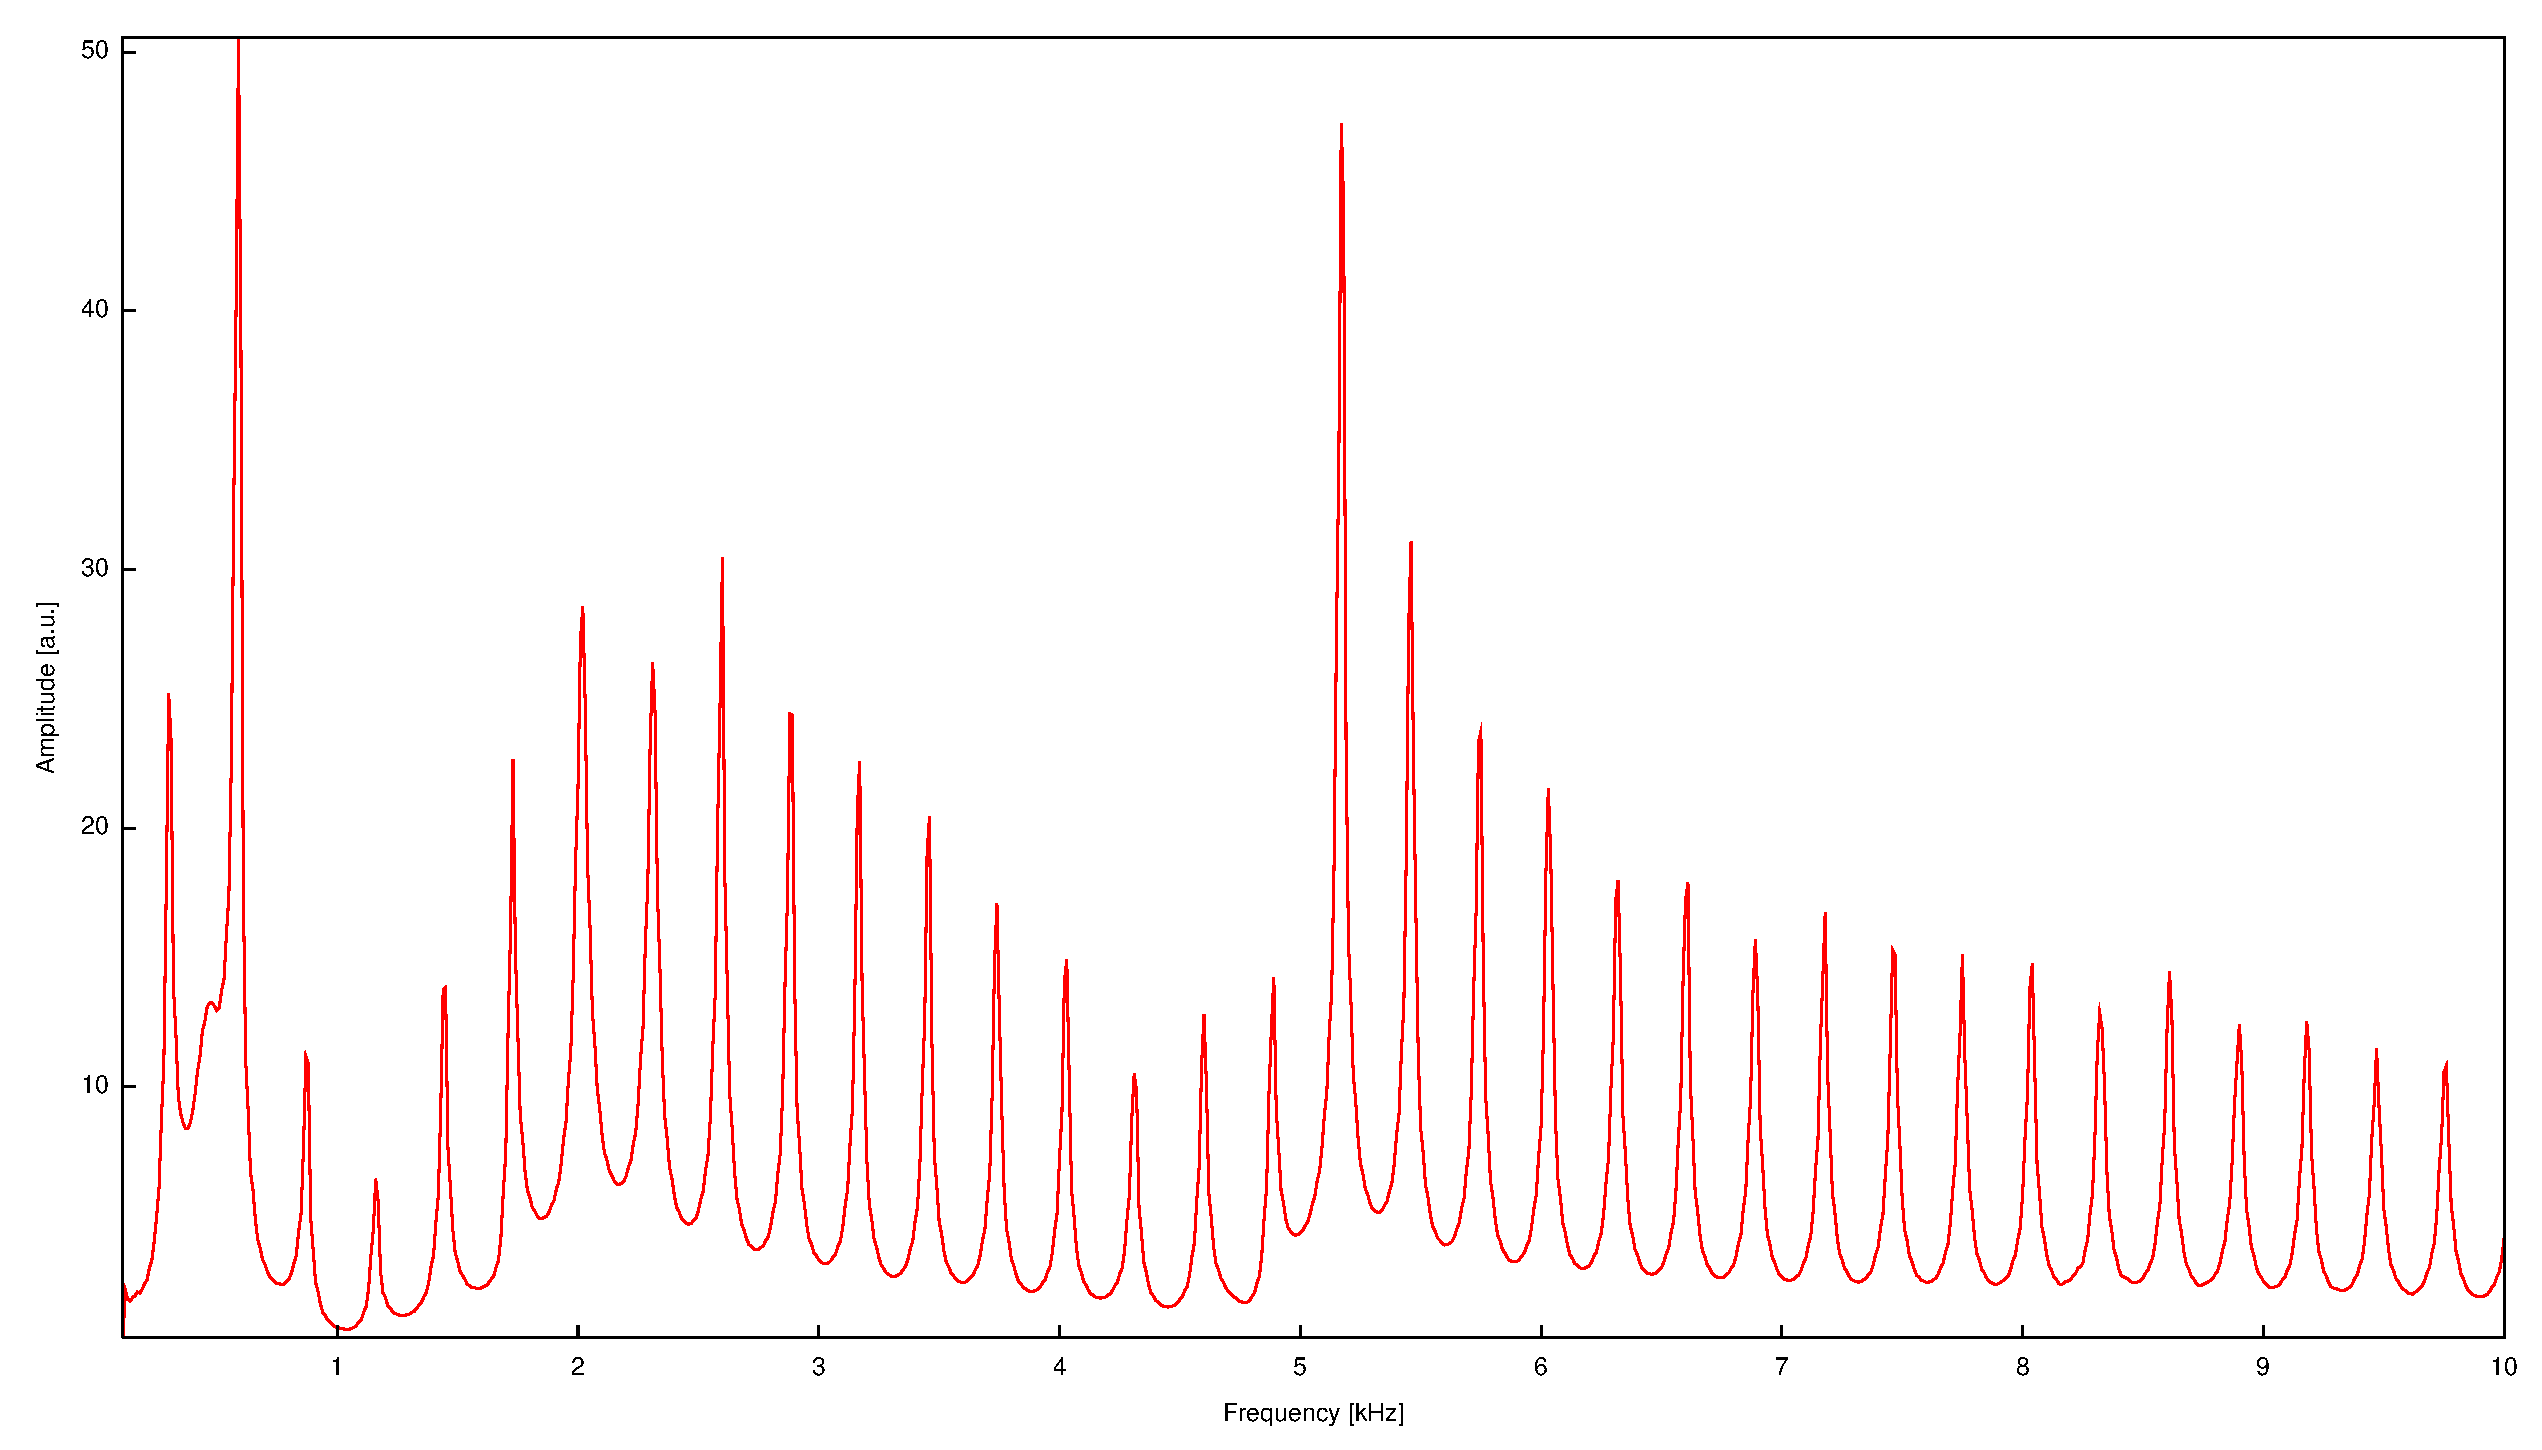
\includegraphics[width=\linewidth-70pt,height=\textheight-70pt,keepaspectratio]{FP-V23data/1.1_600mm.eps}
\caption{Spektrum einer $\SI{600}{\milli\meter}$-Röhre.}
\label{fig:Uebersicht}
\end{figure}

\begin{figure}
\centering
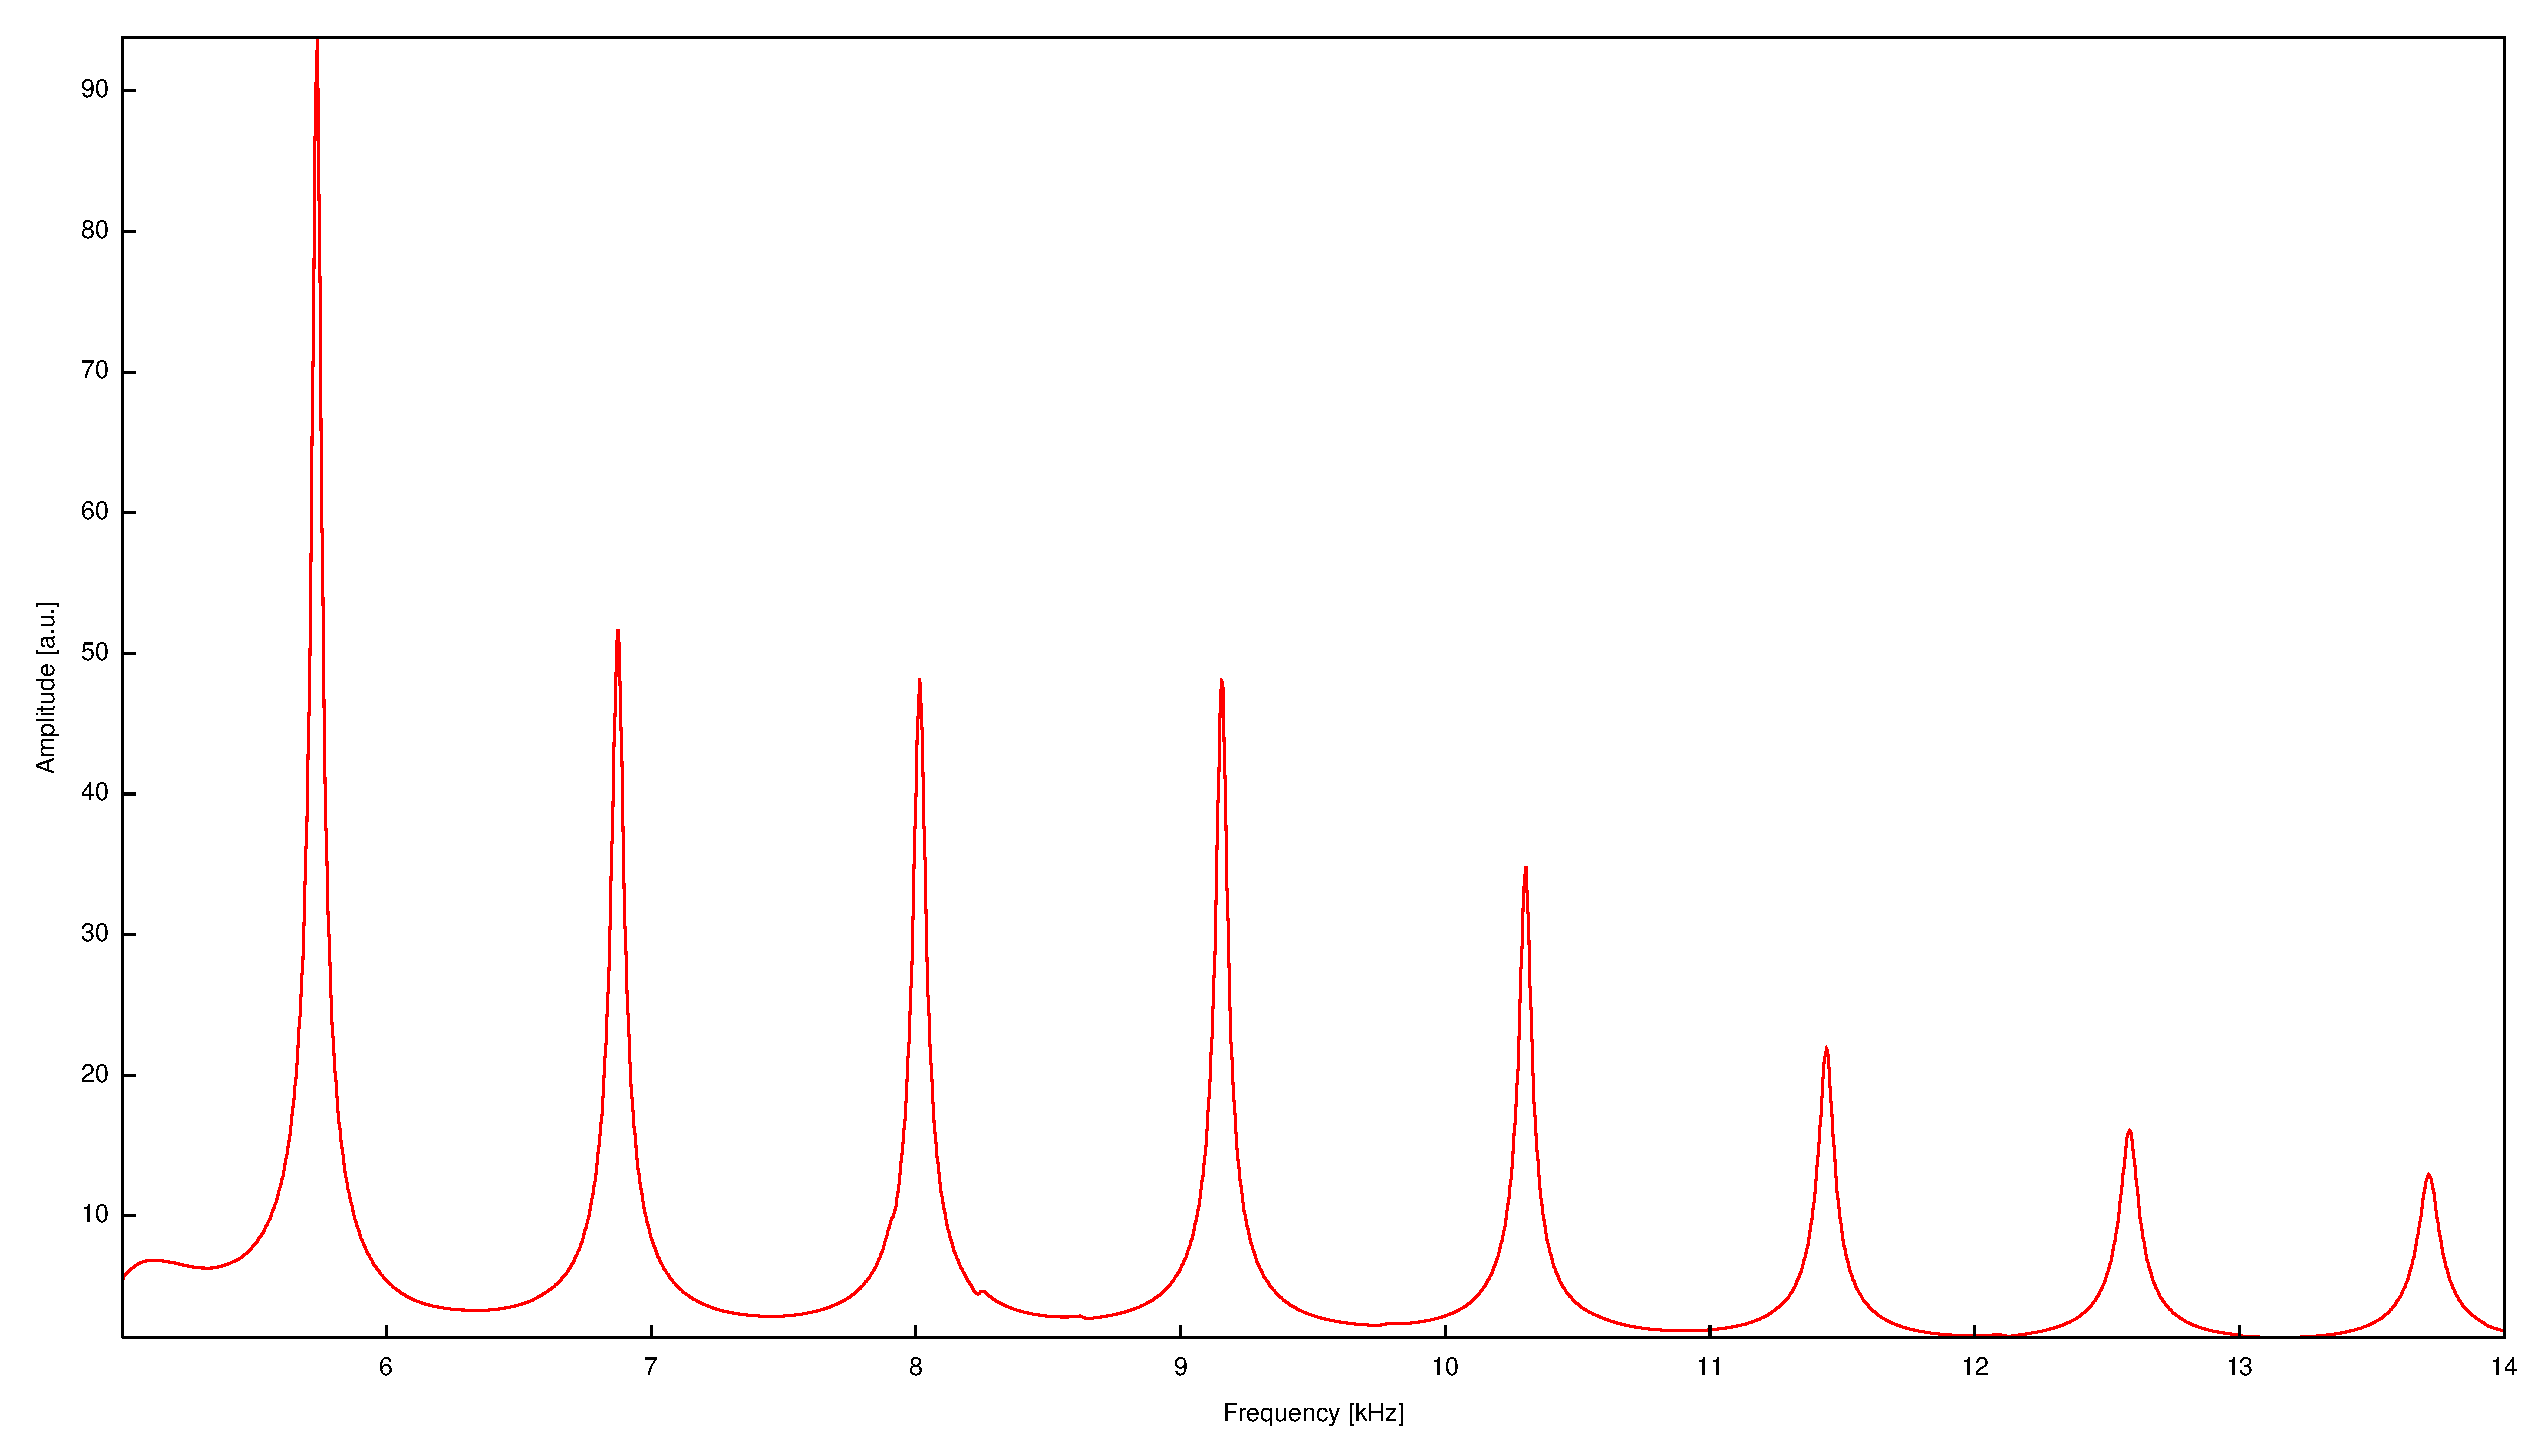
\includegraphics[width=\linewidth-70pt,height=\textheight-70pt,keepaspectratio]{FP-V23data/1.2(4.1)_150mm.eps}
\caption{Spektrum einer $\SI{150}{\milli\meter}$-Röhre.}
\label{fig:150}
\end{figure}

\begin{table}
\caption{Parameter des 1. Peaks von zwei spektralen Analysen einer $\SI{600}{\milli\meter}$ langen Röhre.}
\centering
\label{tab:params}
	\sisetup{table-format=1.2}
	\begin{tabular}{S[table-format=1.0]S[table-format=4.3]S[table-format=2.4]}
		\toprule
		{Messung} & {$f_\text{1}/(\si{\hertz})$} & {$A_\text{1}/(\si{a\text{.}u\text{.}})$} \\
		\midrule
		 1 & 5747.706 & 92.8953 \\
		 2 & 5747.706 & 92.0576 \\
		\bottomrule
	\end{tabular}

\label{tab:param}
\end{table}

\subsection{Modellierung: Das Wasserstoffatom}

In den Abbildungen \ref{fig:Overview1} und \ref{fig:Overview2} sind das Spektrum des sphärischen Resonators bei $\alpha=\SI{0}{\degree}$ und $\alpha=\SI{180}{\degree}$
zu sehen.
Die Resonanzfrequenzen $f_.n$ verändern sich nicht, jedoch fällt auf, dass bei $\alpha=\SI{0}{\degree}$ die Amplitude des 2. Peaks das Spektrum dominiert, während bei $\alpha=\SI{180}{\degree}$ alle Peaks in etwa dieselbe Höhe haben. Außerdem zeigt sich, dass in diesem Spektrum alle Peaks eine größere Amplitude aufweisen, als bei $\alpha=\SI{0}{\degree}$.\\
In den Abbildungen \ref{fig:5k_Peak1} und \ref{fig:5k_Peak2} ist für $\alpha=\SI{0}{\degree}$ und für $\alpha=\SI{40}{\degree}$, der Peak bei $f\approx\SI{5000}{\hertz}$ näher aufgelöst.
Es zeigt sich das der Hauptpeak mit zunehmendem $\alpha$ leicht zunimmt. Bei $\alpha=\SI{40}{\degree}$ bildet sich ein stark zunehmender Nebenpeak aus, der bei $\alpha=\SI{0}{\degree}$ von einer Einbuchtung überlagert wird.\\
In Abbildung \ref{fig:polar} sind die Polarplots der Peaks im Bereich von $\SI{2000}{\hertz}$ bis $\SI{7000}{\hertz}$ zu sehen.
Der Vergleich mit Bildern aus der Literatur \cite{V23}, liefert den Zusammenhang zwischen den ersten vier Peaks und den Kugelflächenfunktionen:
\begin{align*}
.{Peak 1}&\mathop{\widehat{=}} Y^0_1\\
.{Peak 2}&\mathop{\widehat{=}} Y^0_2\\
.{Peak 3}&\mathop{\widehat{=}} Y^0_3\\
.{Peak 4}&\mathop{\widehat{=}} Y^0_4\\
\end{align*}
Der 5. Polarplot lässt sich keinem Zustand mit $m=0$ zuordnen und ähnelt am ehesten der Kugelflächenfunktion $Y^.1_.2$.

\begin{figure}
\centering
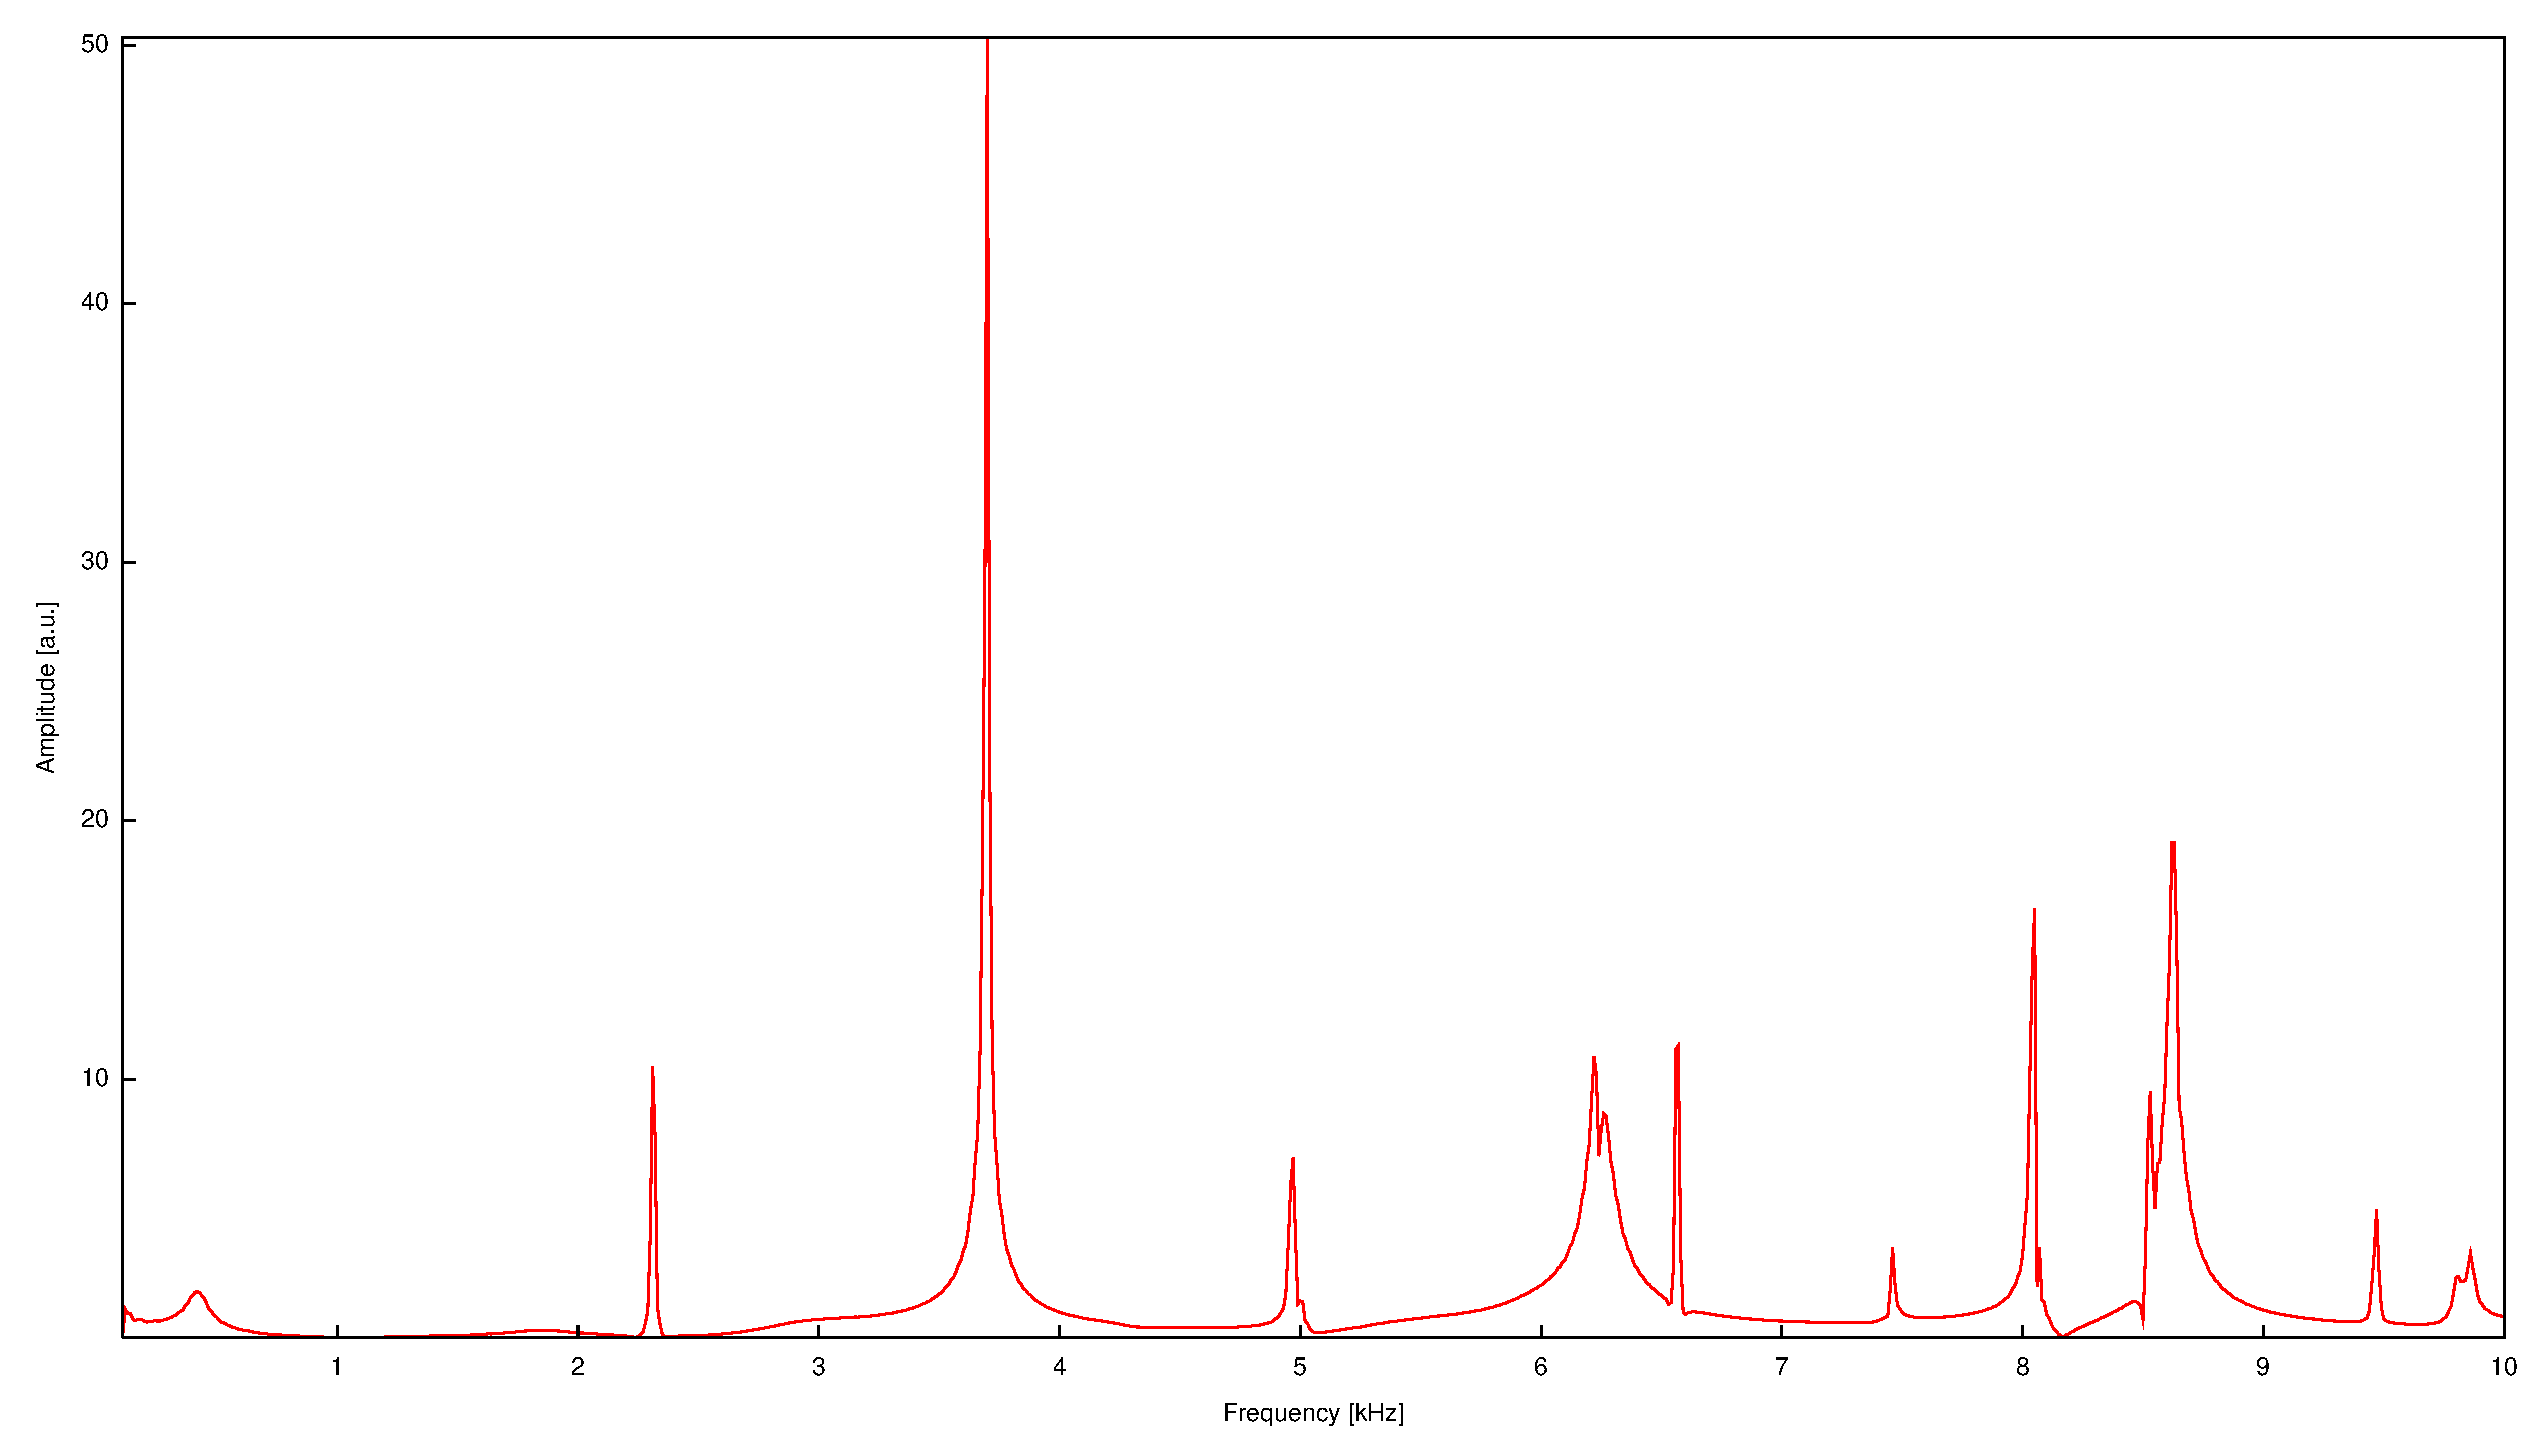
\includegraphics[width=\linewidth-60pt,height=\textheight-60pt,keepaspectratio]{FP-V23data/2.1_0degree.eps}
\caption{Spektrum im sphärischen Resonator für $\alpha=\SI{0}{\degree}$.}
\label{fig:Overview1}
\end{figure}

\begin{figure}
\centering
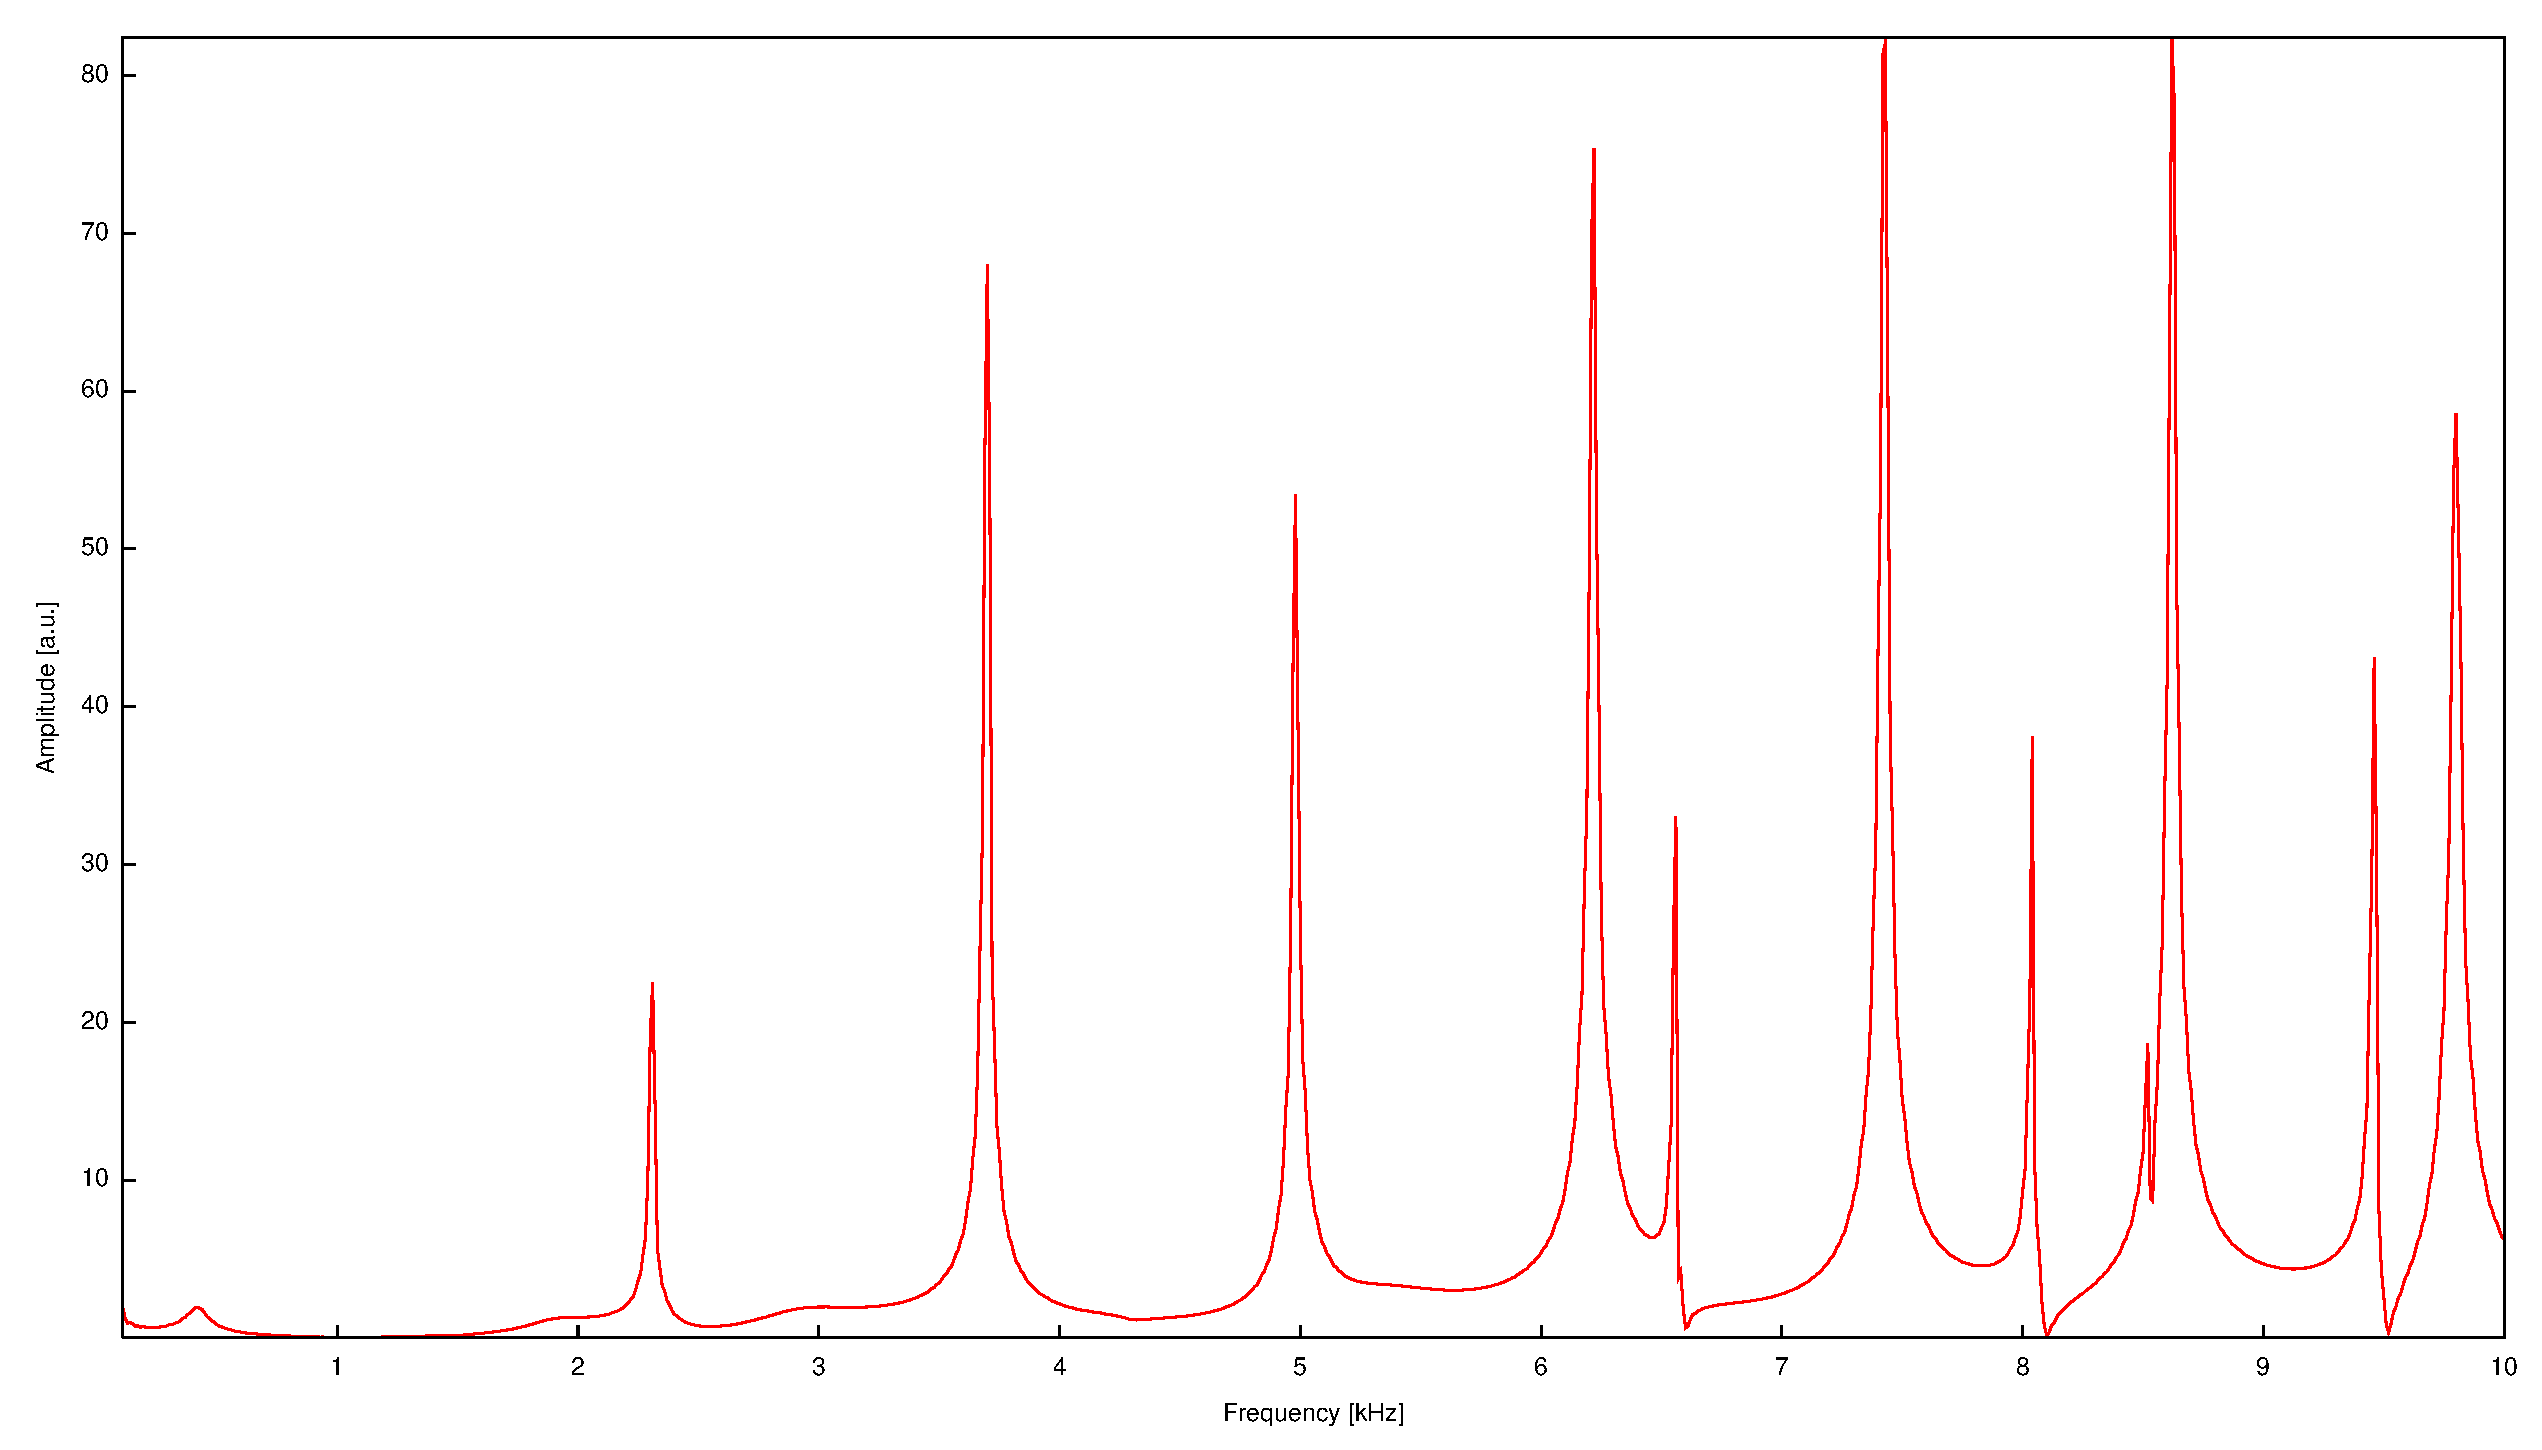
\includegraphics[width=\linewidth-60pt,height=\textheight-60pt,keepaspectratio]{FP-V23data/2.1_180degree.eps}
\caption{Spektrum im sphärischen Resonator für $\alpha=\SI{180}{\degree}$.}
\label{fig:Overview2}
\end{figure}

\begin{figure}
\centering
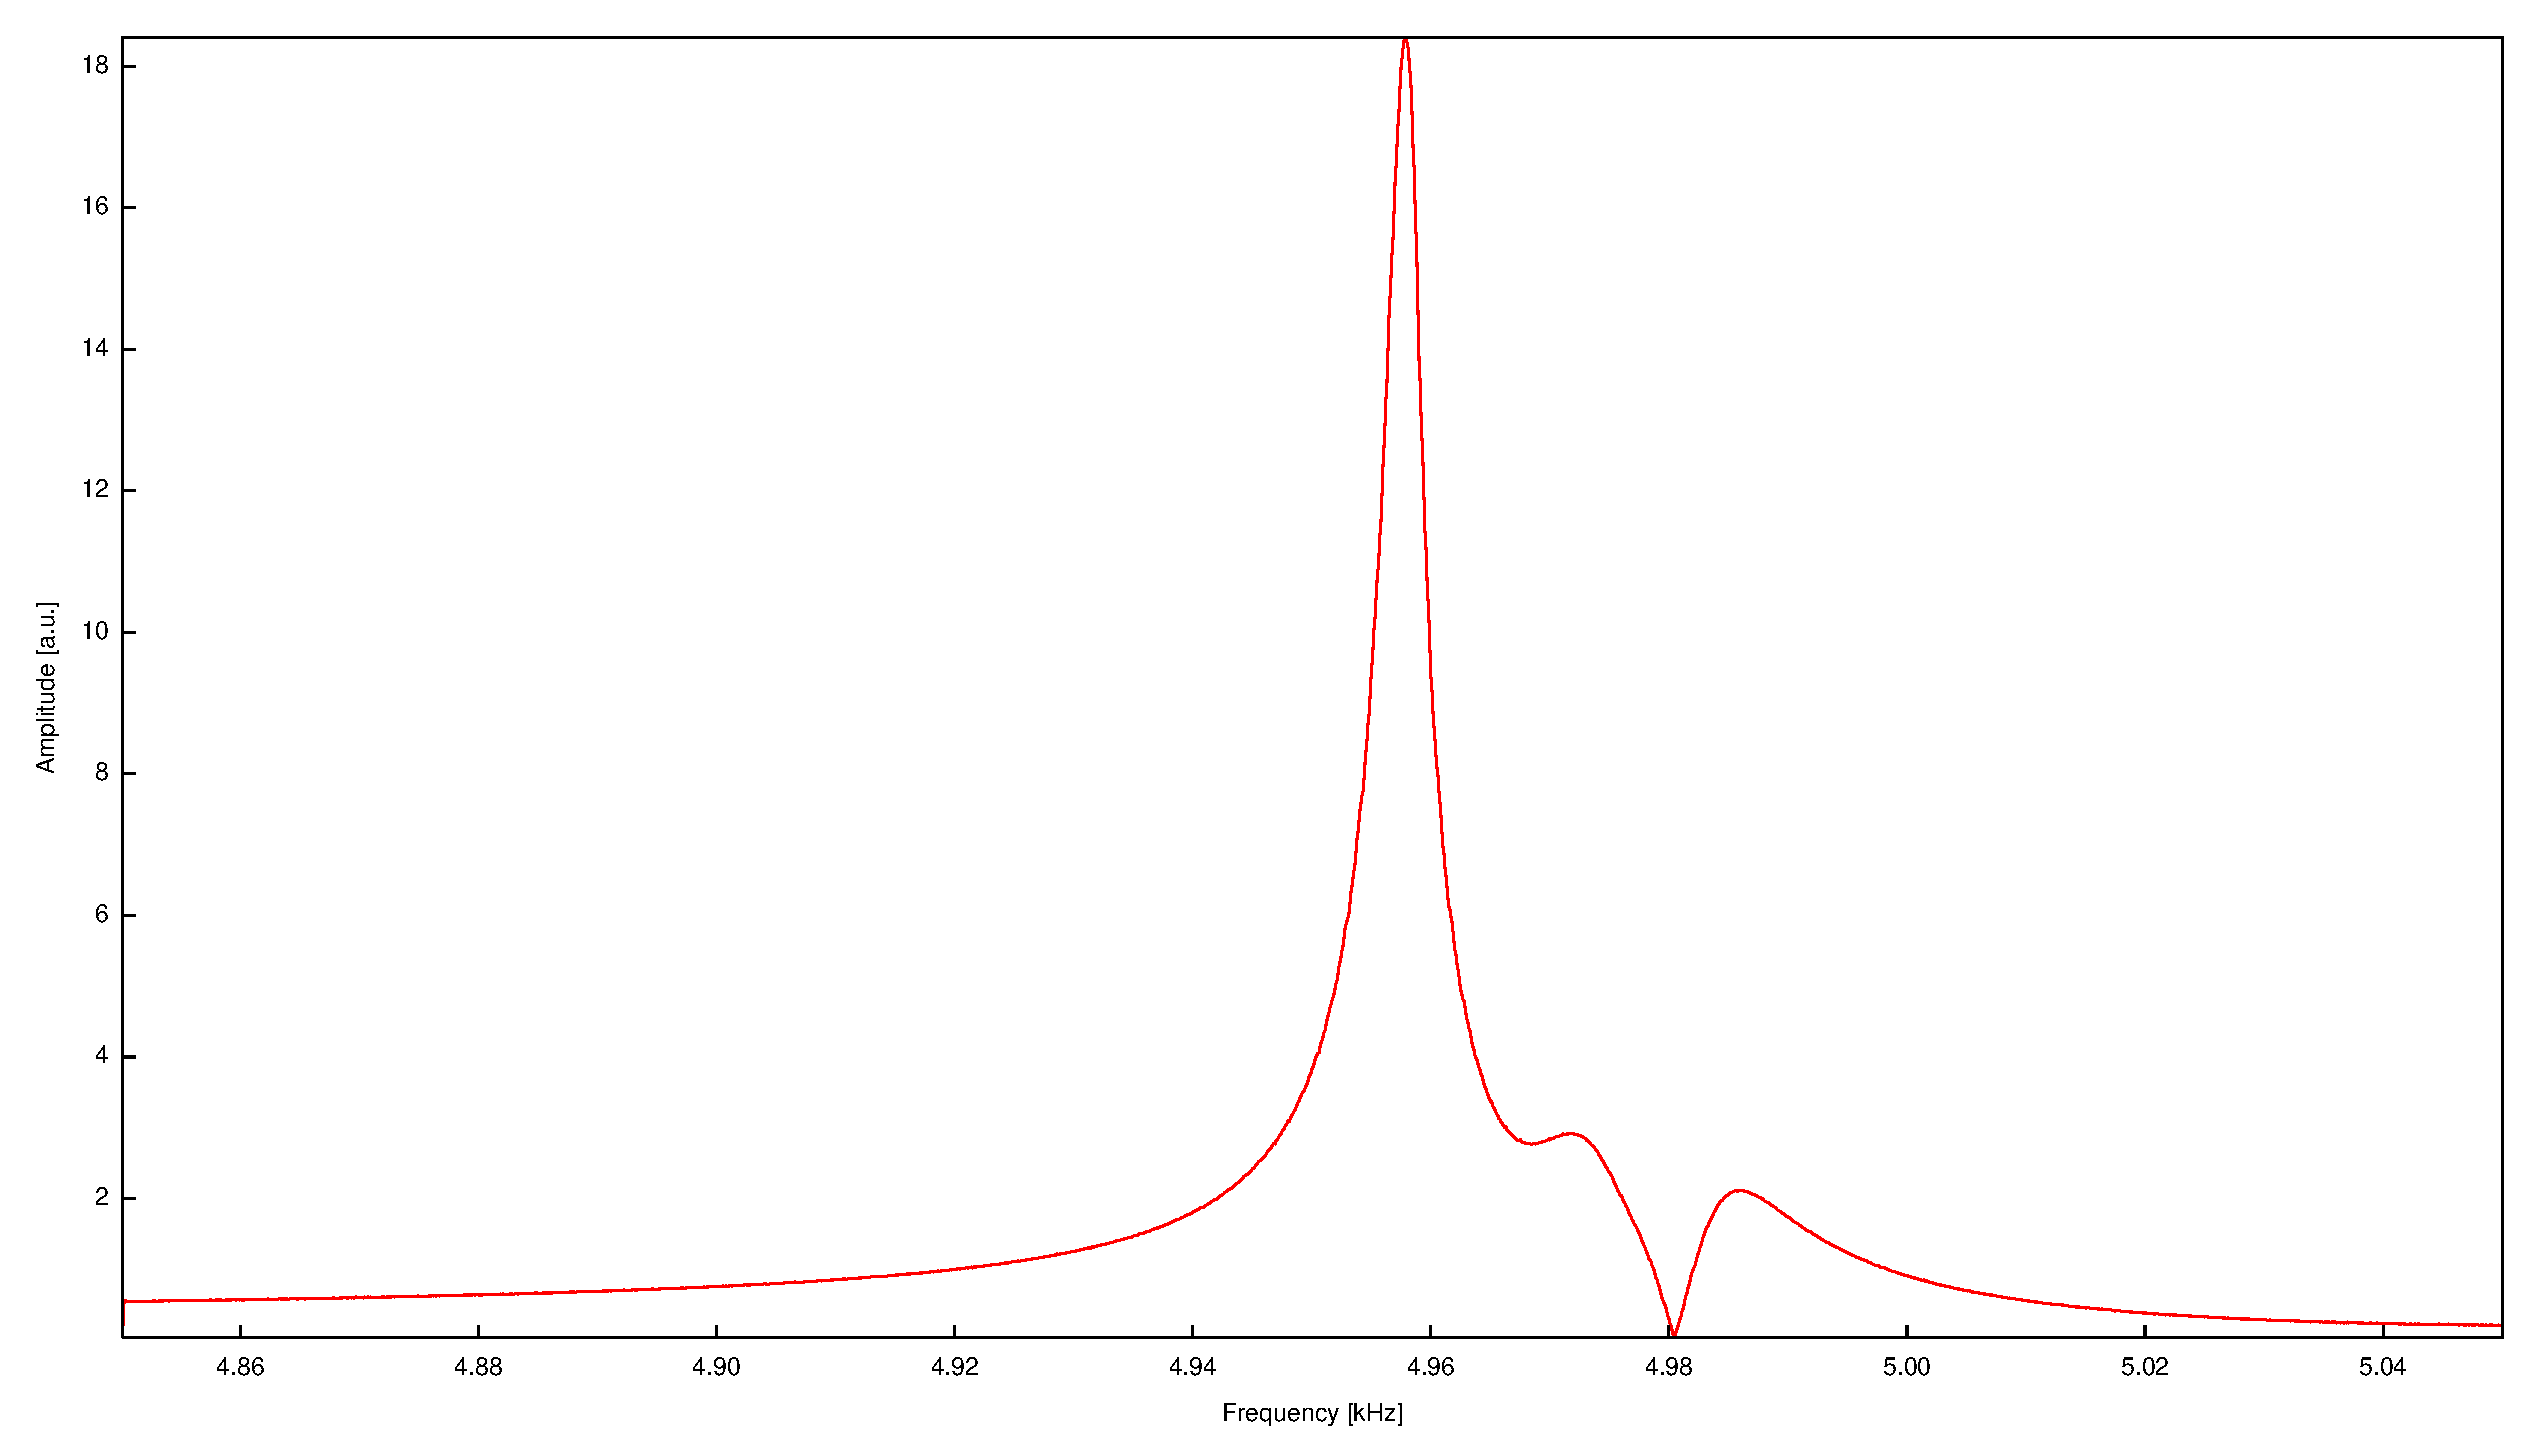
\includegraphics[width=\linewidth-60pt,height=\textheight-60pt,keepaspectratio]{FP-V23data/2.2_0degree.eps}
\caption{Nähere Aufnahme des Peaks bei $f\approx\SI{5000}{\hertz}$ für $\alpha=\SI{0}{\degree}$.}
\label{fig:5k_Peak1}
\end{figure}

\begin{figure}
\centering
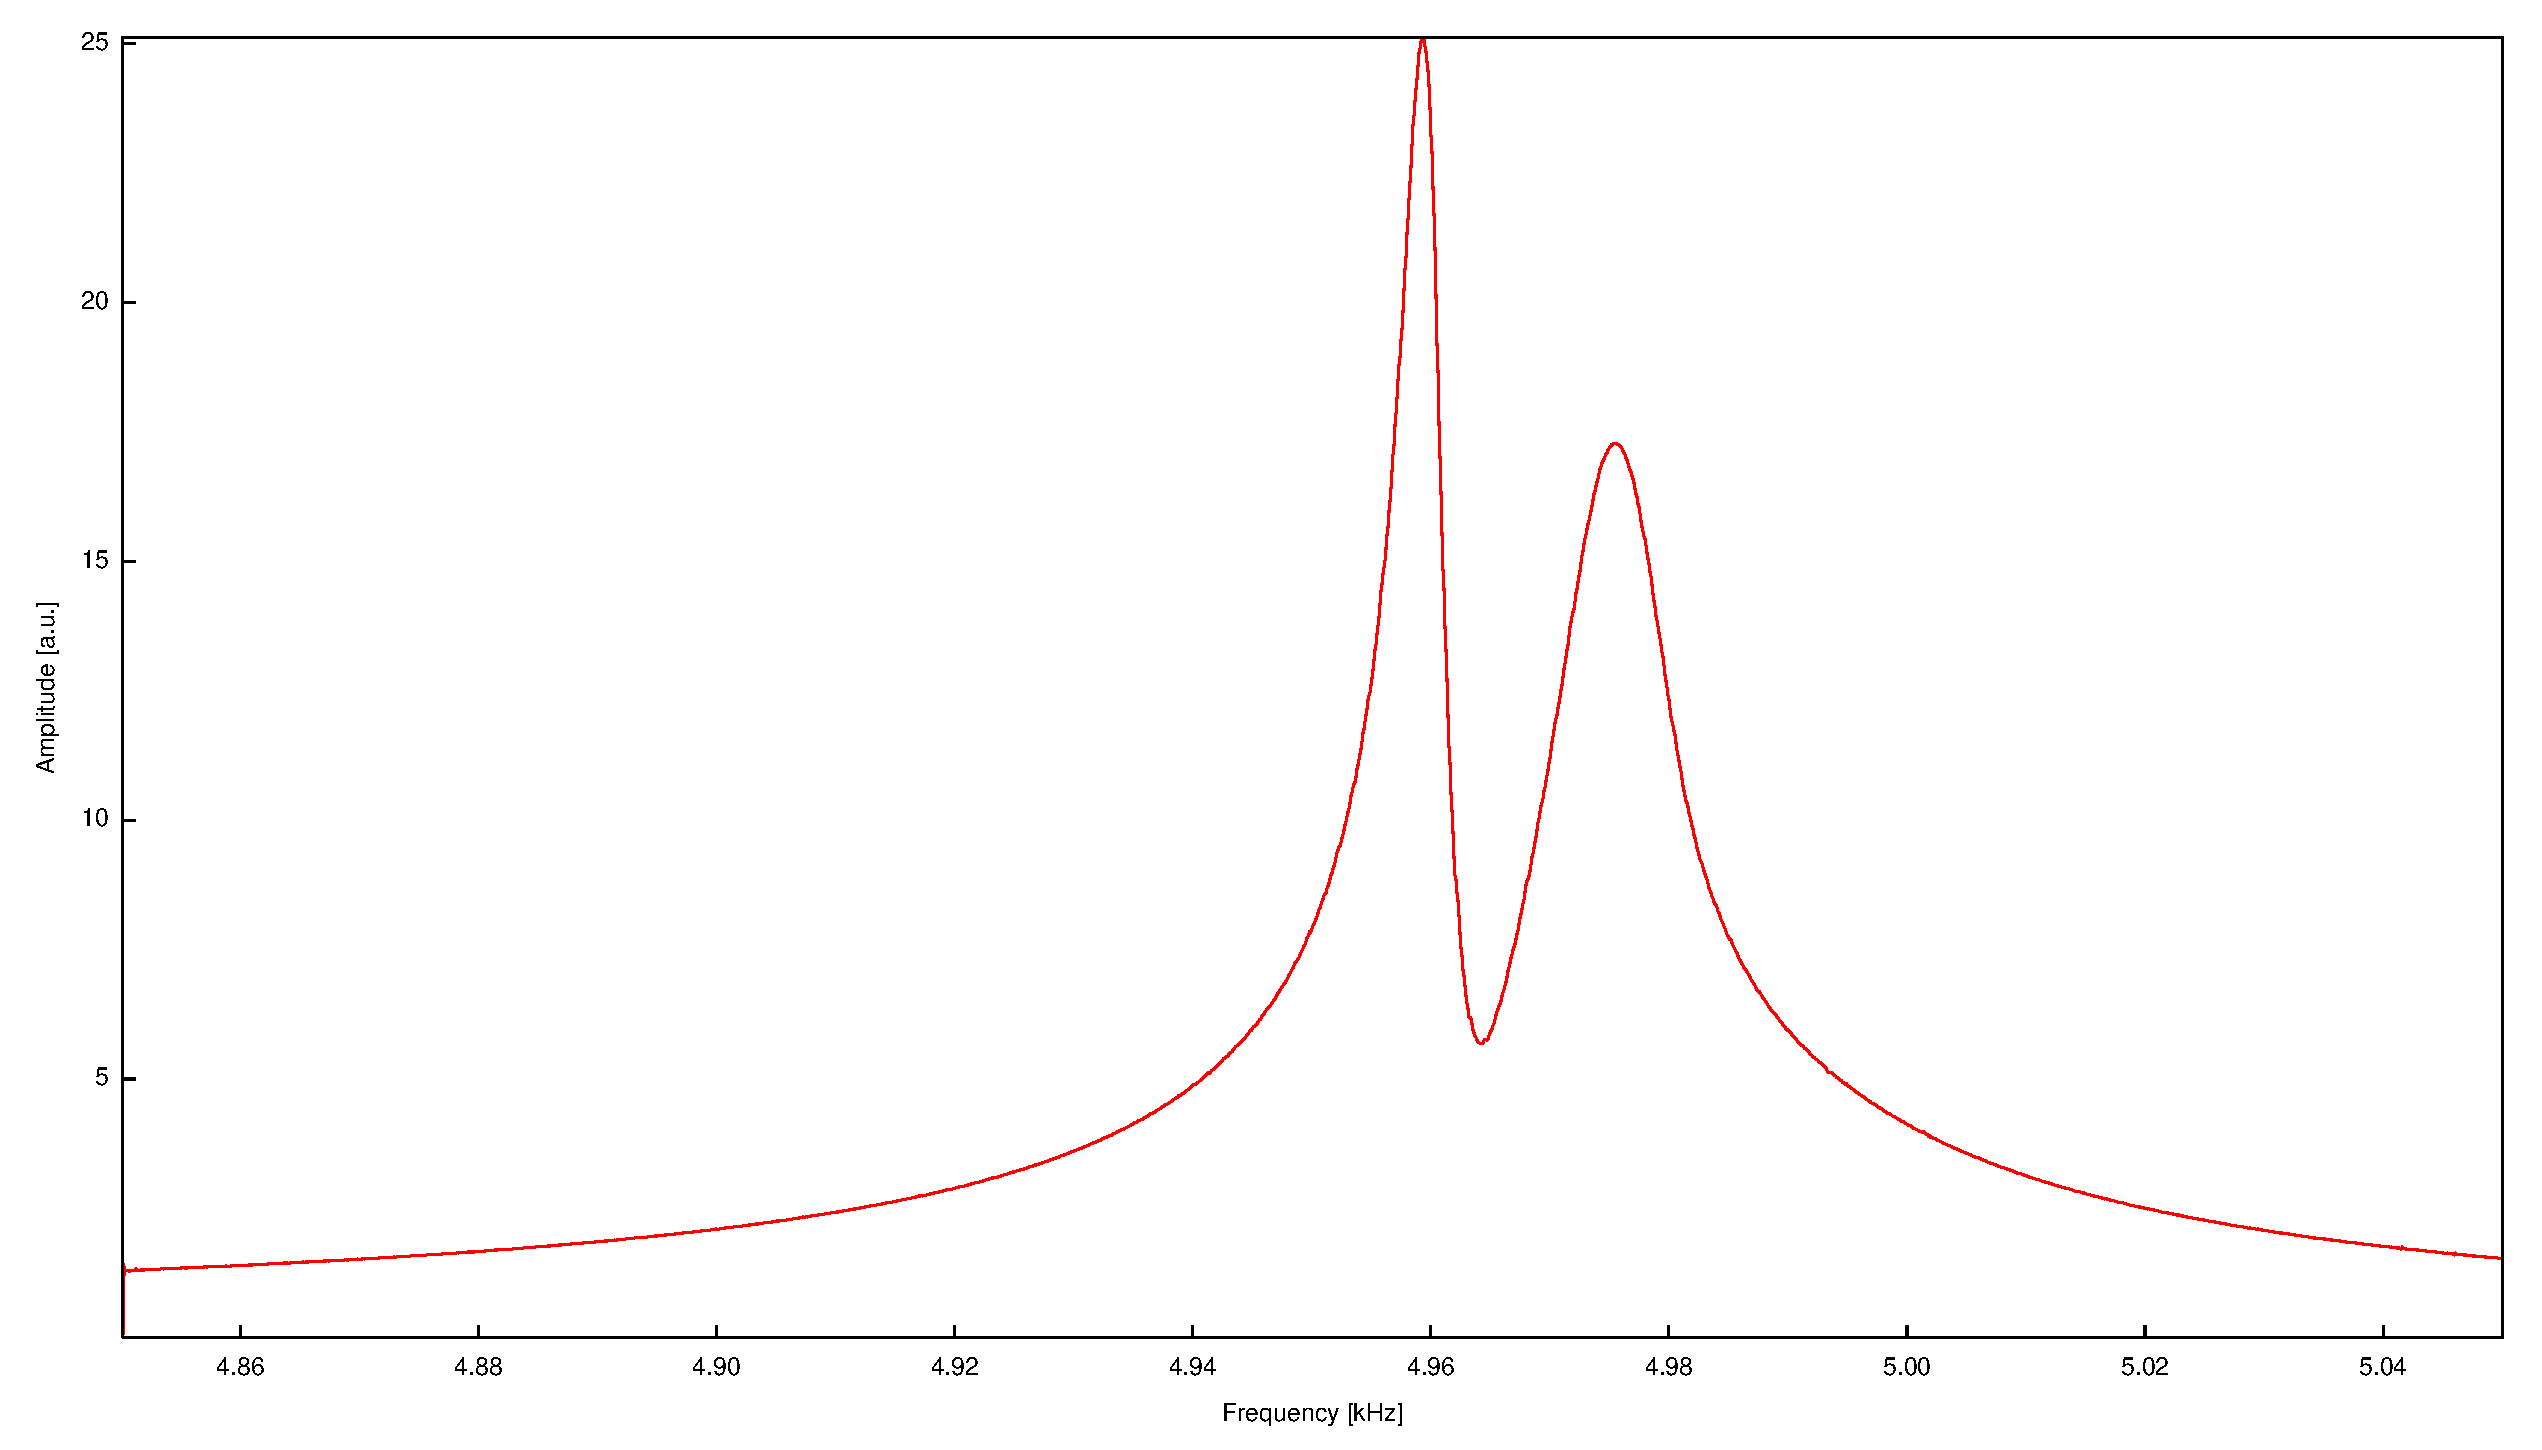
\includegraphics[width=\linewidth-60pt,height=\textheight-60pt,keepaspectratio]{FP-V23data/2.2_40degree.eps}
\caption{Nähere Aufnahme des Peaks bei $f\approx\SI{5000}{\hertz}$ für $\alpha=\SI{40}{\degree}$.}
\label{fig:5k_Peak2}
\end{figure}

\begin{figure}
\centering
\begin{minipage}{0.45\textwidth}
\centering
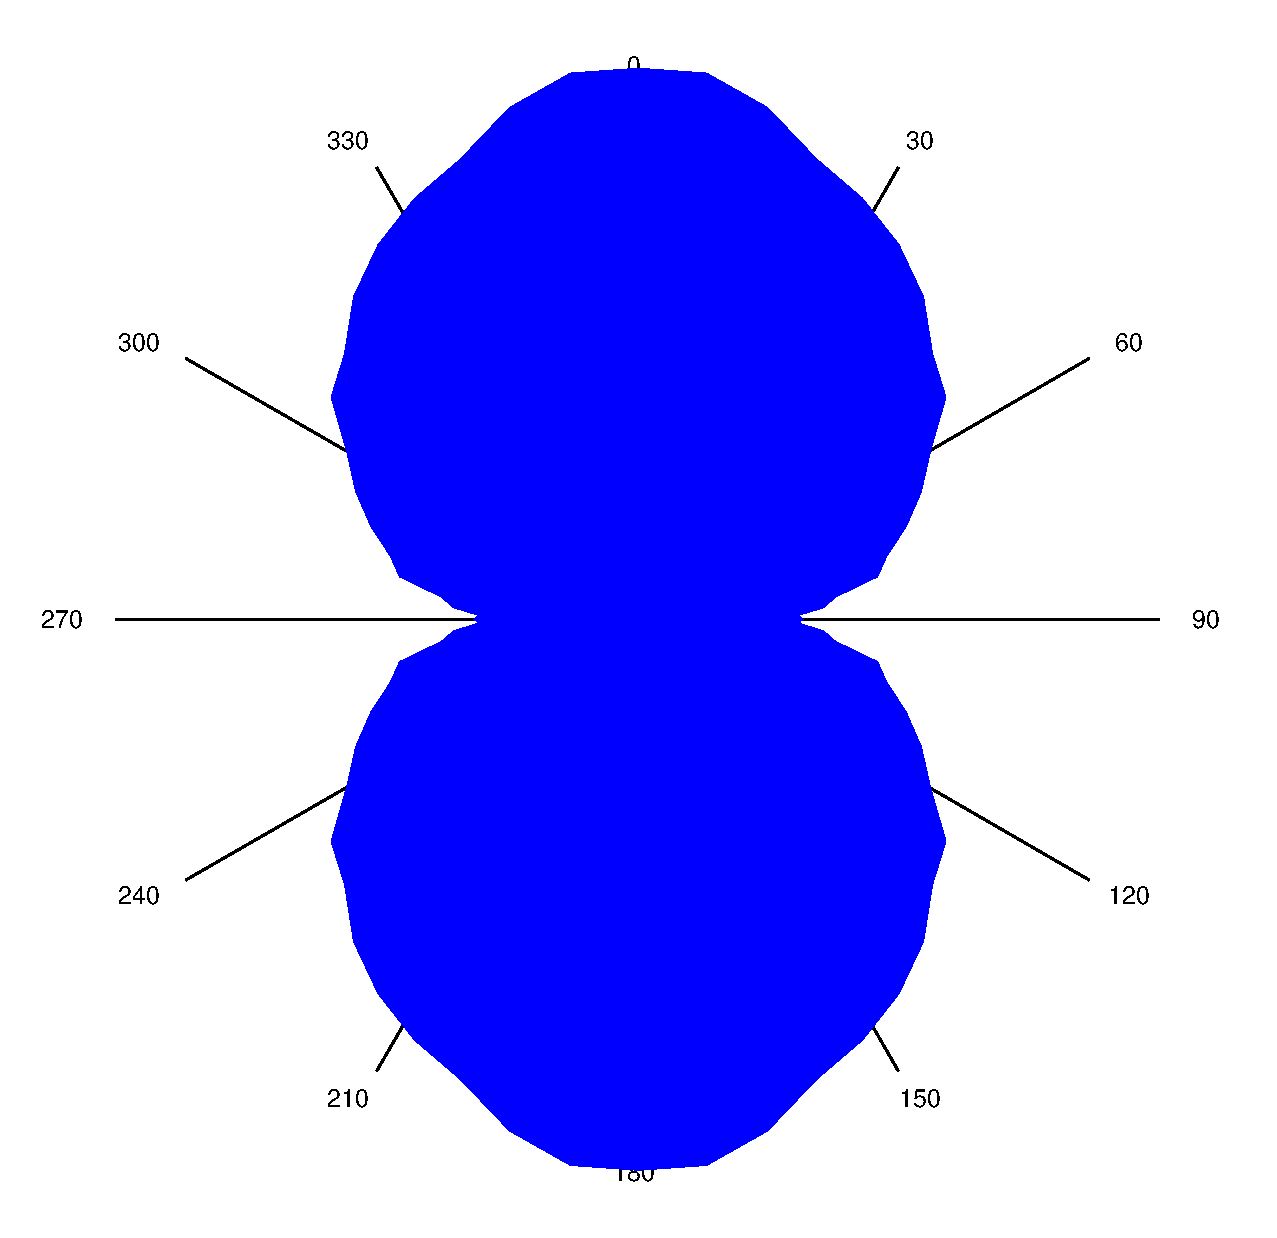
\includegraphics[width=\linewidth,keepaspectratio]{FP-V23data/2.3_2306.535Hz.eps}
%
(a) erster Peak bei $\SI{2307}{\hertz}$, $Y_1^0$.
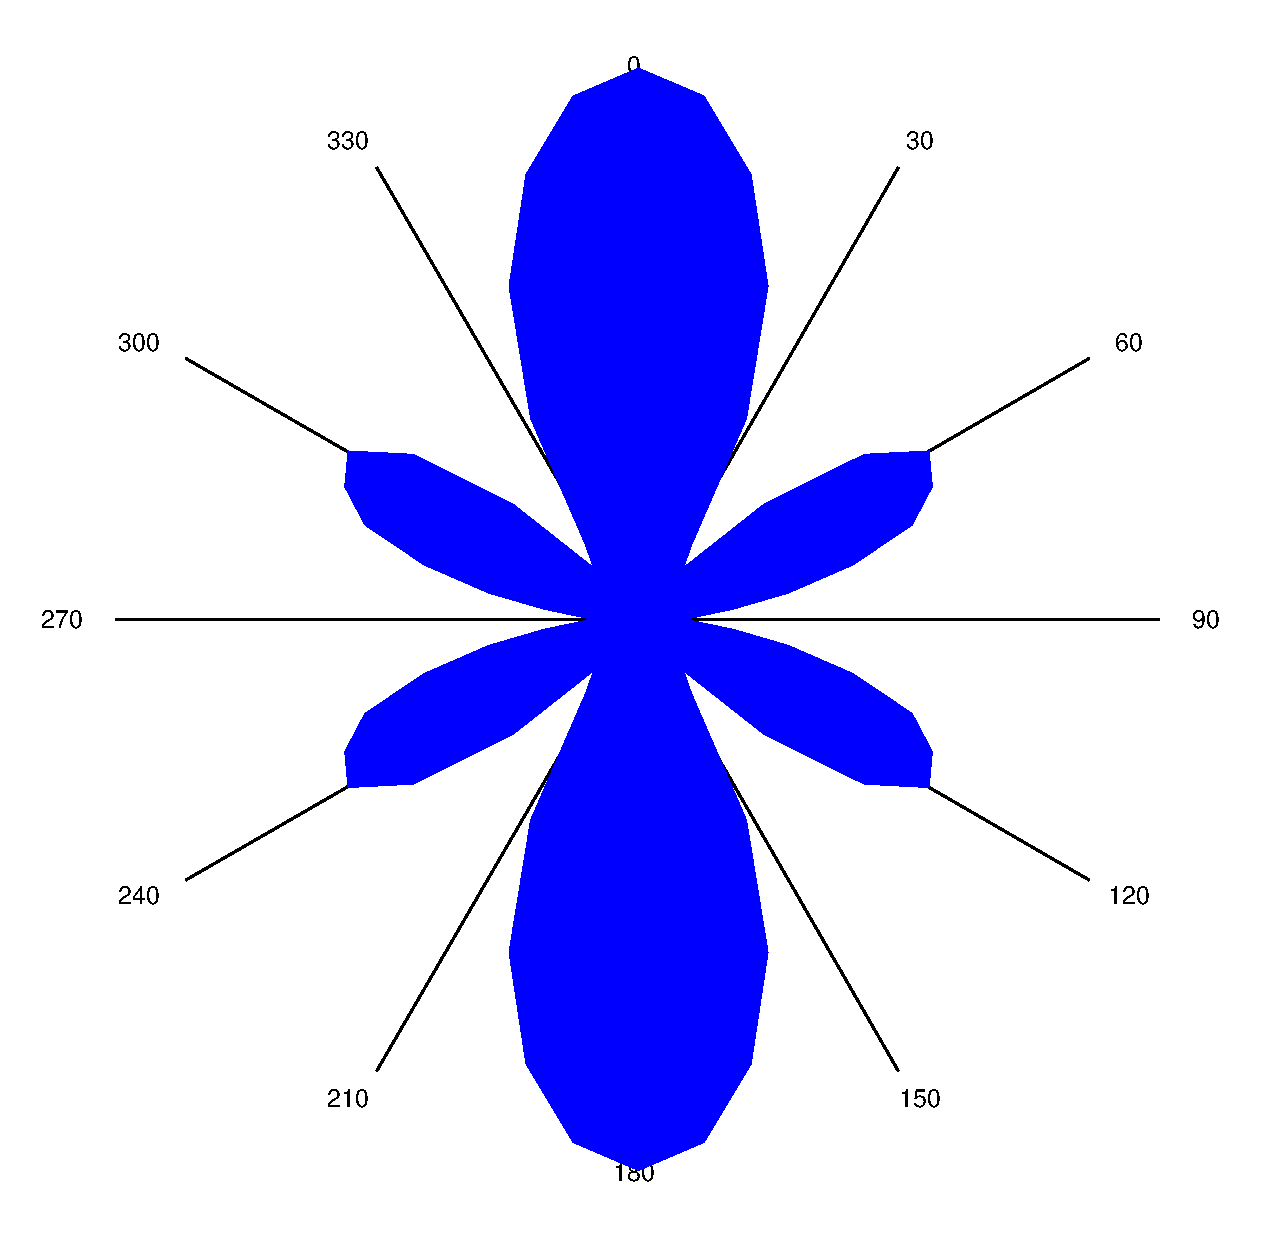
\includegraphics[width=\linewidth,keepaspectratio]{FP-V23data/2.3_4985.394Hz.eps}
%
(c) dritter Peak bei $\SI{4985}{\hertz}$, $Y_3^0$.
\end{minipage}
\begin{minipage}{0.45\textwidth}
\centering
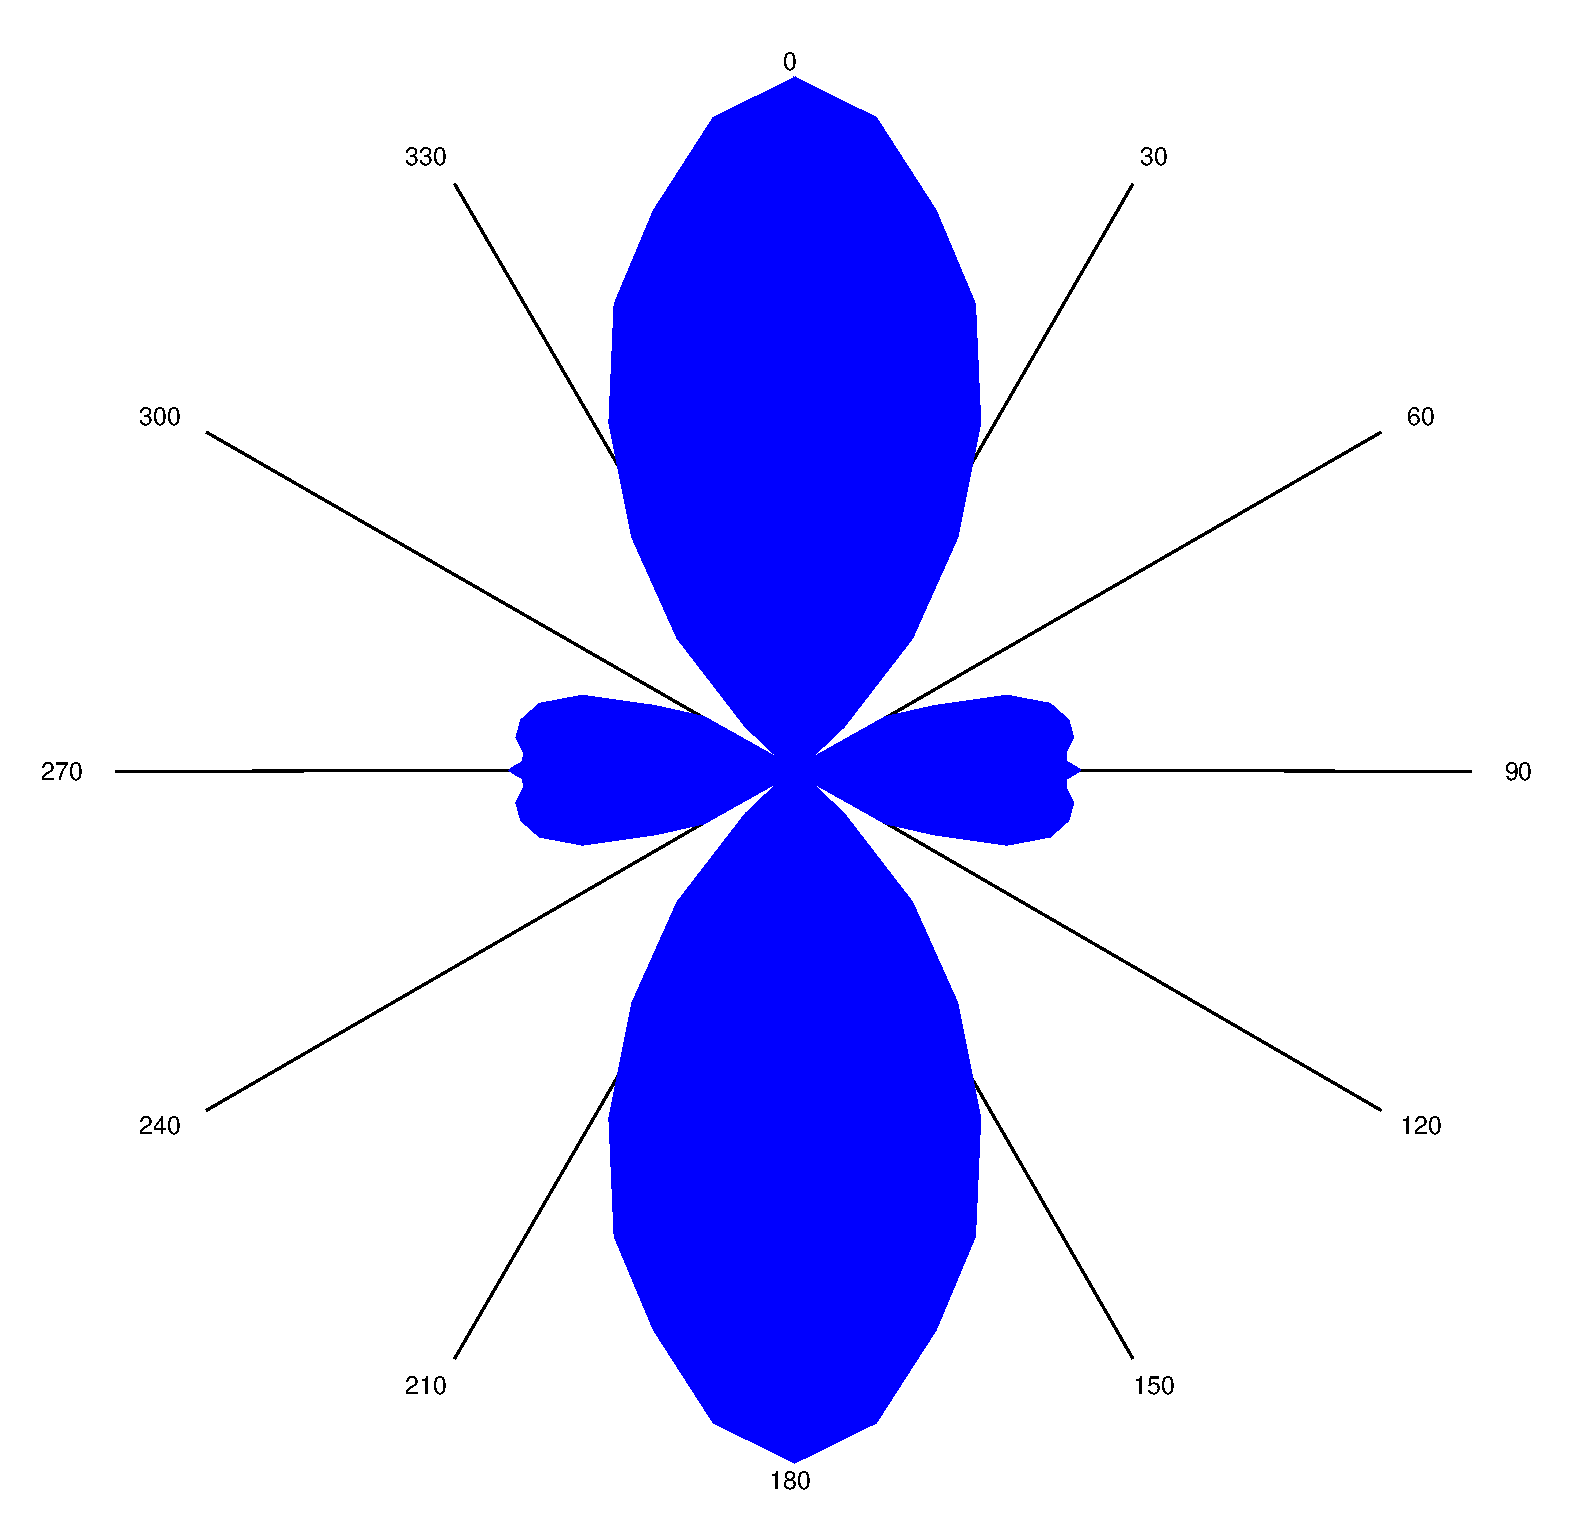
\includegraphics[width=\linewidth,keepaspectratio]{FP-V23data/2.3_3704.961Hz.eps}
%
(b) zweiter Peak bei $\SI{3705}{\hertz}$, $Y_2^0$.
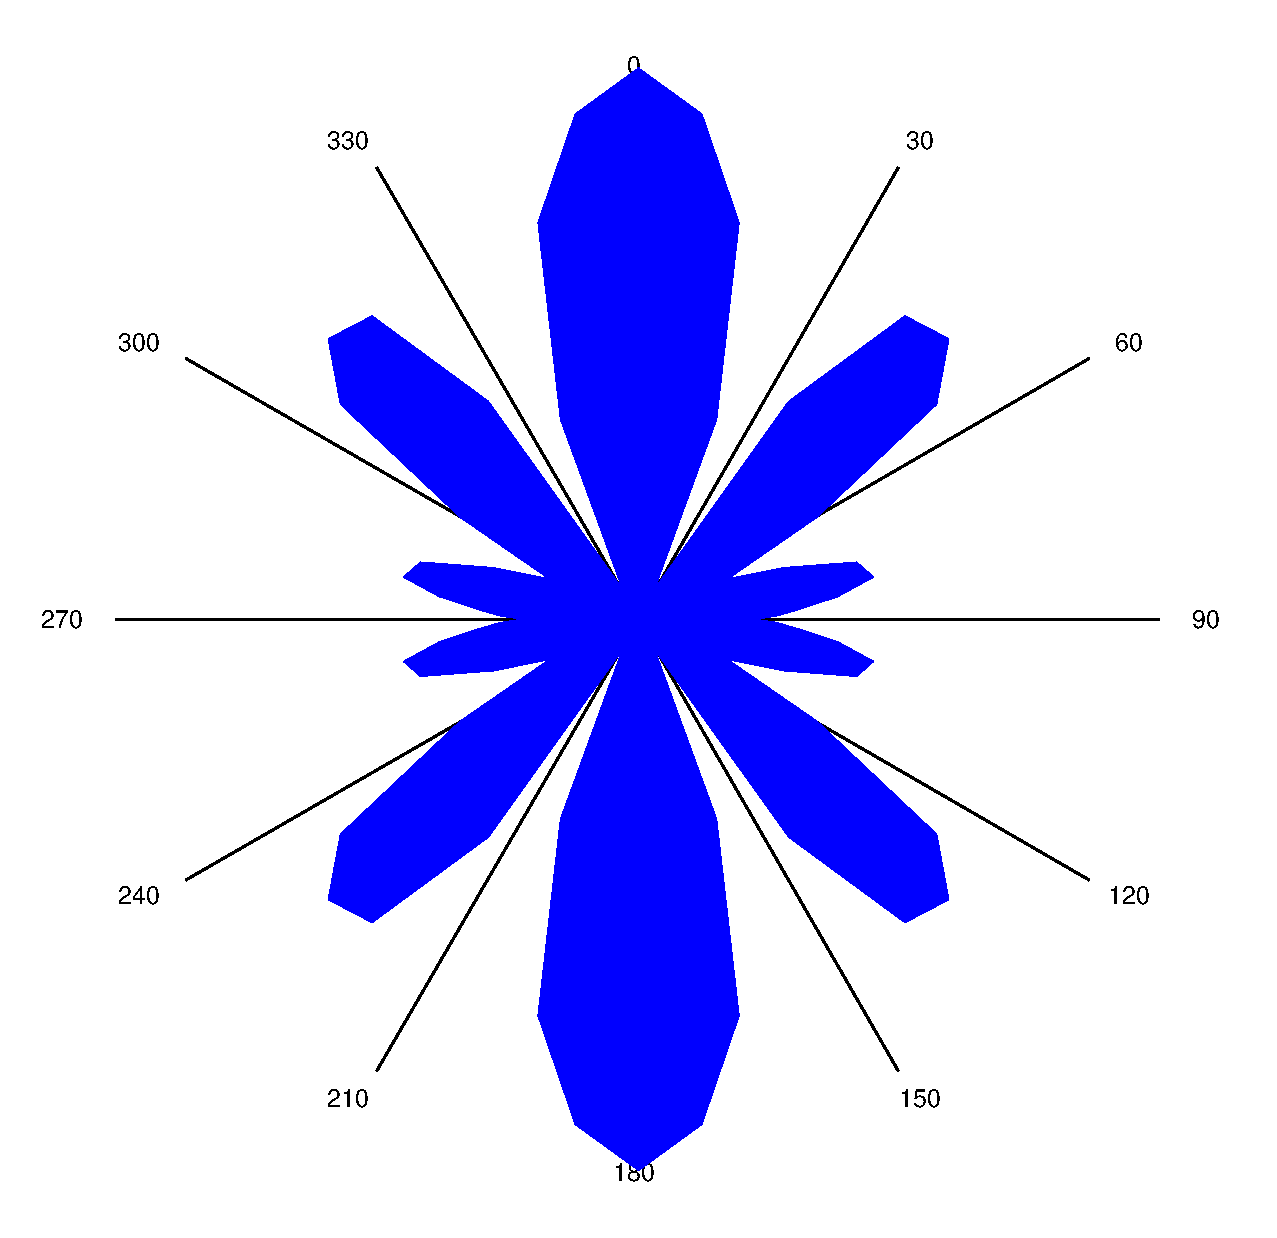
\includegraphics[width=\linewidth,keepaspectratio]{FP-V23data/2.3_6230.866Hz.eps}
%
(d) vierter Peak bei $\SI{6231}{\hertz}$, $Y_4^0$.
\end{minipage}
\begin{minipage}{\textwidth}
\centering
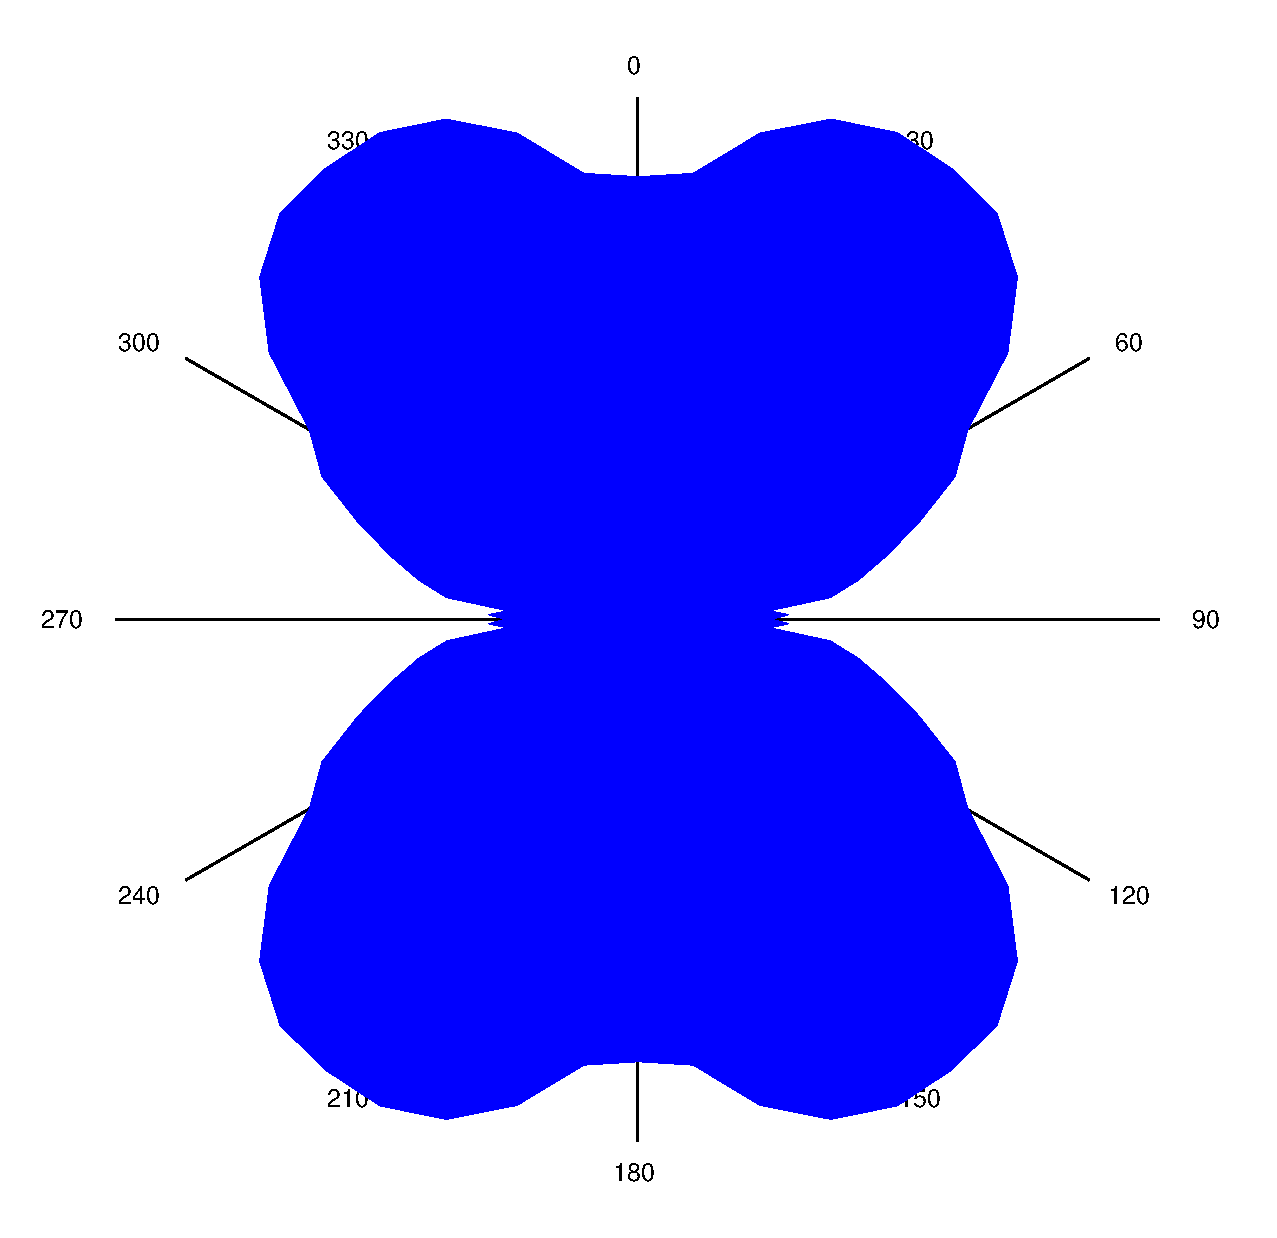
\includegraphics[width=\linewidth*9/20,keepaspectratio]{FP-V23data/2.3_6571.732Hz.eps}

%
(e) fünfter Peak bei $\SI{6571}{\hertz}$, eventuell $Y_2^1$.
\end{minipage}
\caption{Polarplots der ersten fünf Peaks im sphärischen Resonator}
\label{fig:polar}
\end{figure}

\subsection{Modellierung: Ein eindimensionaler Festkörper}
\subsubsection{Teilchen im periodischen Potential}

In Abbildung \ref{fig:Spek4_1} ist beispielhaft das Spektrum von  $\SI{5000}{\hertz}$ bis $\SI{14000}{\hertz}$ einer $\SI{75}{\milli\meter}$-Röhre zu sehen.
Der mittlere Abstand zwischen den Peaks wird über die Formel zur Berechnung des Mittelwerts
\[
\mu_{\Delta f} = \frac{1}{N}\sum_{i=1}^{N}(\Delta f)_i
\]
und dessen Standardabweichung
\[
\sigma_{\Delta f} = \sqrt{\frac{1}{N(N-1)}\sum_{i=1}^{N}((\Delta f)_i-\mu_{\Delta f})^2}
\]
bestimmt. Dasselbe wird für zwei bis acht $\SI{75}{\milli\meter}$-Röhren durchgeführt. Die berechneten Mittelwerte sind in Tabelle
\ref{tab:mu} zu sehen und sind in Abbildung \ref{fig:Df_L} gegen das Inverse der Röhrenlänge $L$ aufgetragen. Eine nicht gewichtete lineare Ausgleichsrechnung der Form 
\[
\Delta f\left(\frac{1}{L}\right)= a\cdot\frac{1}{L}+b
\]
liefert die Parameter
\begin{align*}
a&=\SI{169,81(20)}{\meter\per\second}\\
b&=\SI{5,7(12)}{\second^{-1}}\text{.}
\end{align*}
Ein Koeffizientenvergleich mit Gleichung \eqref{eq:f} liefert für die Schallgeschwindigkeit $c$ die Beziehung
\[
c=2 a=\SI{339,6(4)}{\meter\per\second}\text{.}
\]

\begin{figure}
\centering
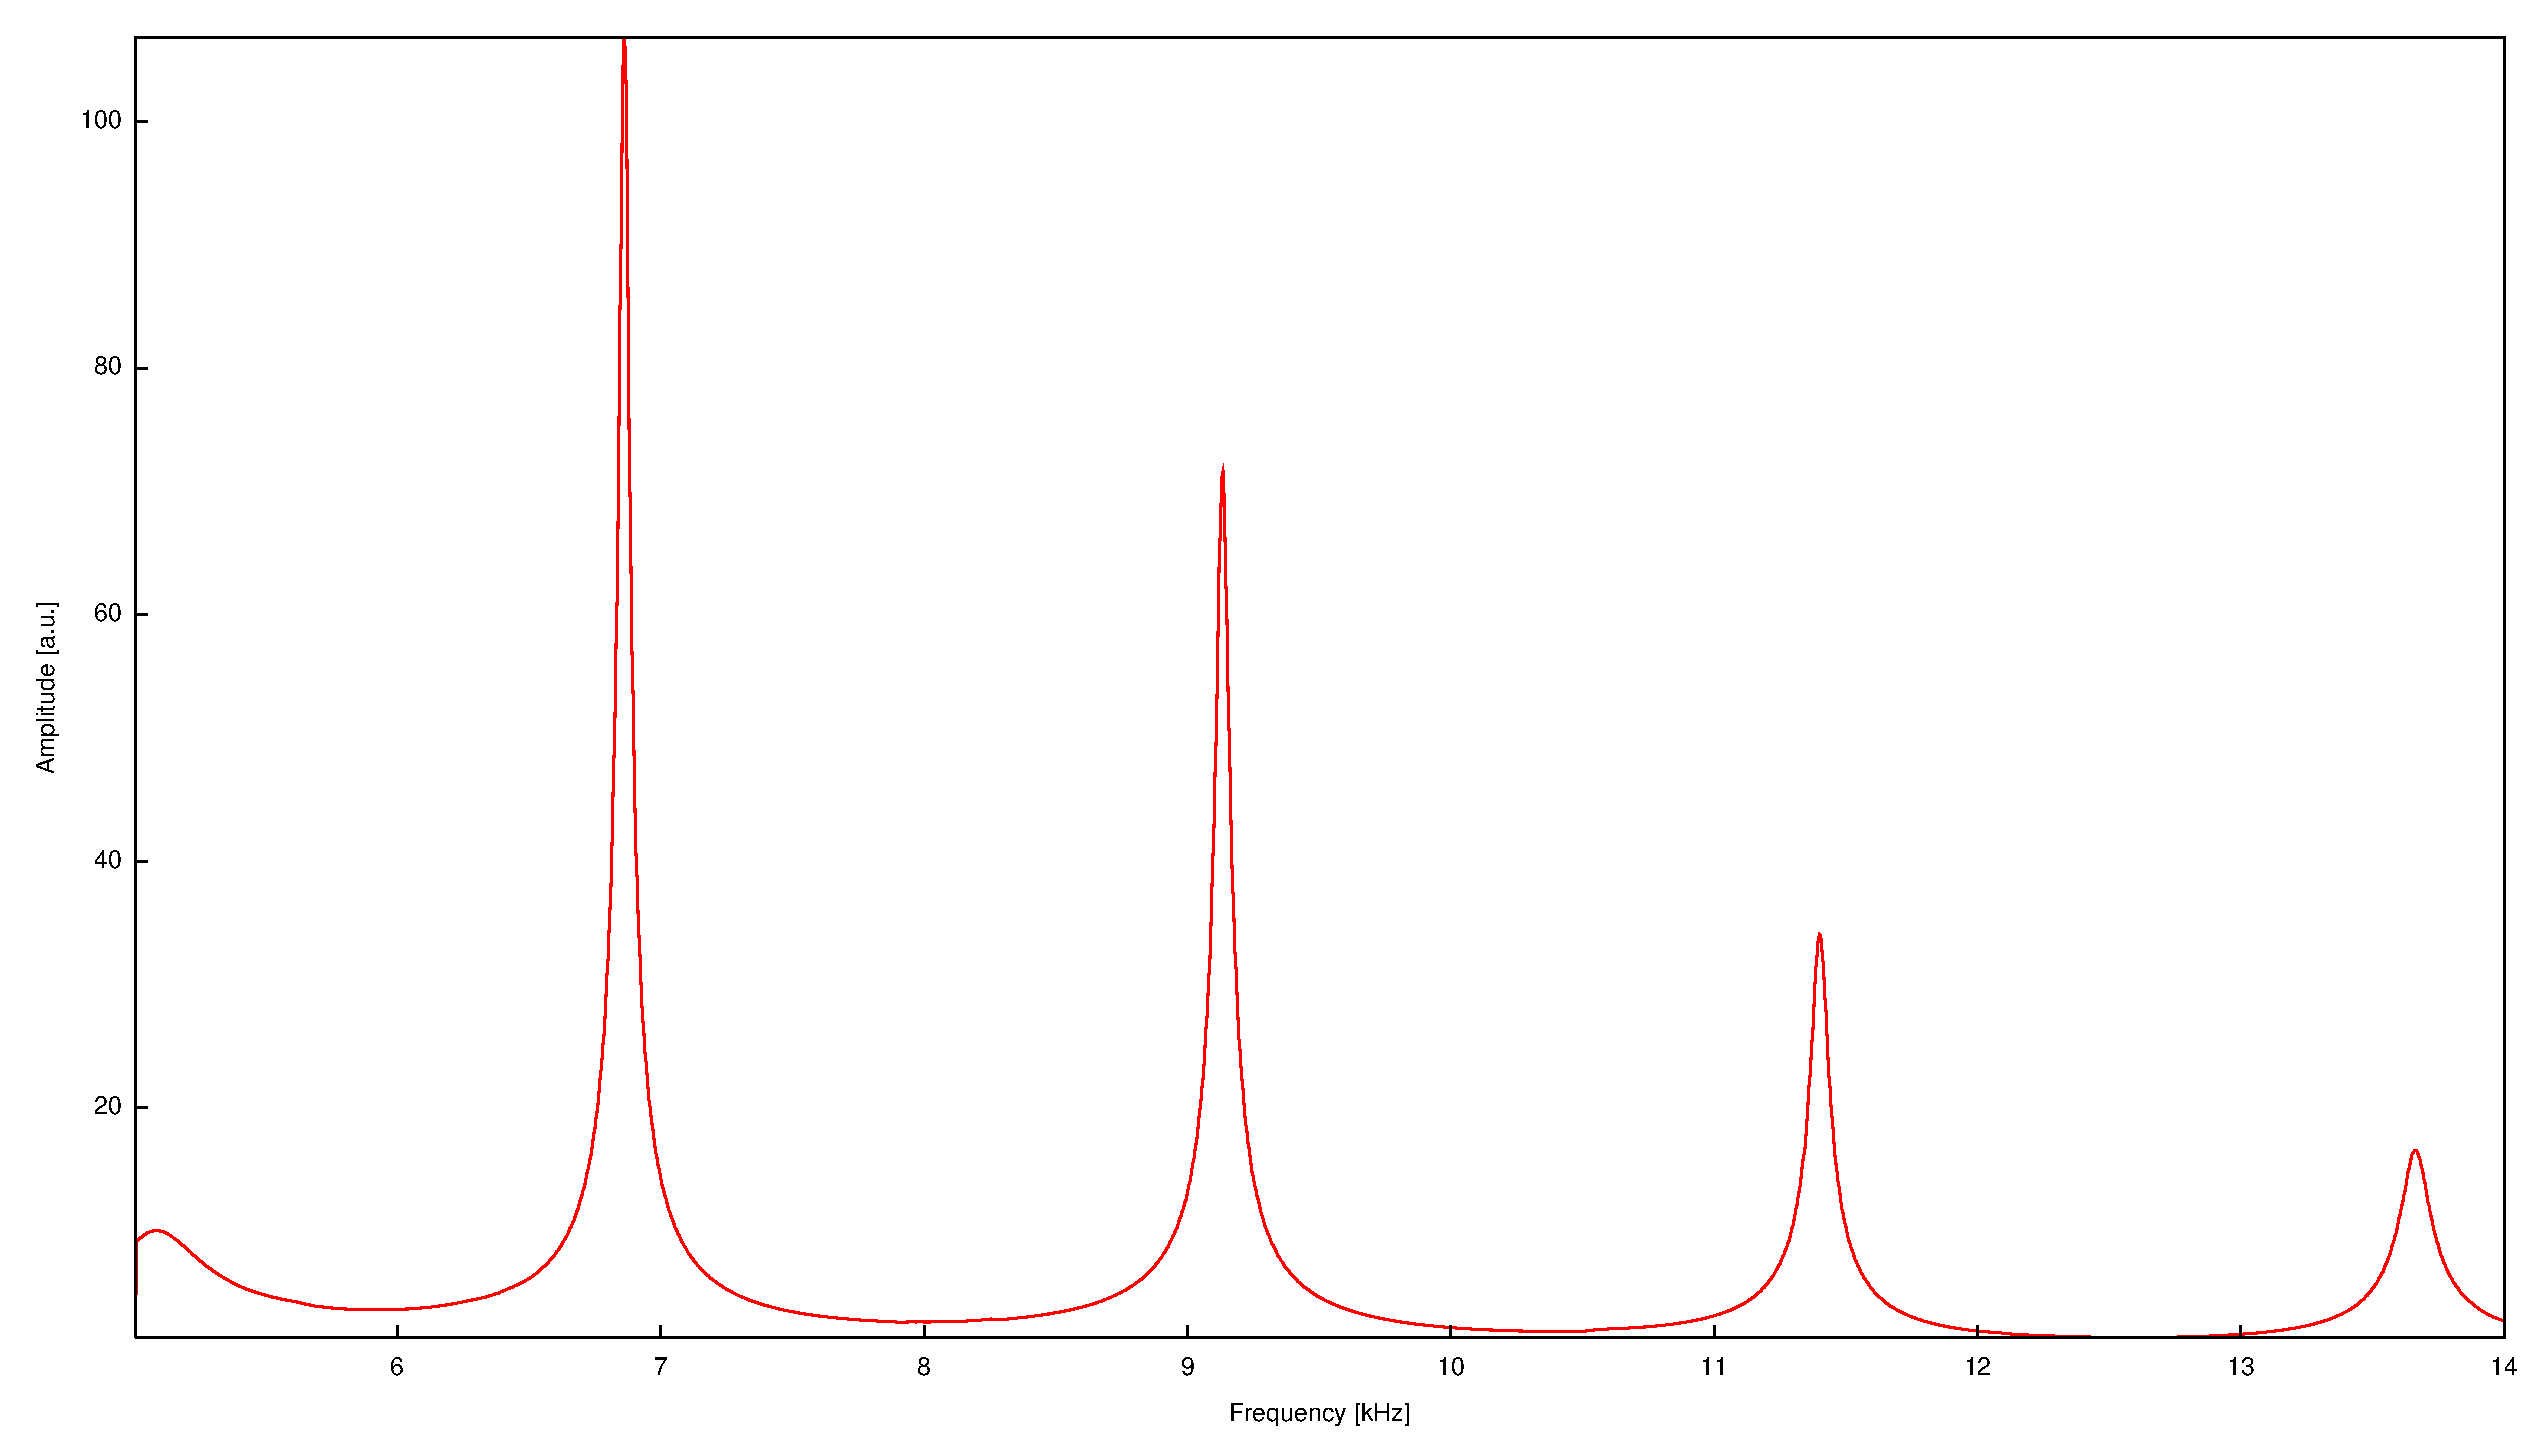
\includegraphics[width=\linewidth-60pt,height=\textheight-60pt,keepaspectratio]{FP-V23data/4.1_75mm.eps}
\caption{Spektrum von einer $\SI{75}{\milli\meter}$-Röhre.}
\label{fig:Spek4_1}
\end{figure}

\begin{table}
\caption{Mittlerer Abstand der Peaks.}
\centering
\label{tab:mu}
	\sisetup{table-format=1.2}
	\begin{tabular}{S[table-format=3.0]r@{${}\pm{}$}l}
		\toprule
		{$L/(\si{\milli\meter})$} & \multicolumn{2}{c}{$\Delta f/(\si{\second^{-1}})$} \\
		\midrule
		 75 & 2268.3 & 3.3 \\
		 150 & 11393 & 2.5 \\
		 225 & 763.3 & 1.4 \\
		 300 & 573.5 & 1.3 \\
		 375 & 458.6 & 1.2 \\
		 450 & 382.7 & 0.9 \\
		 525 & 327.1 & 0.7 \\
		 600 & 286.6 & 0.6 \\
		\bottomrule
	\end{tabular}

\label{tab:mu}
\end{table}

\begin{figure}
\centering
\includegraphics[width=\linewidth-60pt,height=\textheight-60pt,keepaspectratio]{build/4.1.pdf}
\caption{$\Delta f$ aufgetragen gegen $\frac{1}{L}$ zur Bestimmung der Schallgeschwindigkeit $c$.}
\label{fig:Df_L}
\end{figure}

\newpage
\noindent In Abbildung \ref{fig:12_50} ist das Spektrum von zwölf $\SI{50}{\milli\meter}$-Röhren zu sehen und in Abbildung \ref{fig:w_k} werden als Dispersionsrelation die Winkelfrequenzen der Peaks $\omega_n=2\pi f_n$ gegen die zugehörigen Wellenzahlen $k_n$ aufgetragen. Eine lineare Ausgleichsrechnung der Form $\omega(k)=m k + n$ liefert die Parameter
\begin{align*}
m&=\SI{343,77(16)}{\meter\per\second}\\
n&=\SI{156(21)}{\second^{-1}}\text{.}
\end{align*}
Ein Vergleich mit Gleichung \eqref{eq:w_k} zeigt das $m=c$ der Schallgeschwindigkeit entspricht.\\

\begin{figure}
\centering
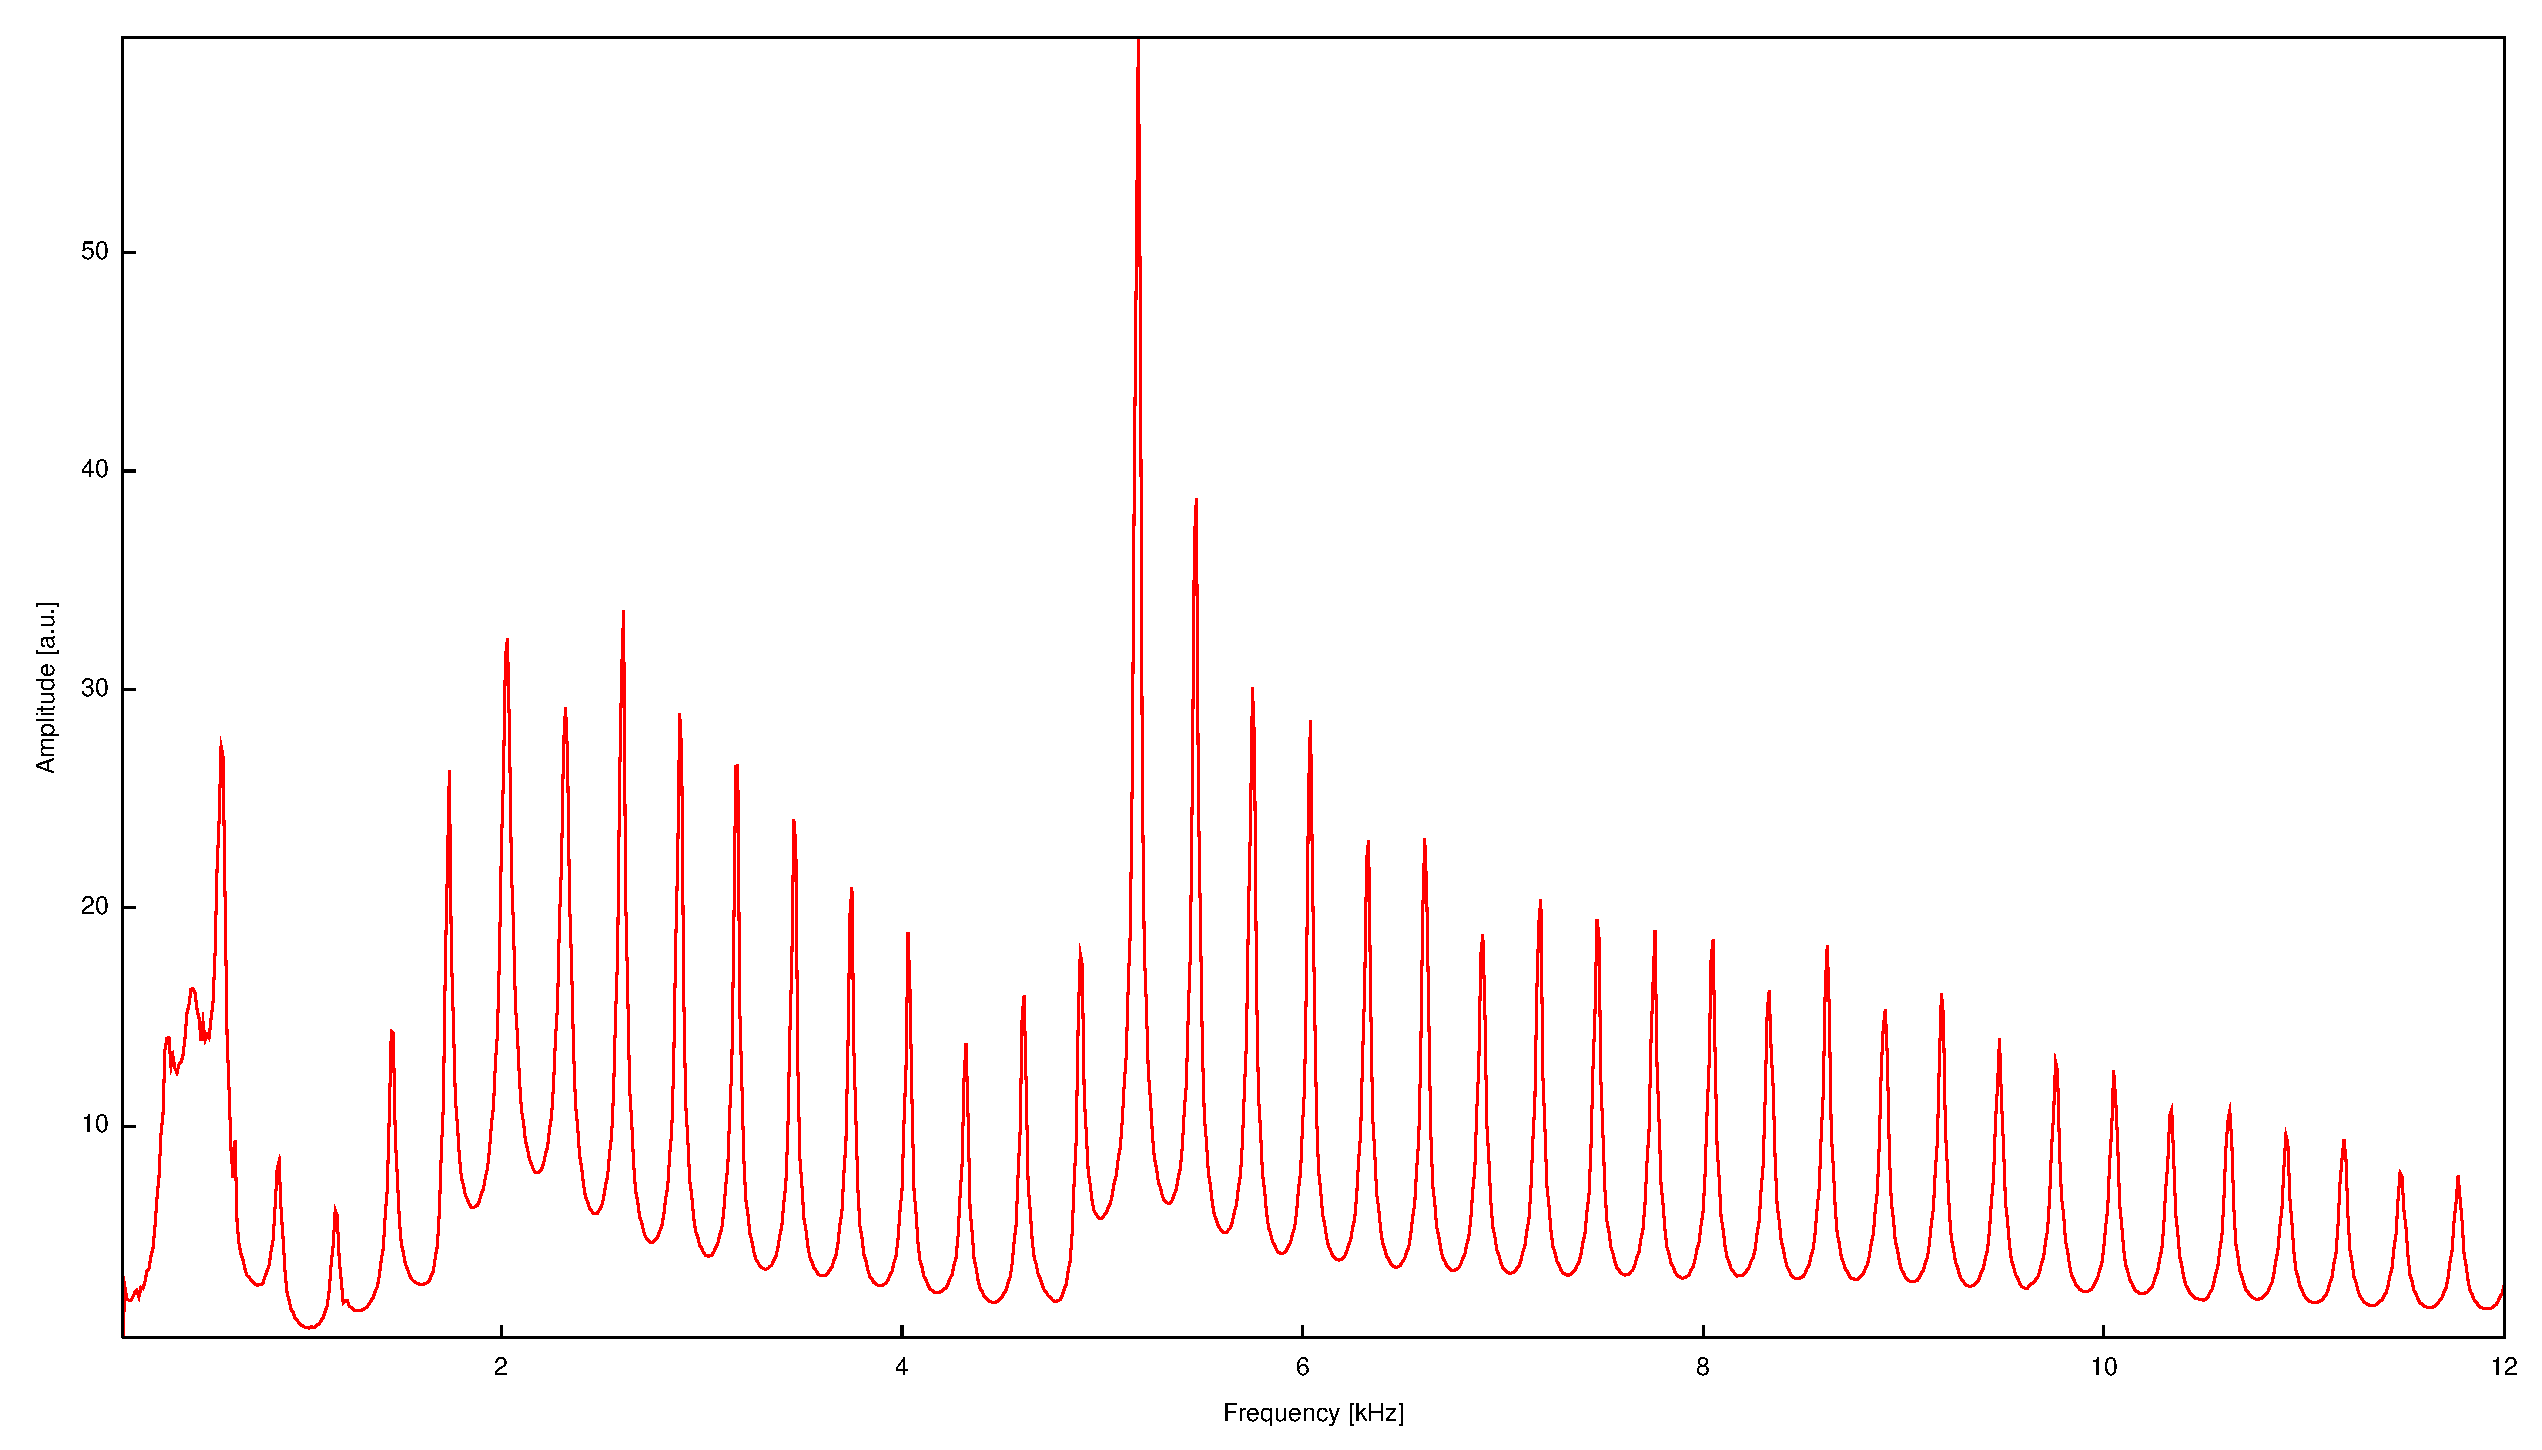
\includegraphics[width=\linewidth-60pt,height=\textheight-60pt,keepaspectratio]{FP-V23data/4.2_600mm.eps}
\caption{Spektrum von zwölf $\SI{50}{\milli\meter}$-Röhren.}
\label{fig:12_50}
\end{figure}

\begin{figure}
\centering
\includegraphics[width=\linewidth-60pt,height=\textheight-60pt,keepaspectratio]{build/4.2.pdf}
\caption{Dispersionsrelation $\omega(k)$ von zwölf $\SI{50}{\milli\meter}$-Röhren}
\label{fig:w_k}
\end{figure}

\newpage
\noindent In Abbildung \ref{fig:8_50_16} ist das Spektrum von acht über $\SI{16}{\milli\meter}$-Iriden gekoppelten $\SI{50}{\milli\meter}$-Röhren zu sehen. Dieselbe Messung wird für $10$- und $\SI{13}{\milli\meter}$-Kopplungen durchgeführt und die jeweiligen Dispersionsrelationen in den Abbildungen \ref{fig:w_k_1} bis \ref{fig:w_k_3} aufgetragen.\\
In Tabelle \ref{tab:band} sind die Breiten der Bänder und Bandlücken zu sehen. Es ist zu erkennen, dass bei abnehmendem Irisdurchmesser die Bänder schmaler werden, während die Breite der Bandlücken zunimmt. Die Fehler auf die Breite sind bedingt durch die gewählte Schrittweite von $\SI{10}{\hertz}$ und werden linear addiert. Da die Frequenz als $\omega = 2\pi f$ angegeben wird ist noch der Faktor $2\pi$ zu beachten.\\

\begin{table}
\caption{Breiten $b$ der Bänder und Bandlücken bei einem Irisdurchmesser von $\SI{10}{\milli\metre}$, $\SI{13}{\milli\metre}$ und $\SI{16}{\milli\metre}$.}
\centering
\label{tab:mu}
	\sisetup{table-format=1.2}
	\begin{tabular}{lS[table-format=2.2]@{${}\pm{}$}S[table-format=1.2]S[table-format=2.2]@{${}\pm{}$}S[table-format=1.2]S[table-format=2.2]@{${}\pm{}$}S[table-format=1.2]}
		\toprule
		{Band/Bandlücke} & \multicolumn{2}{c}{$b_{10}/\si{\kilo\hertz}$} & \multicolumn{2}{c}{$b_{13}/\si{\kilo\hertz}$} & \multicolumn{2}{c}{$b_{16}/\si{\kilo\hertz}$} \\
		\midrule
		 Band1  &  8,92 & 0,13 & 10,87 & 0,13 & 12,57 & 0,13\\
		 Band2  &  4,96 & 0,13 &  8,17 & 0,13 & 11,12 & 0,13\\
		 Band3  &  3,14 & 0,13 &  5,03 & 0,13 &  8,92 & 0,13\\
		 Band4  &  2,07 & 0,13 &  4,27 & 0,13 &  6,97 & 0,13\\
		 Lücke1 & 10,62 & 0,13 &  8,23 & 0,13 &  6,09 & 0,13\\
		 Lücke2 & 16,40 & 0,13 & 13,19 & 0,13 &  9,61 & 0,13\\
		 Lücke3 & 17,97 & 0,13 & 15,71 & 0,13 & 11,56 & 0,13\\
		\bottomrule
	\end{tabular}

\label{tab:band}
\end{table}

\begin{figure}
\centering
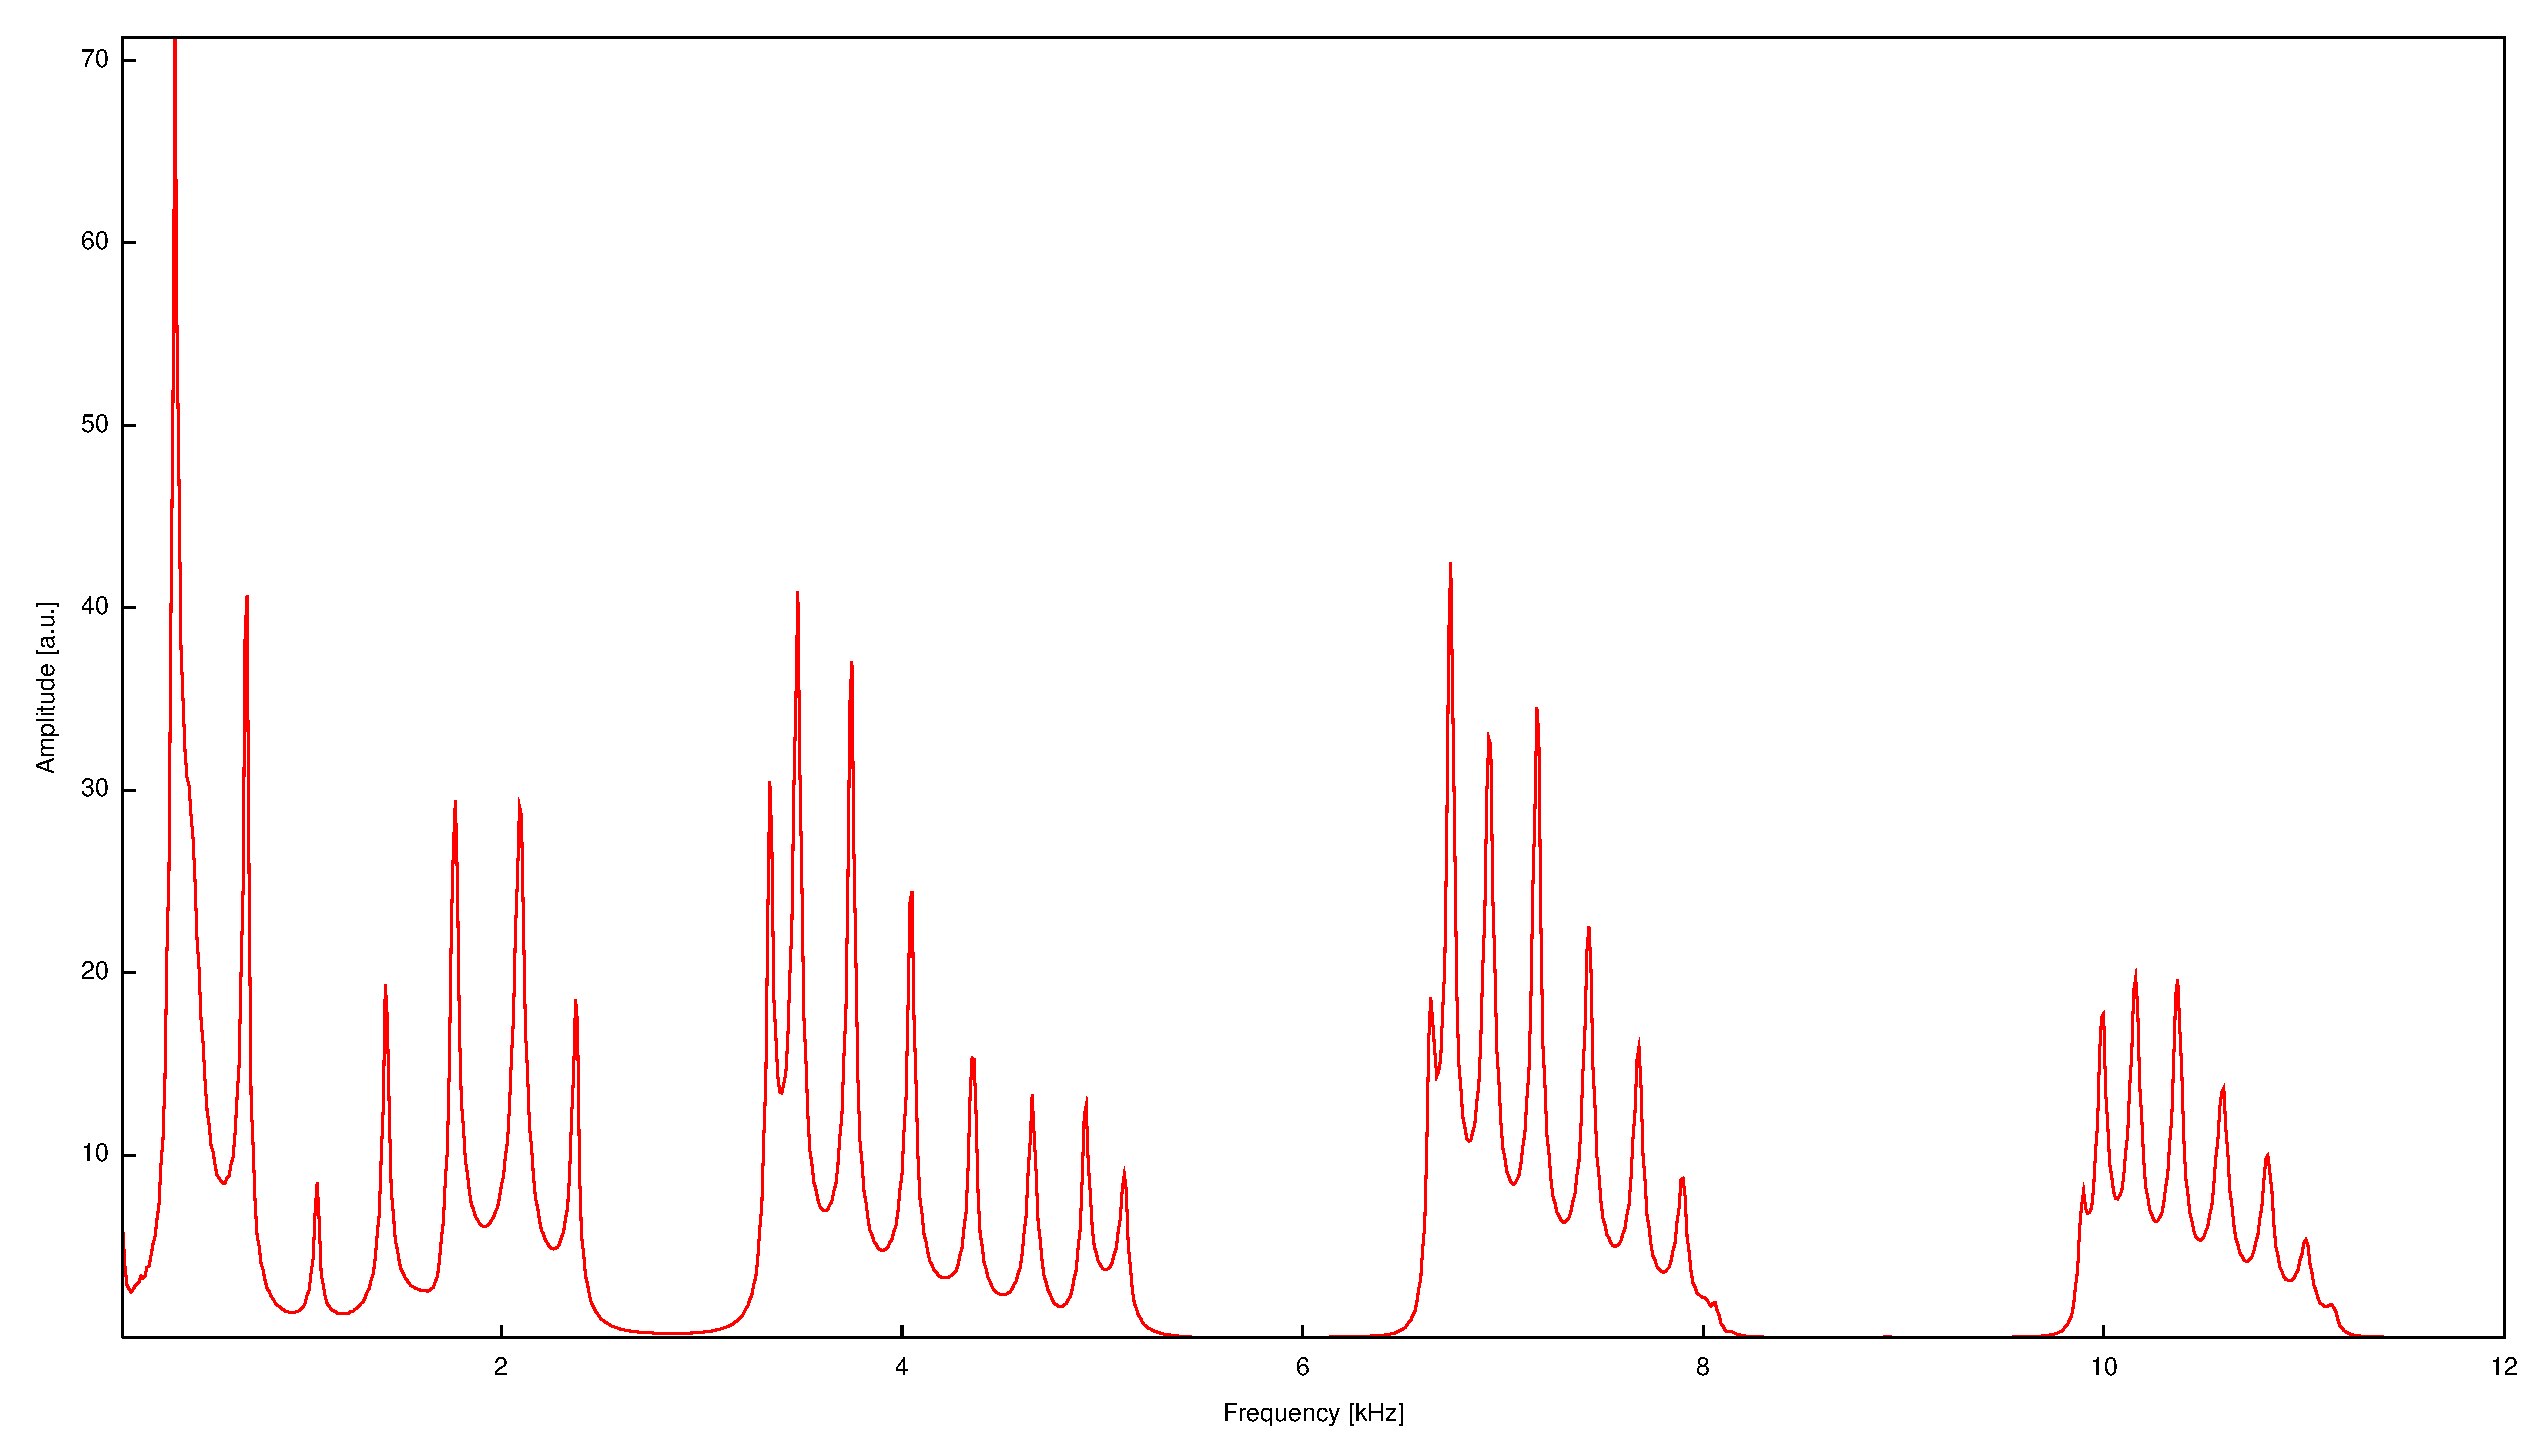
\includegraphics[width=\linewidth-60pt,height=\textheight-60pt,keepaspectratio]{FP-V23data/4.3_400mm_16mm.eps}
\caption{Spektrum von acht über $\SI{16}{\milli\meter}$-Iriden gekoppelten $\SI{50}{\milli\meter}$-Röhren.}
\label{fig:8_50_16}
\end{figure}

\begin{figure}
\centering
\includegraphics[width=\linewidth-60pt,height=\textheight-60pt,keepaspectratio]{build/4.3_10mm_reduced.pdf}
\caption{Dispersionsrelation im reduzierten Zonenschema bei acht über $\SI{10}{\milli\meter}$-Iriden gekoppelten $\SI{50}{\milli\meter}$-Röhren.}
\label{fig:w_k_1}
\end{figure}

\begin{figure}
\centering
\includegraphics[width=\linewidth-60pt,height=\textheight-60pt,keepaspectratio]{build/4.3_13mm_reduced.pdf}
\caption{Dispersionsrelation im reduzierten Zonenschema bei acht über $\SI{13}{\milli\meter}$-Iriden gekoppelten $\SI{50}{\milli\meter}$-Röhren.}
\label{fig:w_k_2}
\end{figure}

\begin{figure}
\centering
\includegraphics[width=\linewidth-60pt,height=\textheight-60pt,keepaspectratio]{build/4.3_16mm_reduced.pdf}
\caption{Dispersionsrelation im reduzierten Zonenschema bei acht über $\SI{16}{\milli\meter}$-Iriden gekoppelten $\SI{50}{\milli\meter}$-Röhren.}
\label{fig:w_k_3}
\end{figure}

\newpage
\noindent In den Abbildungen \ref{fig:10_50_16} und \ref{fig:12_50_16} sind die Spektren für zehn und zwölf über $\SI{16}{\milli\meter}$-Iriden gekoppelte $\SI{50}{\milli\meter}$-Röhren zu sehen. Im Vergleich zu \ref{fig:8_50_16} zeigt sich, dass während die Lage der Peaks  mit zunehmender Röhrenlänge nahezu unverändert ist, die Amplitude aller Peaks mit Ausnahme des zweiten abfallen, während dieser stark anwächst. Zudem ist die Anzahl der Peaks $P$ pro Band direkt abhängig von der Anzahl der Segmente $S$ der Röhre mit $P=S$.\\
In Abbildung \ref{fig:8_75_16} ist das Spektrum von acht über $\SI{16}{\milli\meter}$-Iriden gekoppelten $\SI{75}{\milli\meter}$-Röhren zu sehen. Der Vergleich mit Abbildung \ref{fig:8_50_16} zeigt, das bei längeren Teilstücken die Dichte der Bänder direkt proportional zur Länge der Teilstücke zunimmt.\\

\begin{figure}
\centering
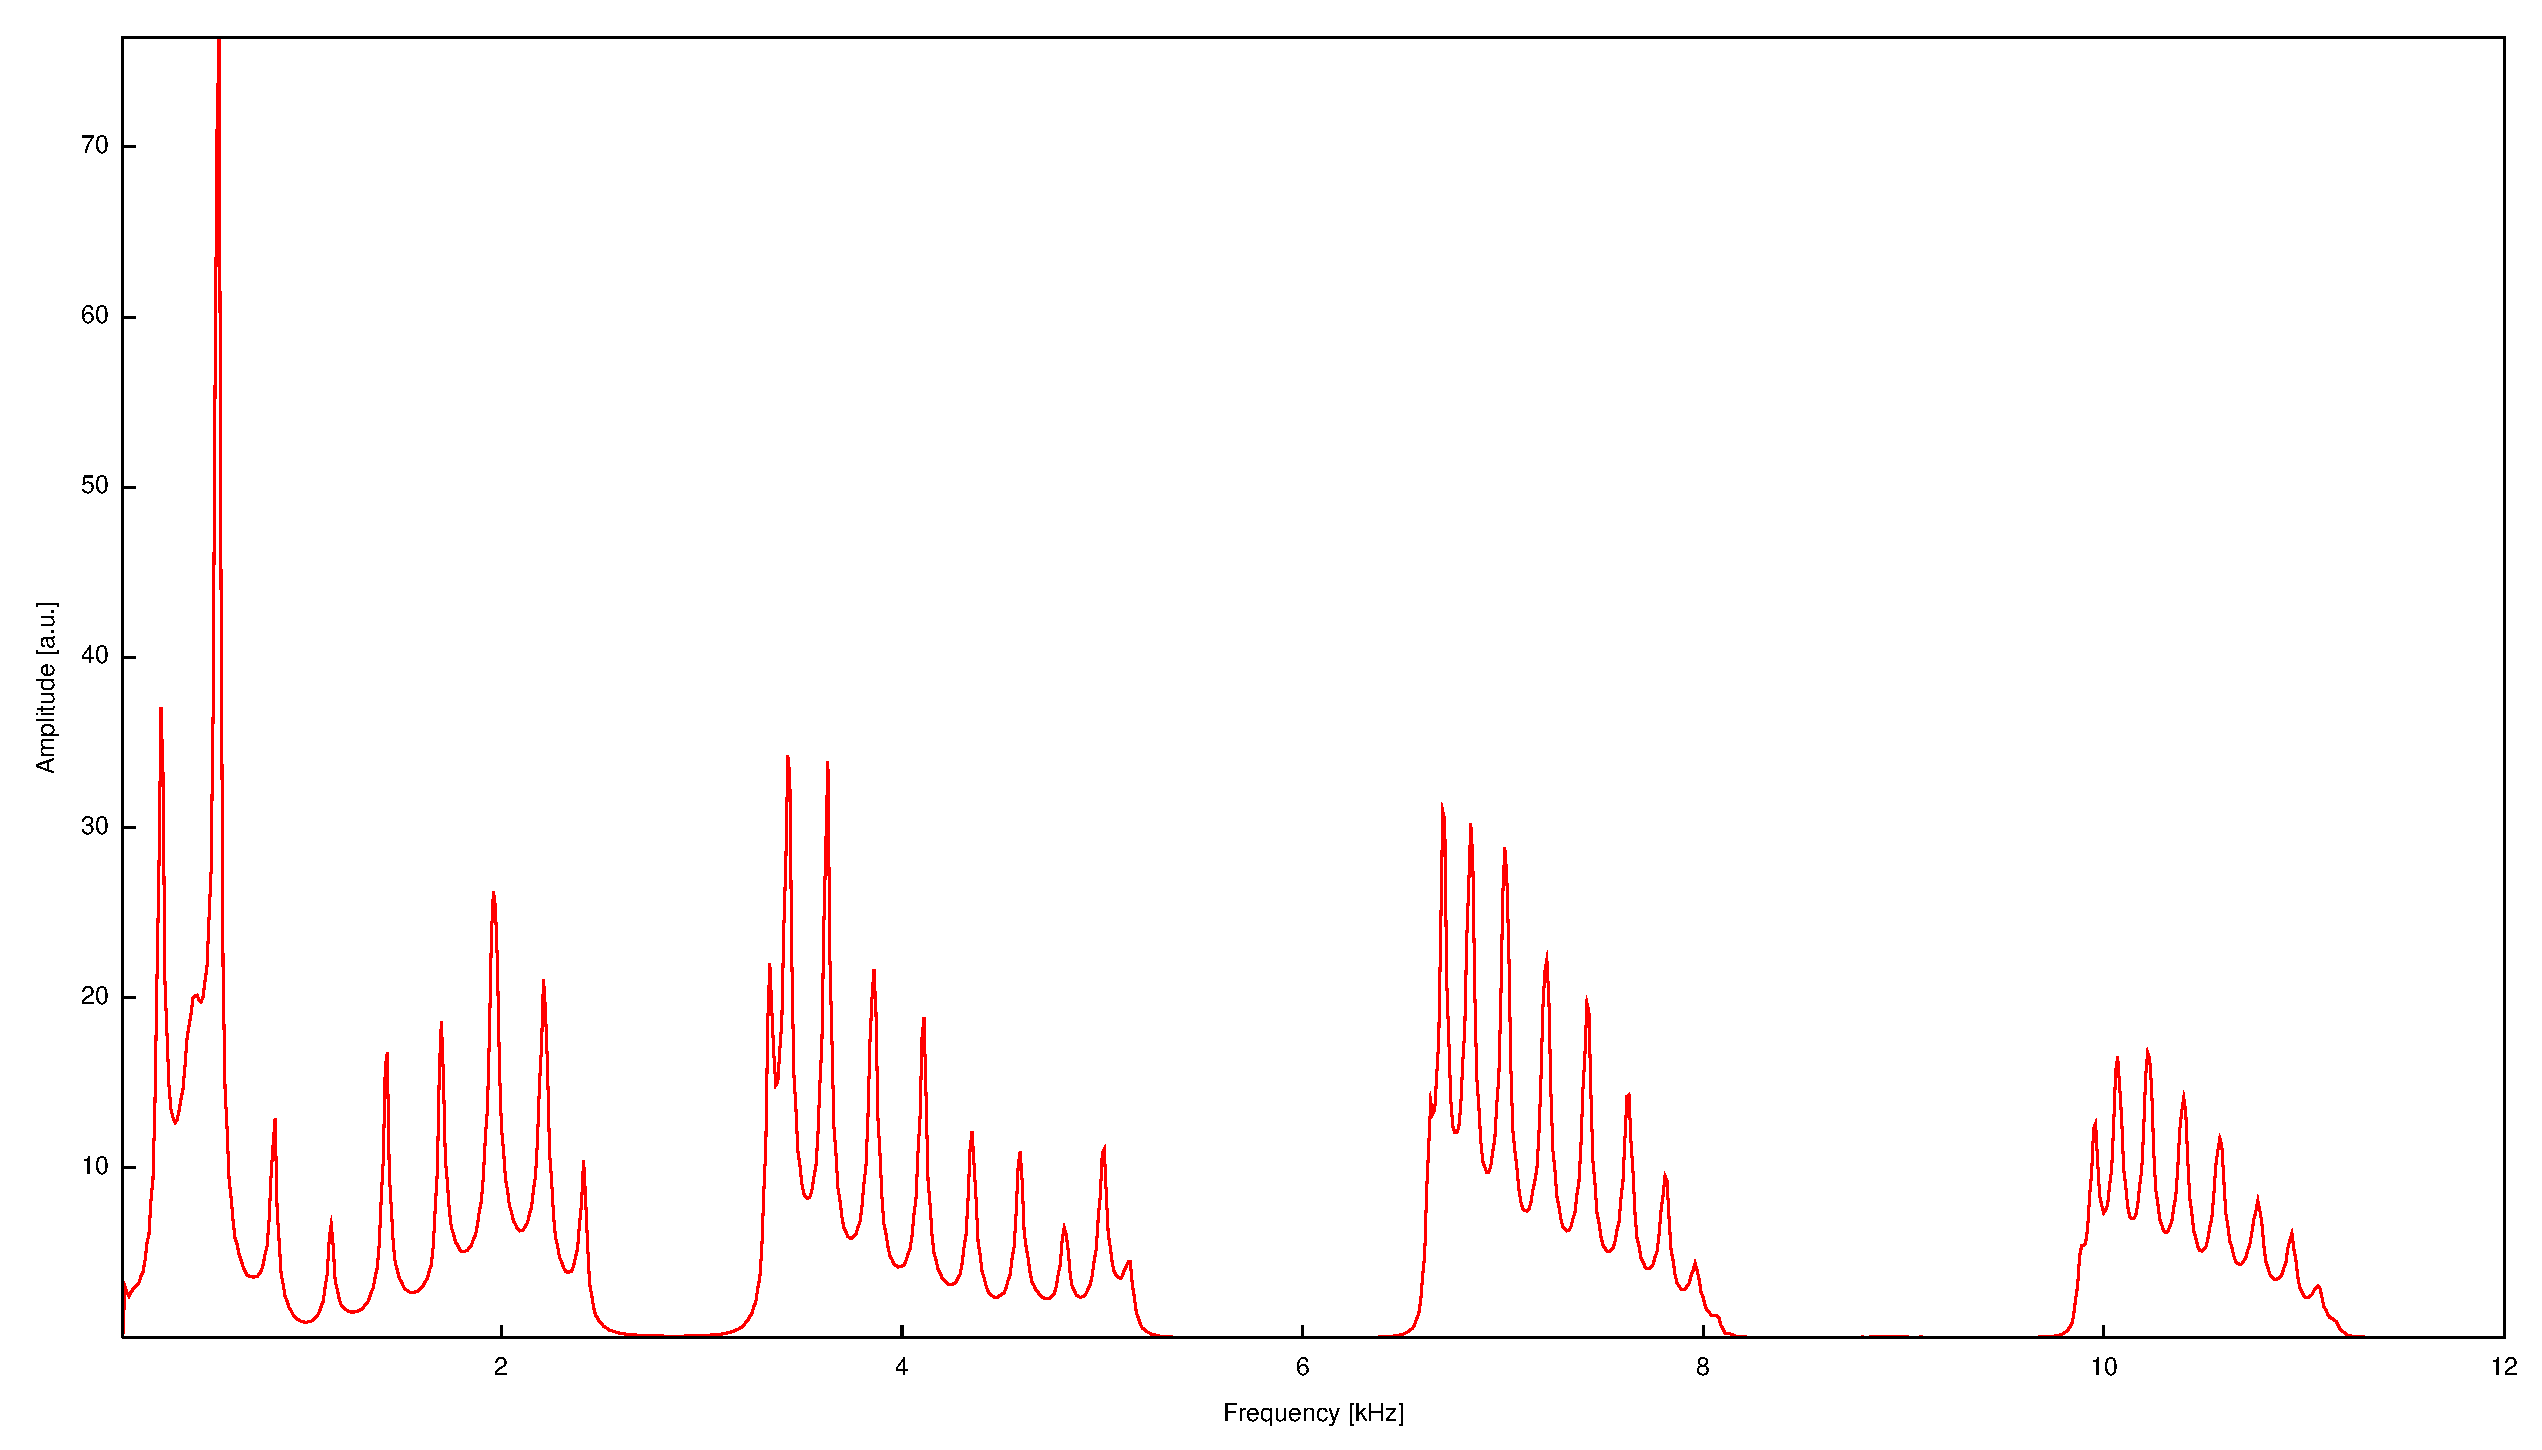
\includegraphics[width=\linewidth-60pt,height=\textheight-60pt,keepaspectratio]{FP-V23data/4.4_500mm_16mm.eps}
\caption{Spektrum von zehn über $\SI{16}{\milli\meter}$-Iriden gekoppelten $\SI{50}{\milli\meter}$-Röhren.}
\label{fig:10_50_16}
\end{figure}

\begin{figure}
\centering
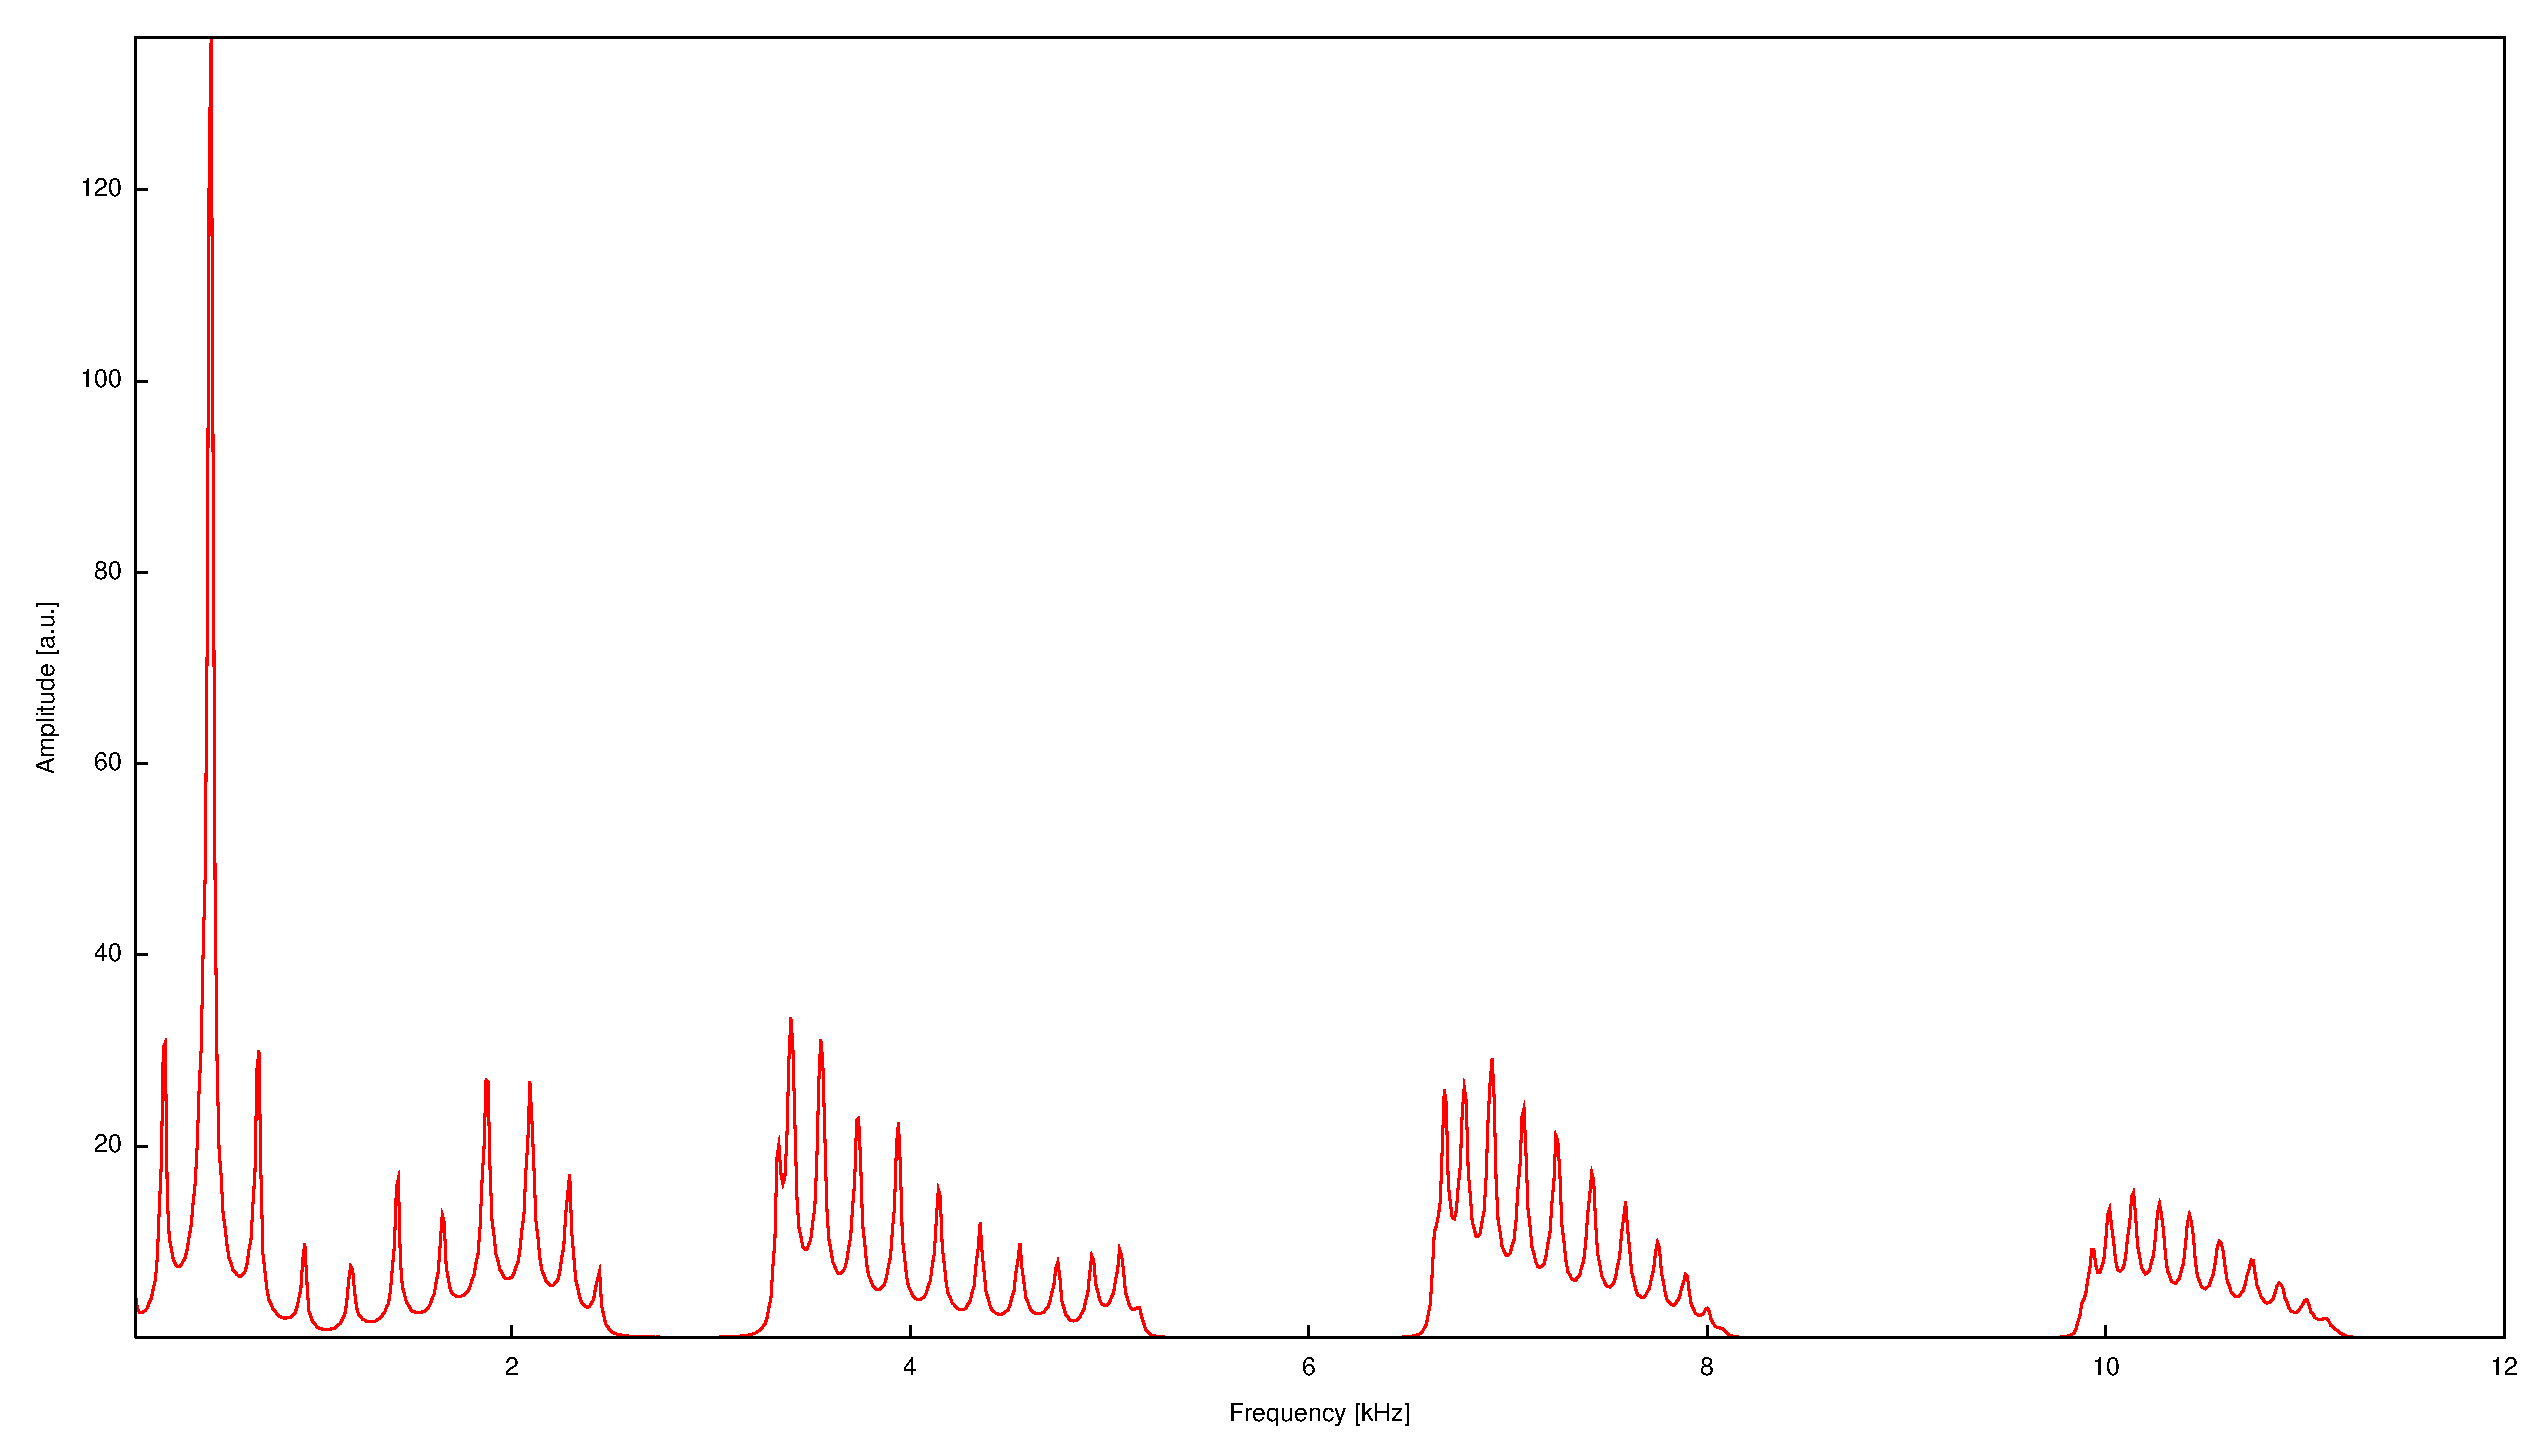
\includegraphics[width=\linewidth-60pt,height=\textheight-60pt,keepaspectratio]{FP-V23data/4.4_600mm_16mm.eps}
\caption{Spektrum von zwölf über $\SI{16}{\milli\meter}$-Iriden gekoppelten $\SI{50}{\milli\meter}$-Röhren.}
\label{fig:12_50_16}
\end{figure}

\begin{figure}
\centering
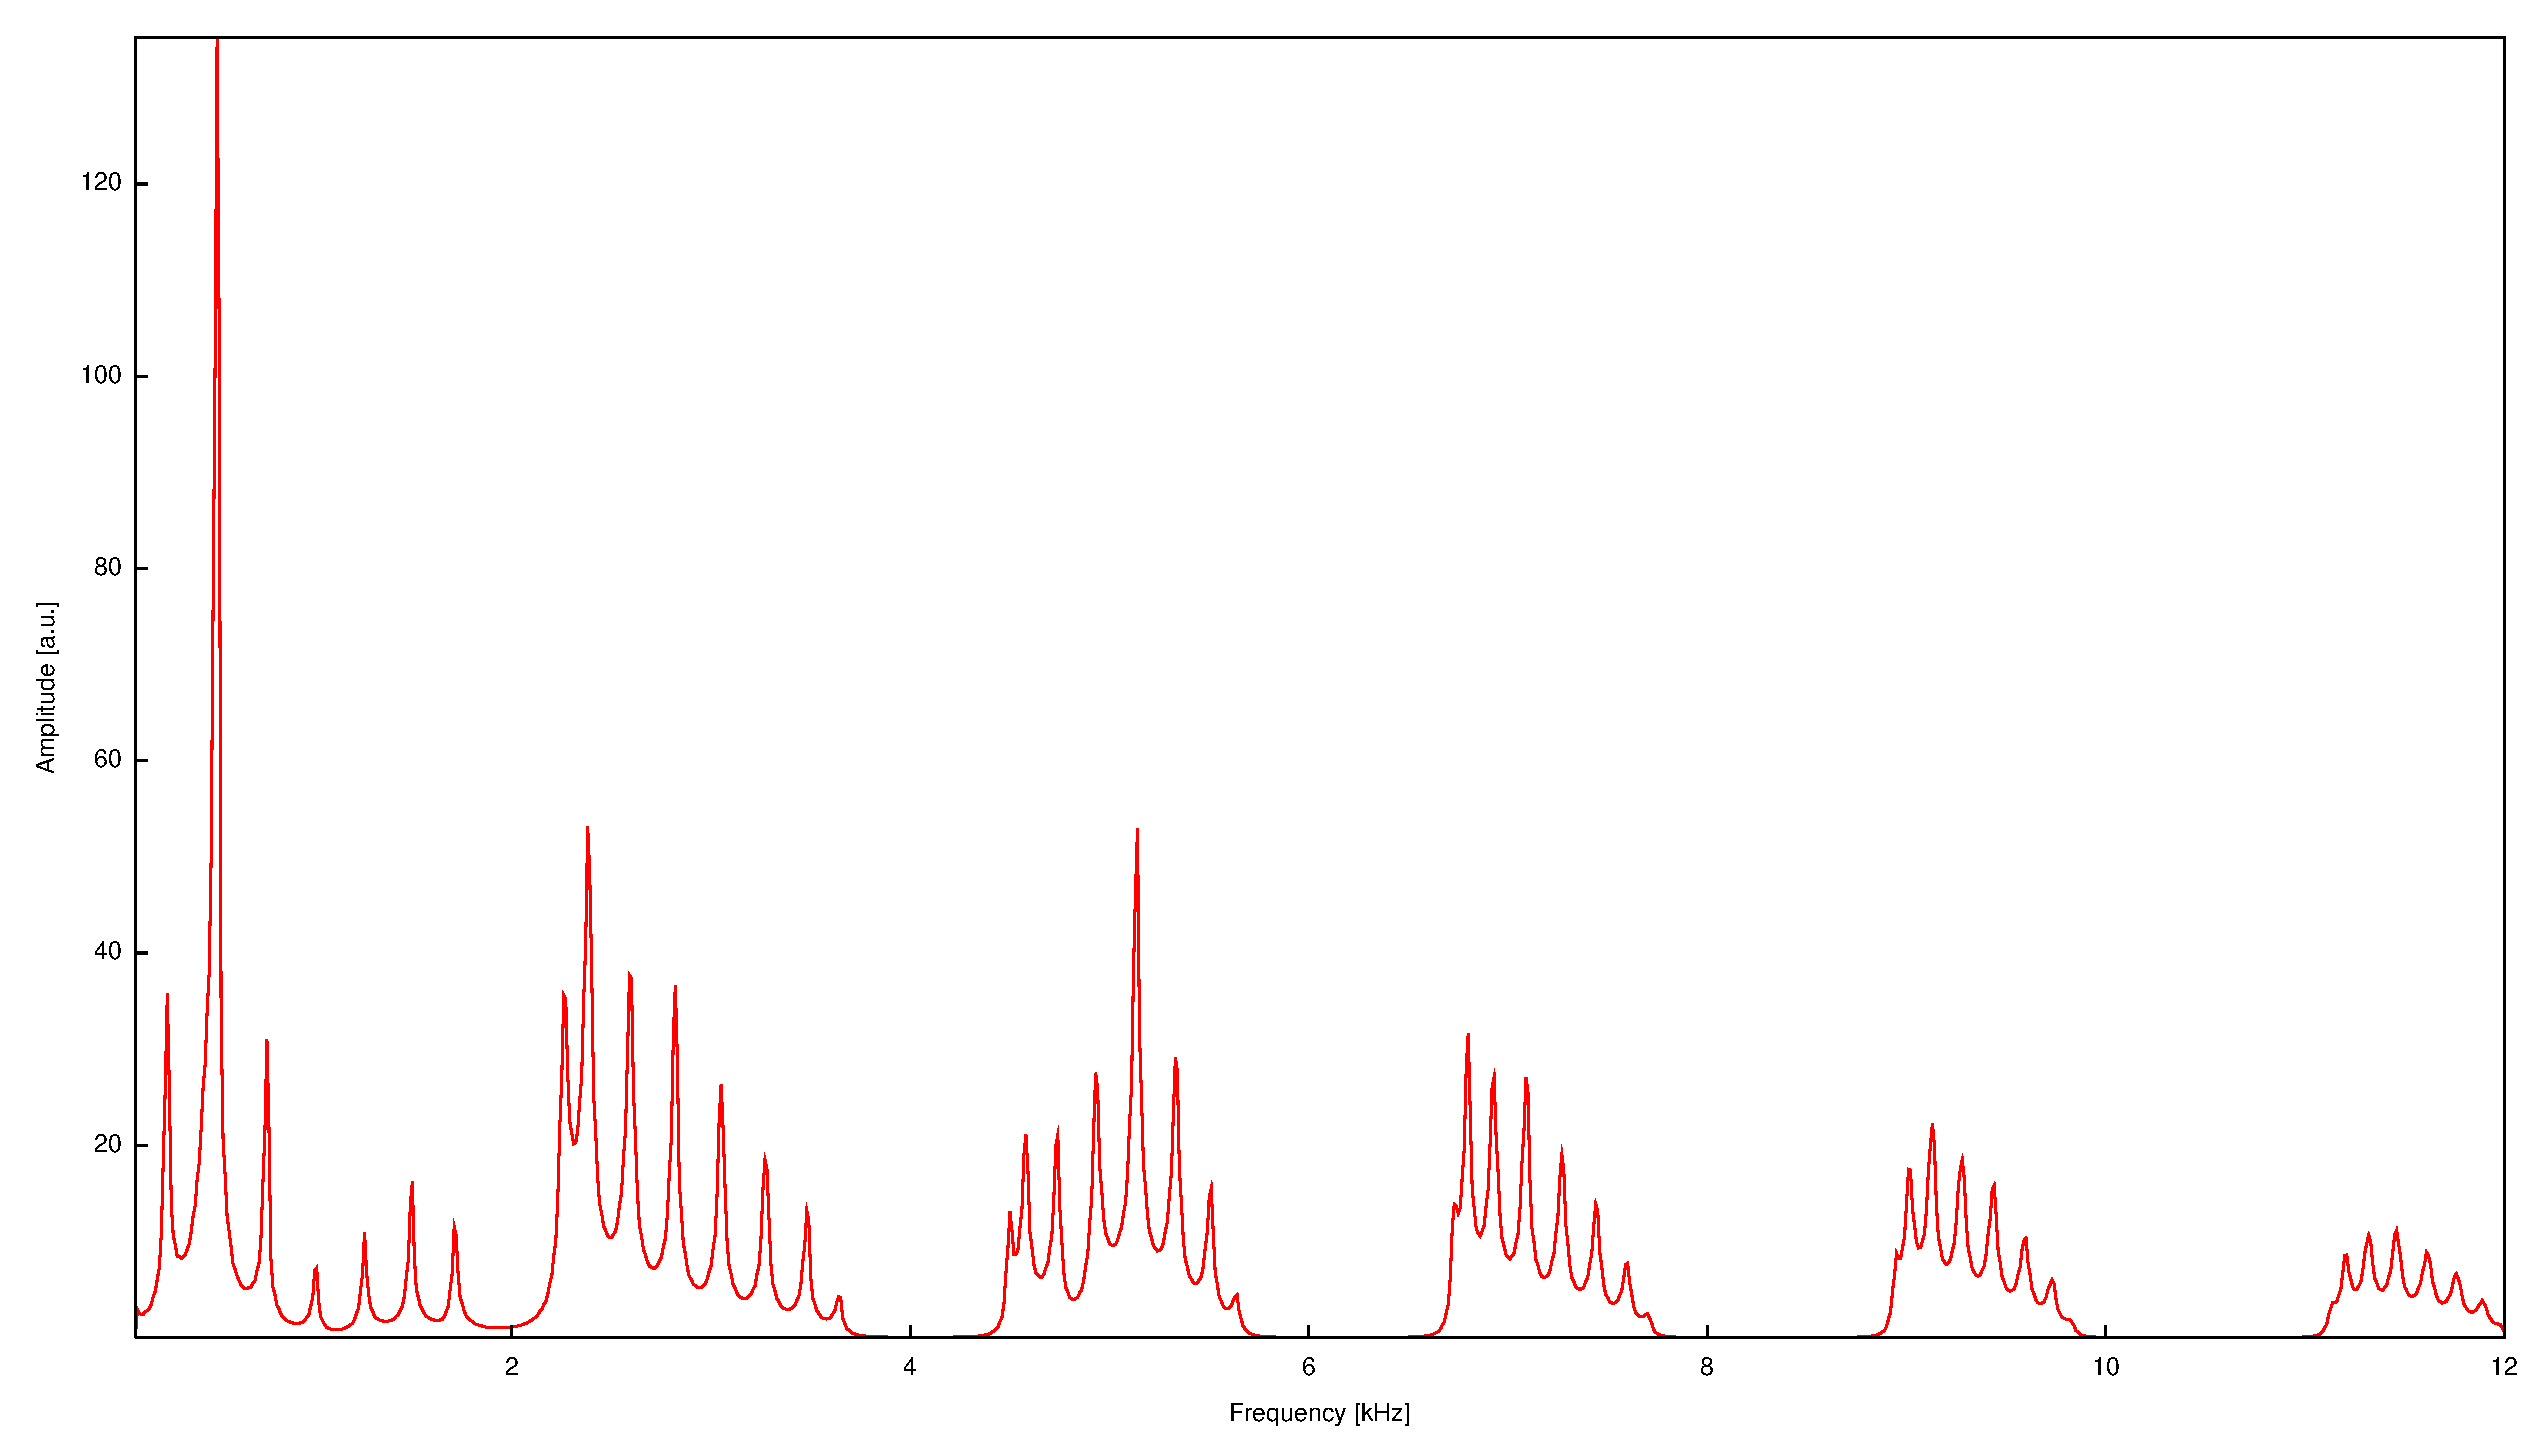
\includegraphics[width=\linewidth-60pt,height=\textheight-60pt,keepaspectratio]{FP-V23data/4.5_600mm_16mm.eps}
\caption{Spektrum von acht über $\SI{16}{\milli\meter}$-Iriden gekoppelten $\SI{75}{\milli\meter}$-Röhren.}
\label{fig:8_75_16}
\end{figure}

\newpage
\noindent Mit den Daten aus Abbildung \ref{fig:8_50_16} kann mit
\[
\rho(f) = \frac{1}{f_{n+1}-f_n}
\]
die Zustandsdichte ermittelt werden. Sie ist in Abbildung \ref{fig:DOS} gegen die Frequenz aufgetragen. Es ist zu erkennen, dass die Zustandsdichte an den Rändern der Bänder zunimmt.

\begin{figure}
\centering
\includegraphics[width=\linewidth-60pt,height=\textheight-60pt,keepaspectratio]{build/4._DOS.pdf}
\caption{Die Zustandsdichte aufgetragen gegen die Frequenz.}
\label{fig:DOS}
\end{figure}

\subsubsection{Atom-Molekül-Kette und Fehlstellen}

In Abbildung \ref{fig:50mm} ist das Spektrum einer $\SI{50}{\milli\meter}$-Röhre von $\SI{100}{\hertz}$ bis $\SI{22000}{\hertz}$ zu sehen. Bis $f\approx\SI{15000}{\hertz}$
sind die Peaks äquidistante longitudinale Moden mit $\Delta f=\SI{3390(15)}{\hertz}$. Für höhere Frequenzen sind die Abstände nicht mehr gleichmäßig und die Amplituden der Peaks wesentlich geringer. Sie beschreiben die transversalen Moden der Schallwelle in der Röhre.\\
In Abbildung \ref{fig:75mm} ist dasselbe Spektrum für eine $\SI{75}{\milli\meter}$-Röhre aufgenommen. Auch hier sind die longitudinalen Moden durch äquidistante Peaks bis etwa $\SI{15000}{\hertz}$ zu erkennen mit $\Delta f=\SI{2268(6)}{\hertz}$.\\
In Abbildung \ref{fig:50_10_50} ist das Spektrum von $\SI{100}{\hertz}$ bis $\SI{22000}{\hertz}$ einer Einheitszelle bestehend aus zwei über eine $\SI{10}{\milli\meter}$-Iris gekoppelten $\SI{50}{\milli\meter}$-Röhren zu sehen. Dieselbe Messung für eine $\SI{16}{\milli\meter}$-Kopplung ist in Abbildung \ref{fig:50_16_50} zu sehen. Es zeigt sich, dass die Breite der Bänder bei größerer Kopplung steigt während die Höhe der Peaks abnimmt. Auch ist bei größerem Innendurchmesser der Iris ein stärkerer Untergrund zu beobachten.
Bei zunehmender Anzahl von Zellen ist eine stärkere Ausprägung der Bänder und Bandlücken zu beobachten.
%4.9 part2?

\begin{figure}
\centering
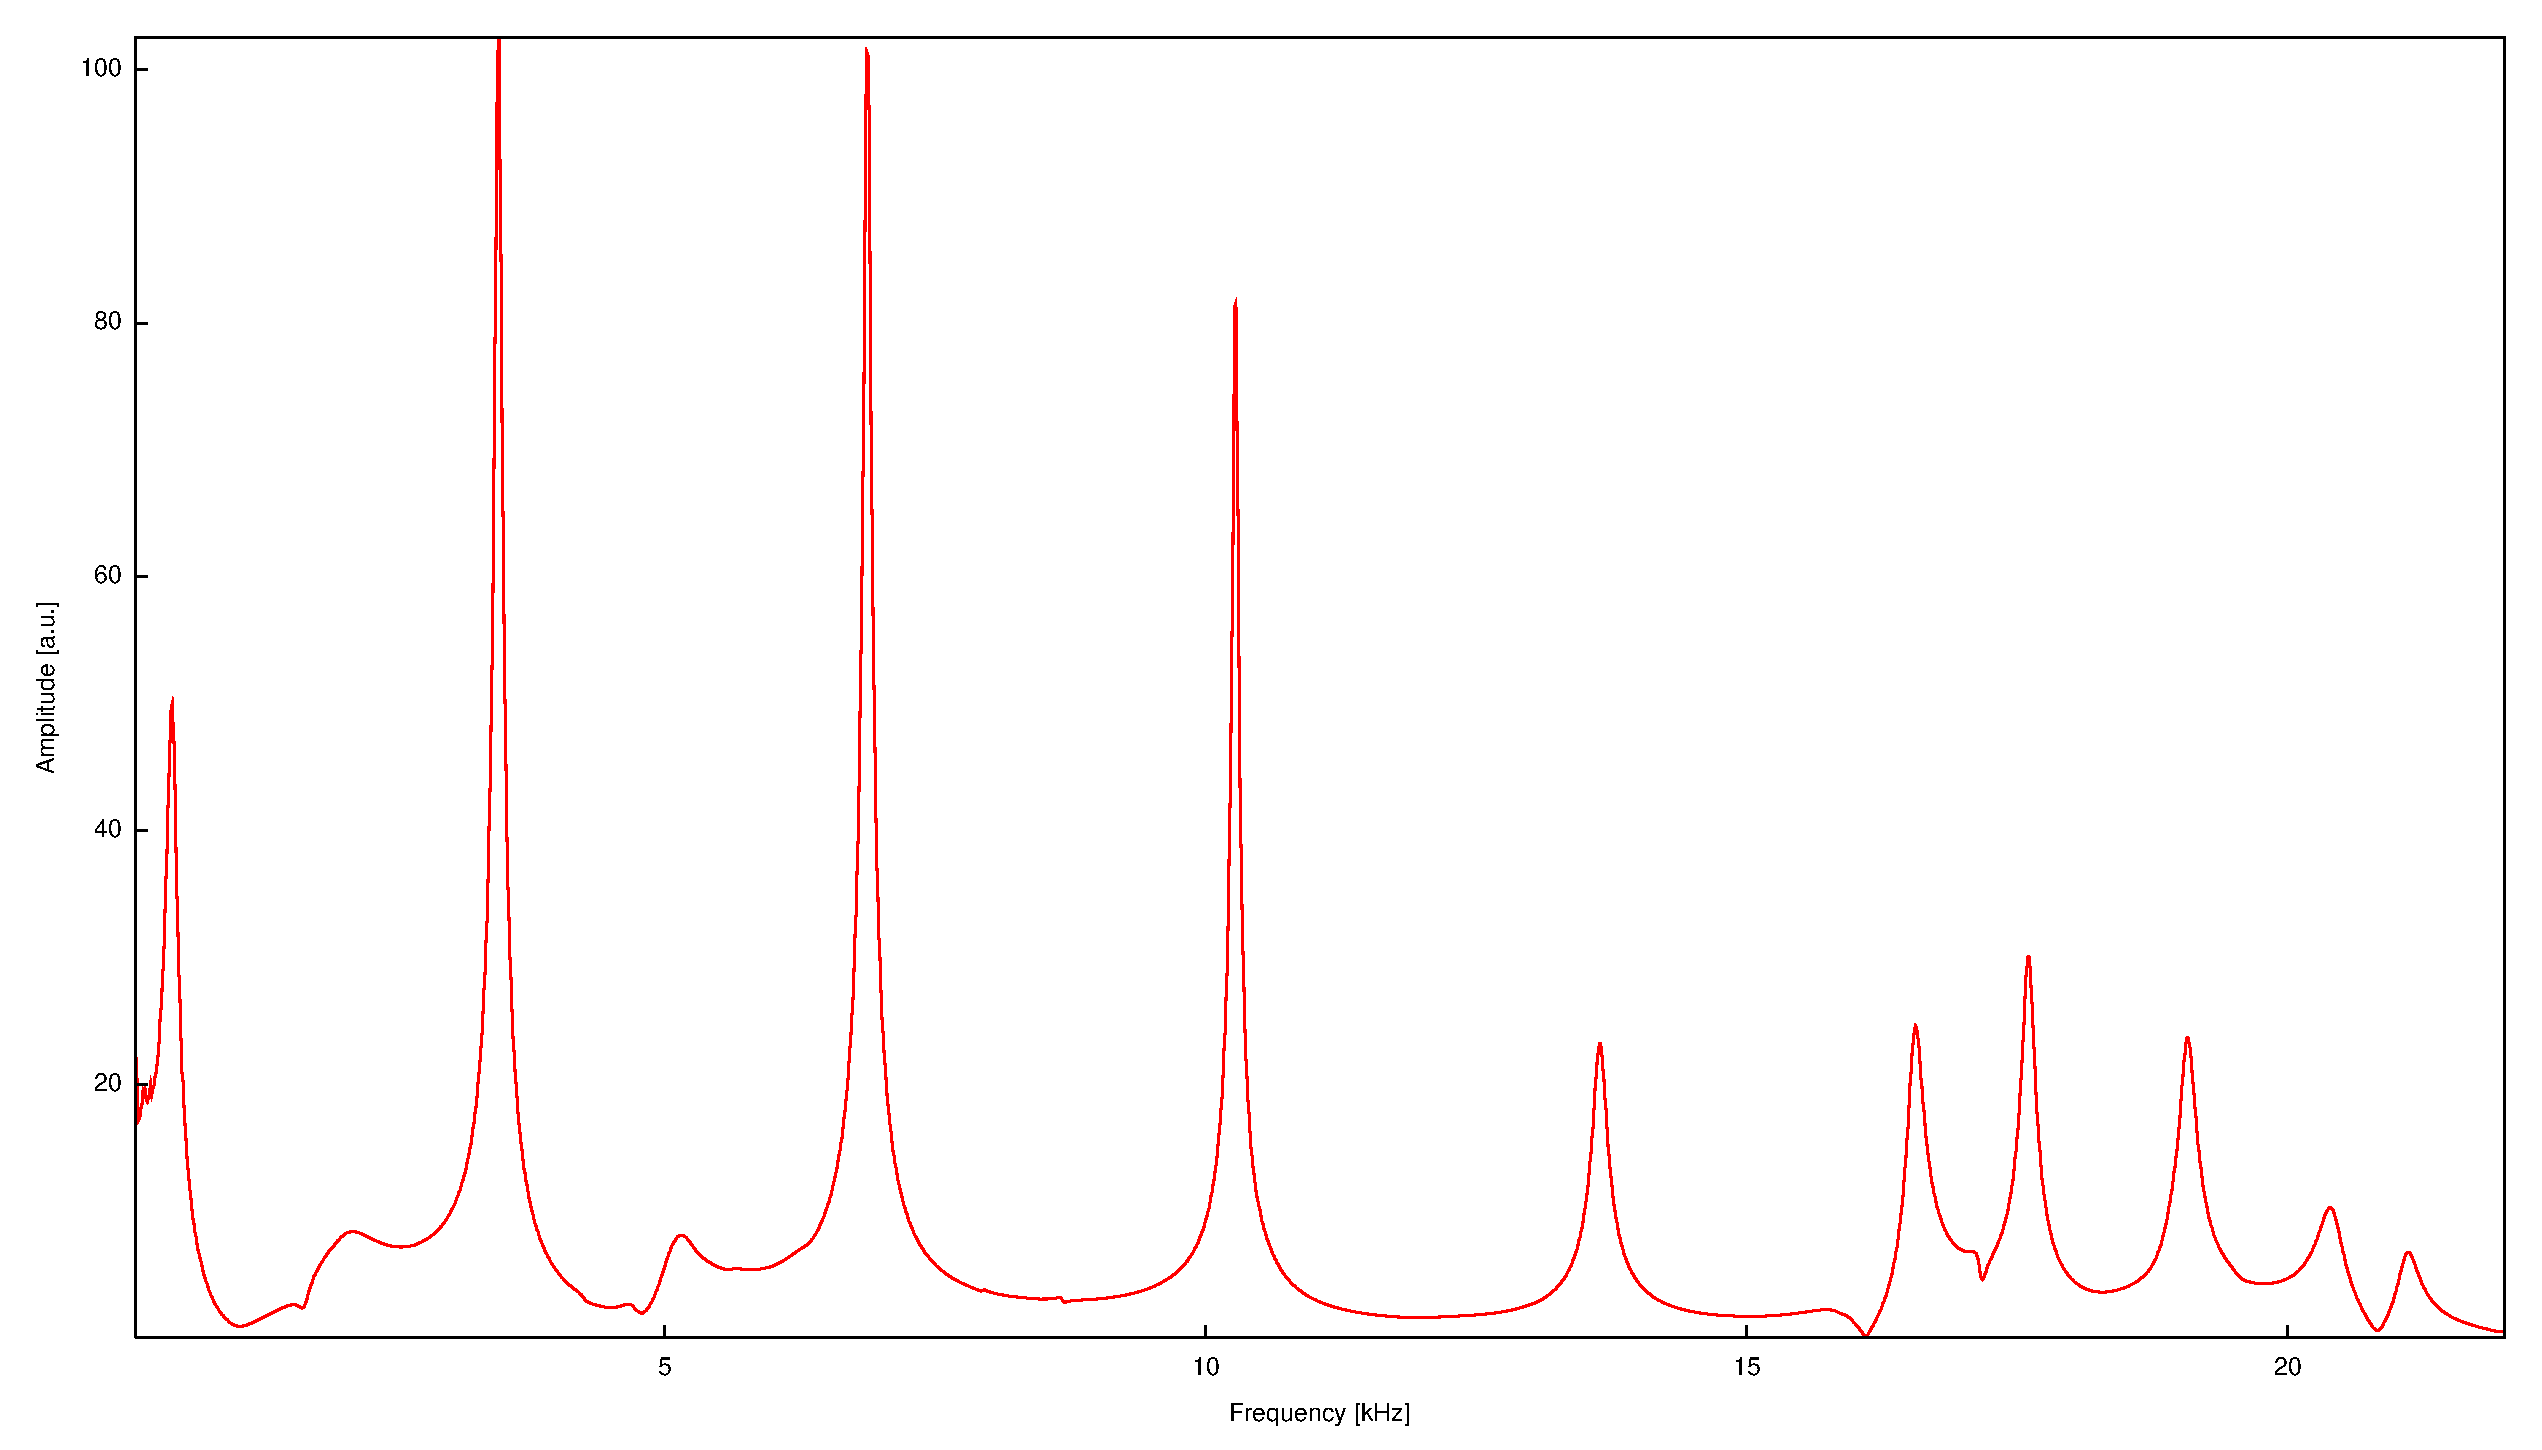
\includegraphics[width=\linewidth-60pt,height=\textheight-60pt,keepaspectratio]{FP-V23data/4.6_50mm.eps}
\caption{Spektrum von einer $\SI{50}{\milli\meter}$-Röhre.}
\label{fig:50mm}
\end{figure}

\begin{figure}
\centering
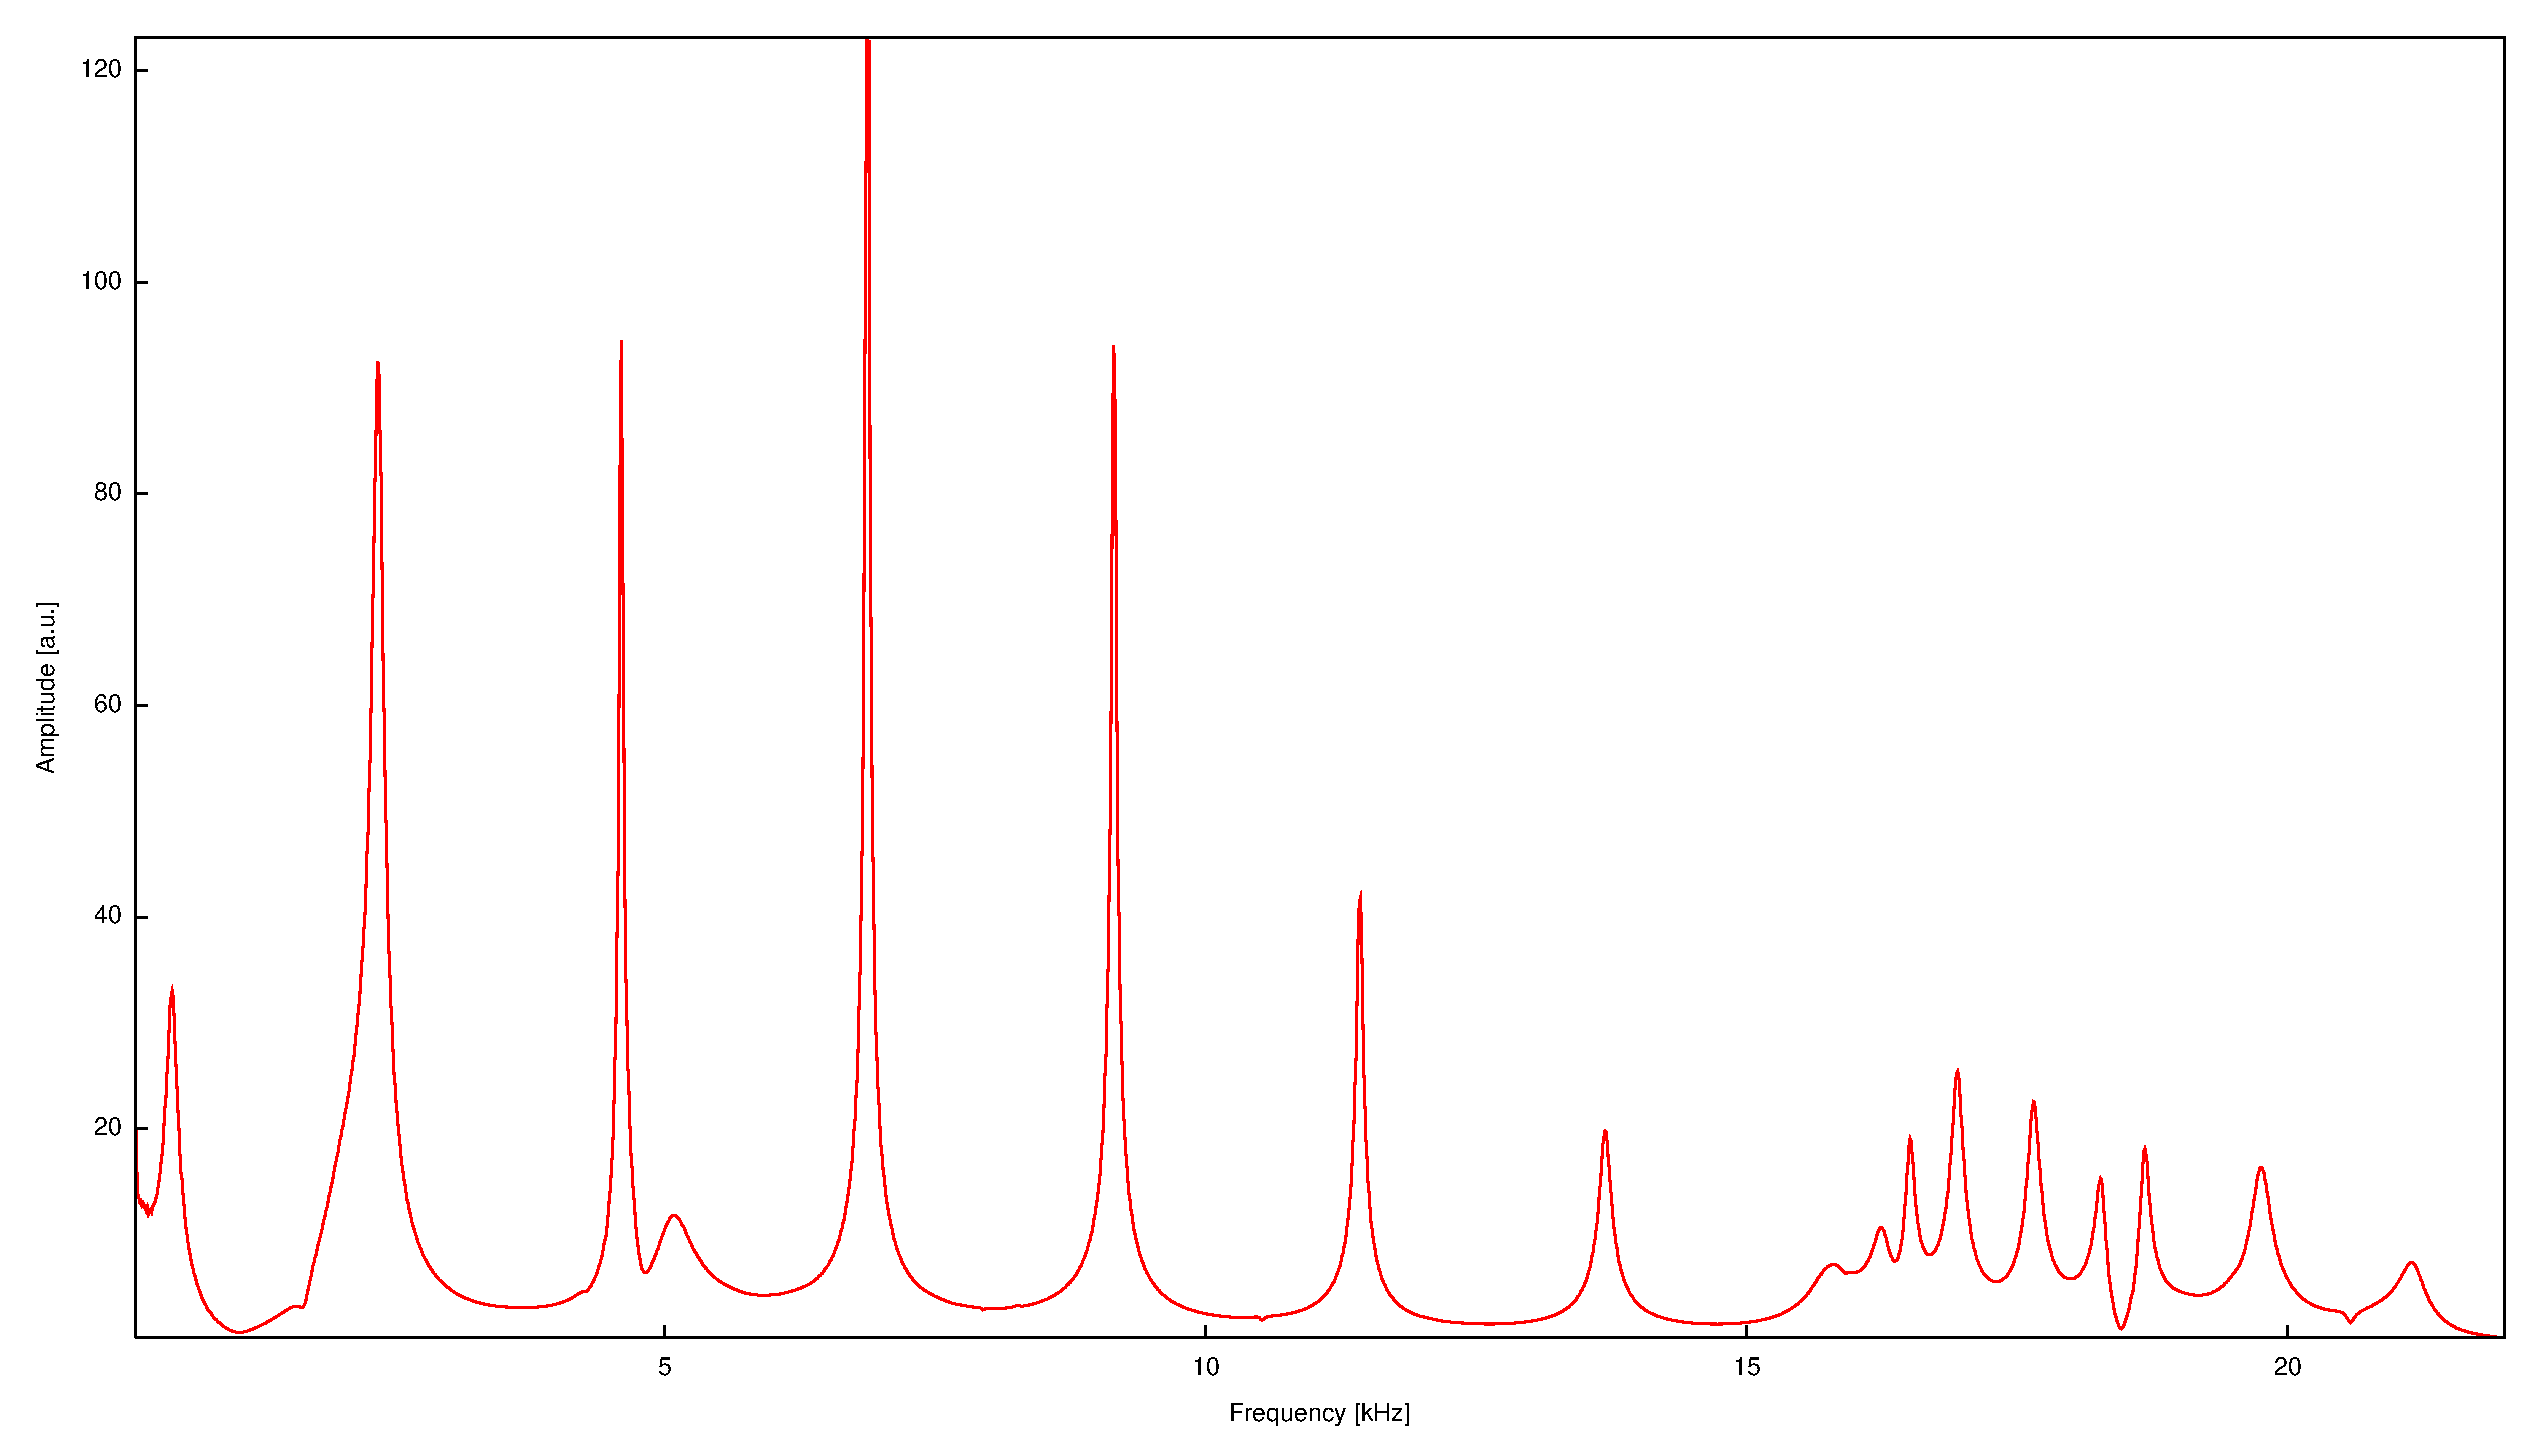
\includegraphics[width=\linewidth-60pt,height=\textheight-60pt,keepaspectratio]{FP-V23data/4.7_75mm.eps}
\caption{Spektrum von einer $\SI{75}{\milli\meter}$-Röhre.}
\label{fig:75mm}
\end{figure}

\begin{figure}
\centering
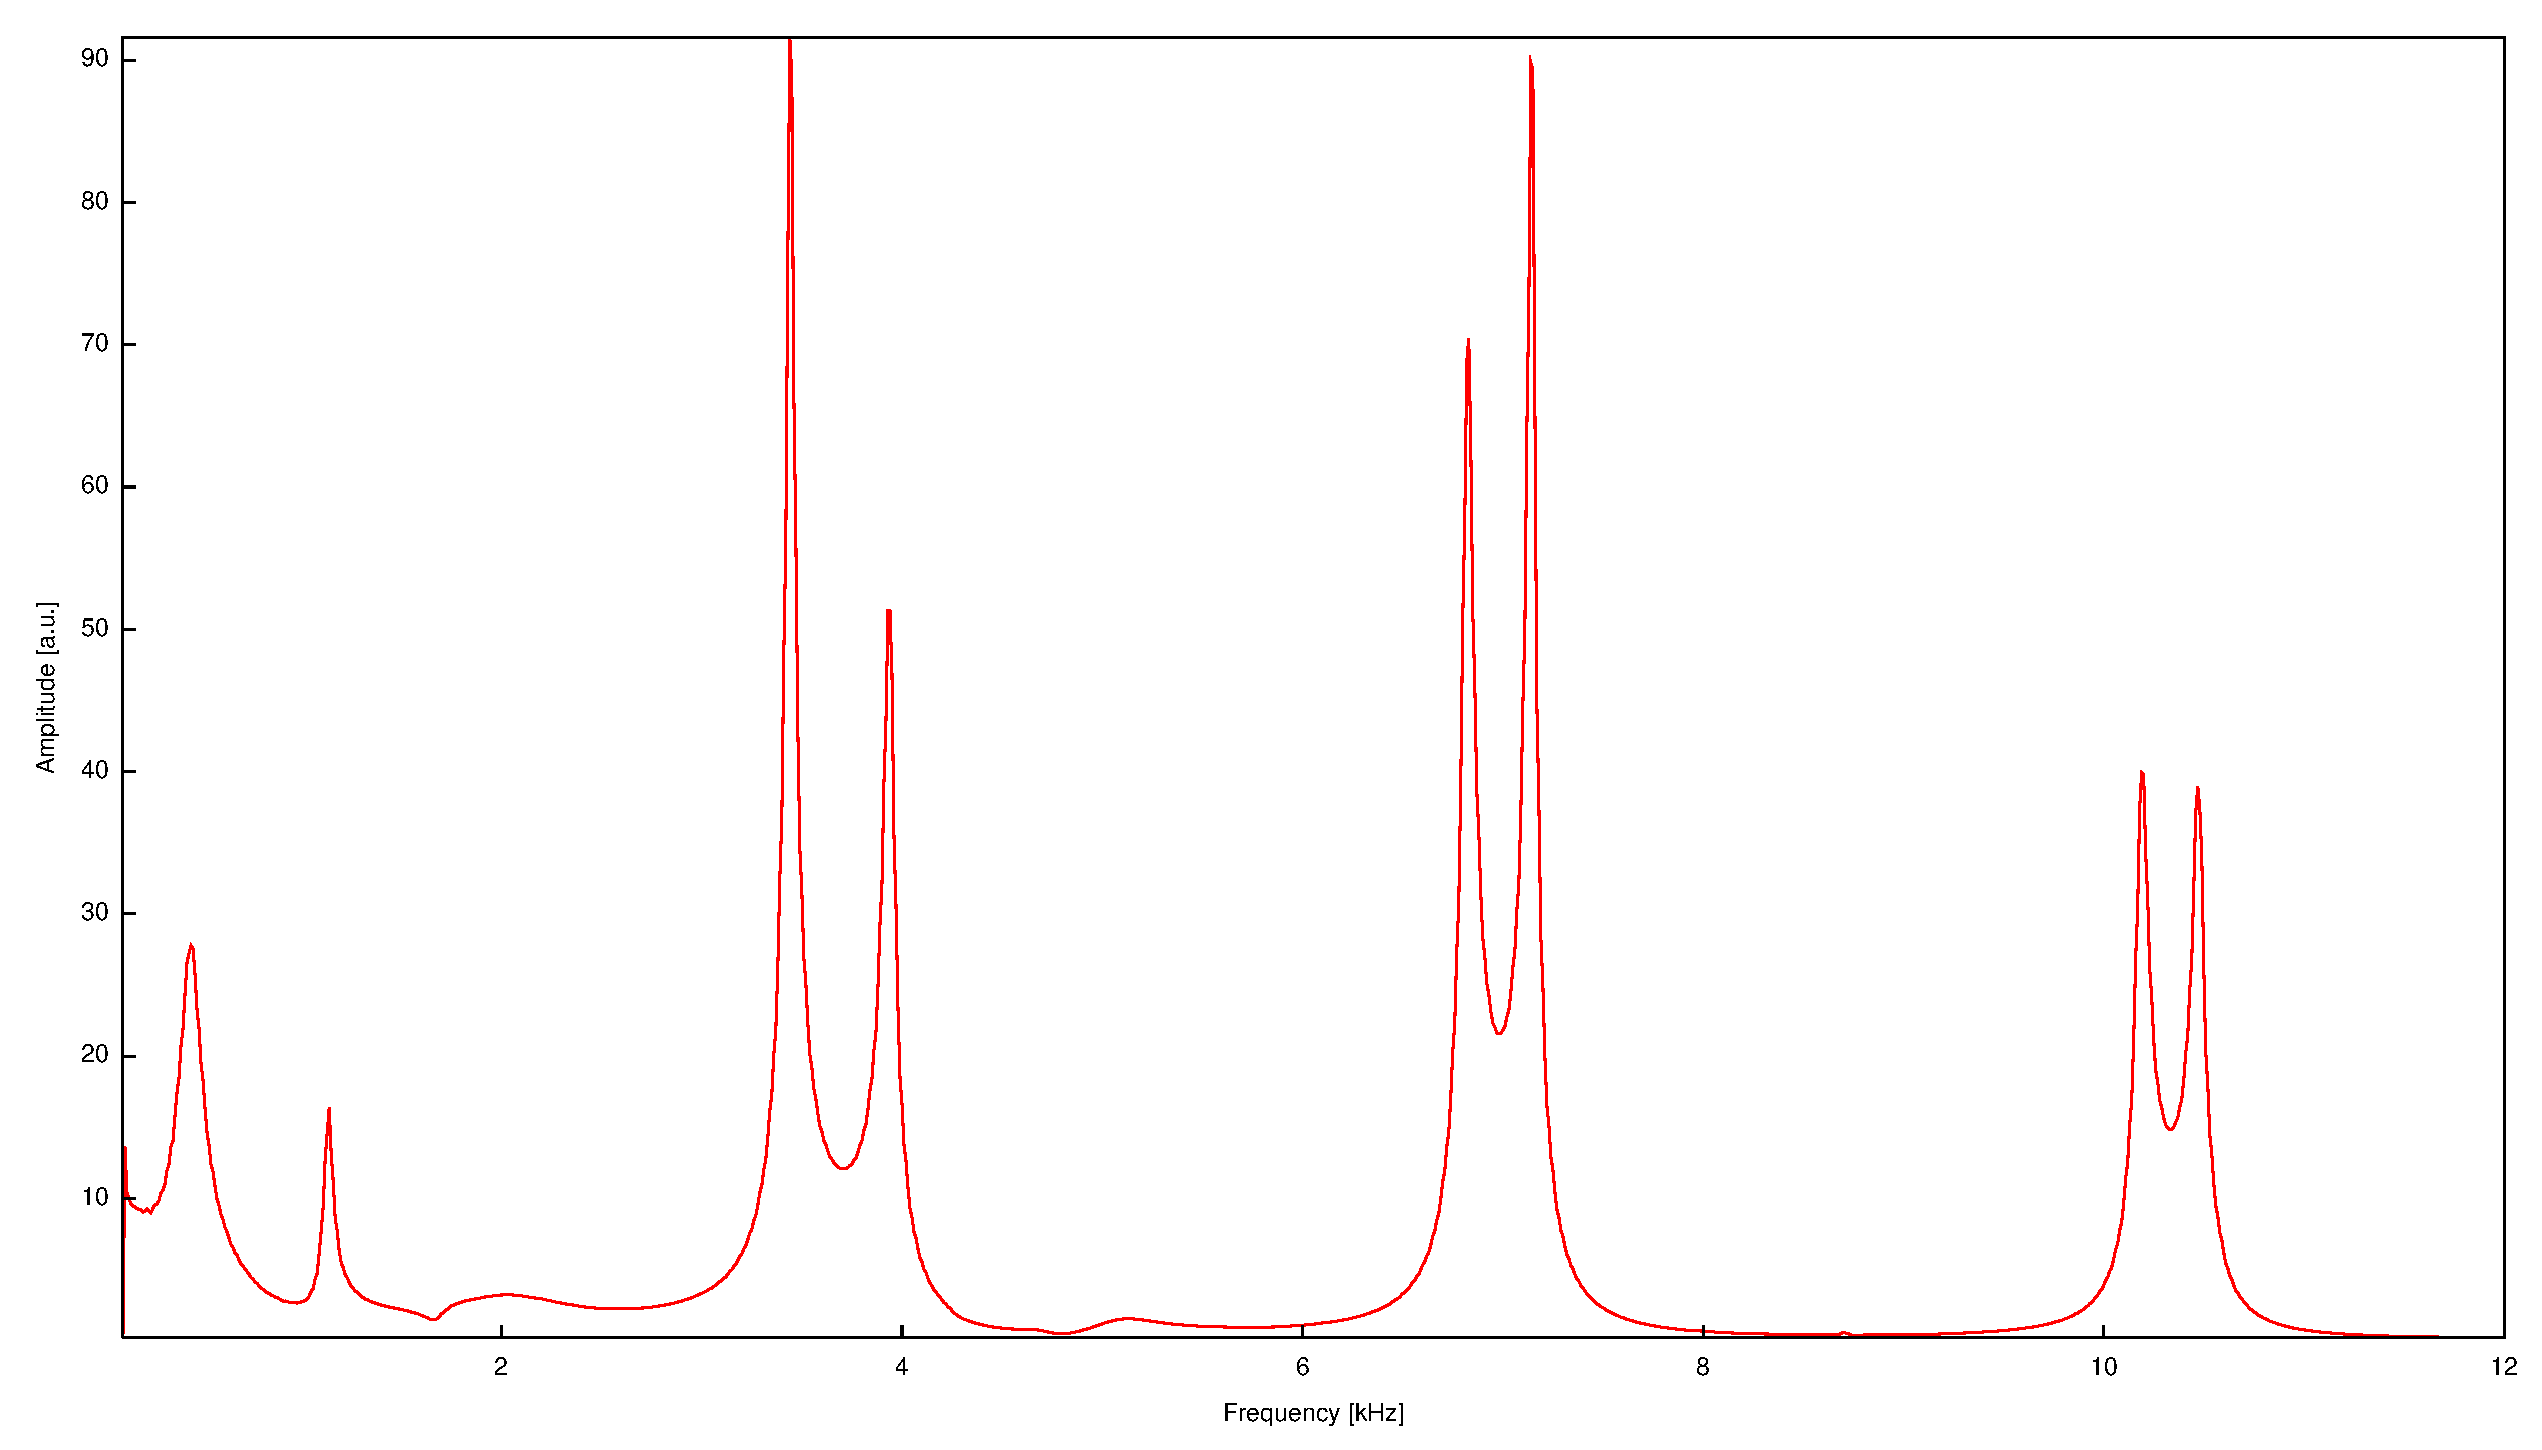
\includegraphics[width=\linewidth-60pt,height=\textheight-60pt,keepaspectratio]{FP-V23data/4.8_100mm_10mm.eps}
\caption{Spektrum von einer Einheitszelle bestehend aus zwei über $\SI{10}{\milli\meter}$-Iriden gekoppelten $\SI{50}{\milli\meter}$-Röhren.}
\label{fig:50_10_50}
\end{figure}

\begin{figure}
\centering
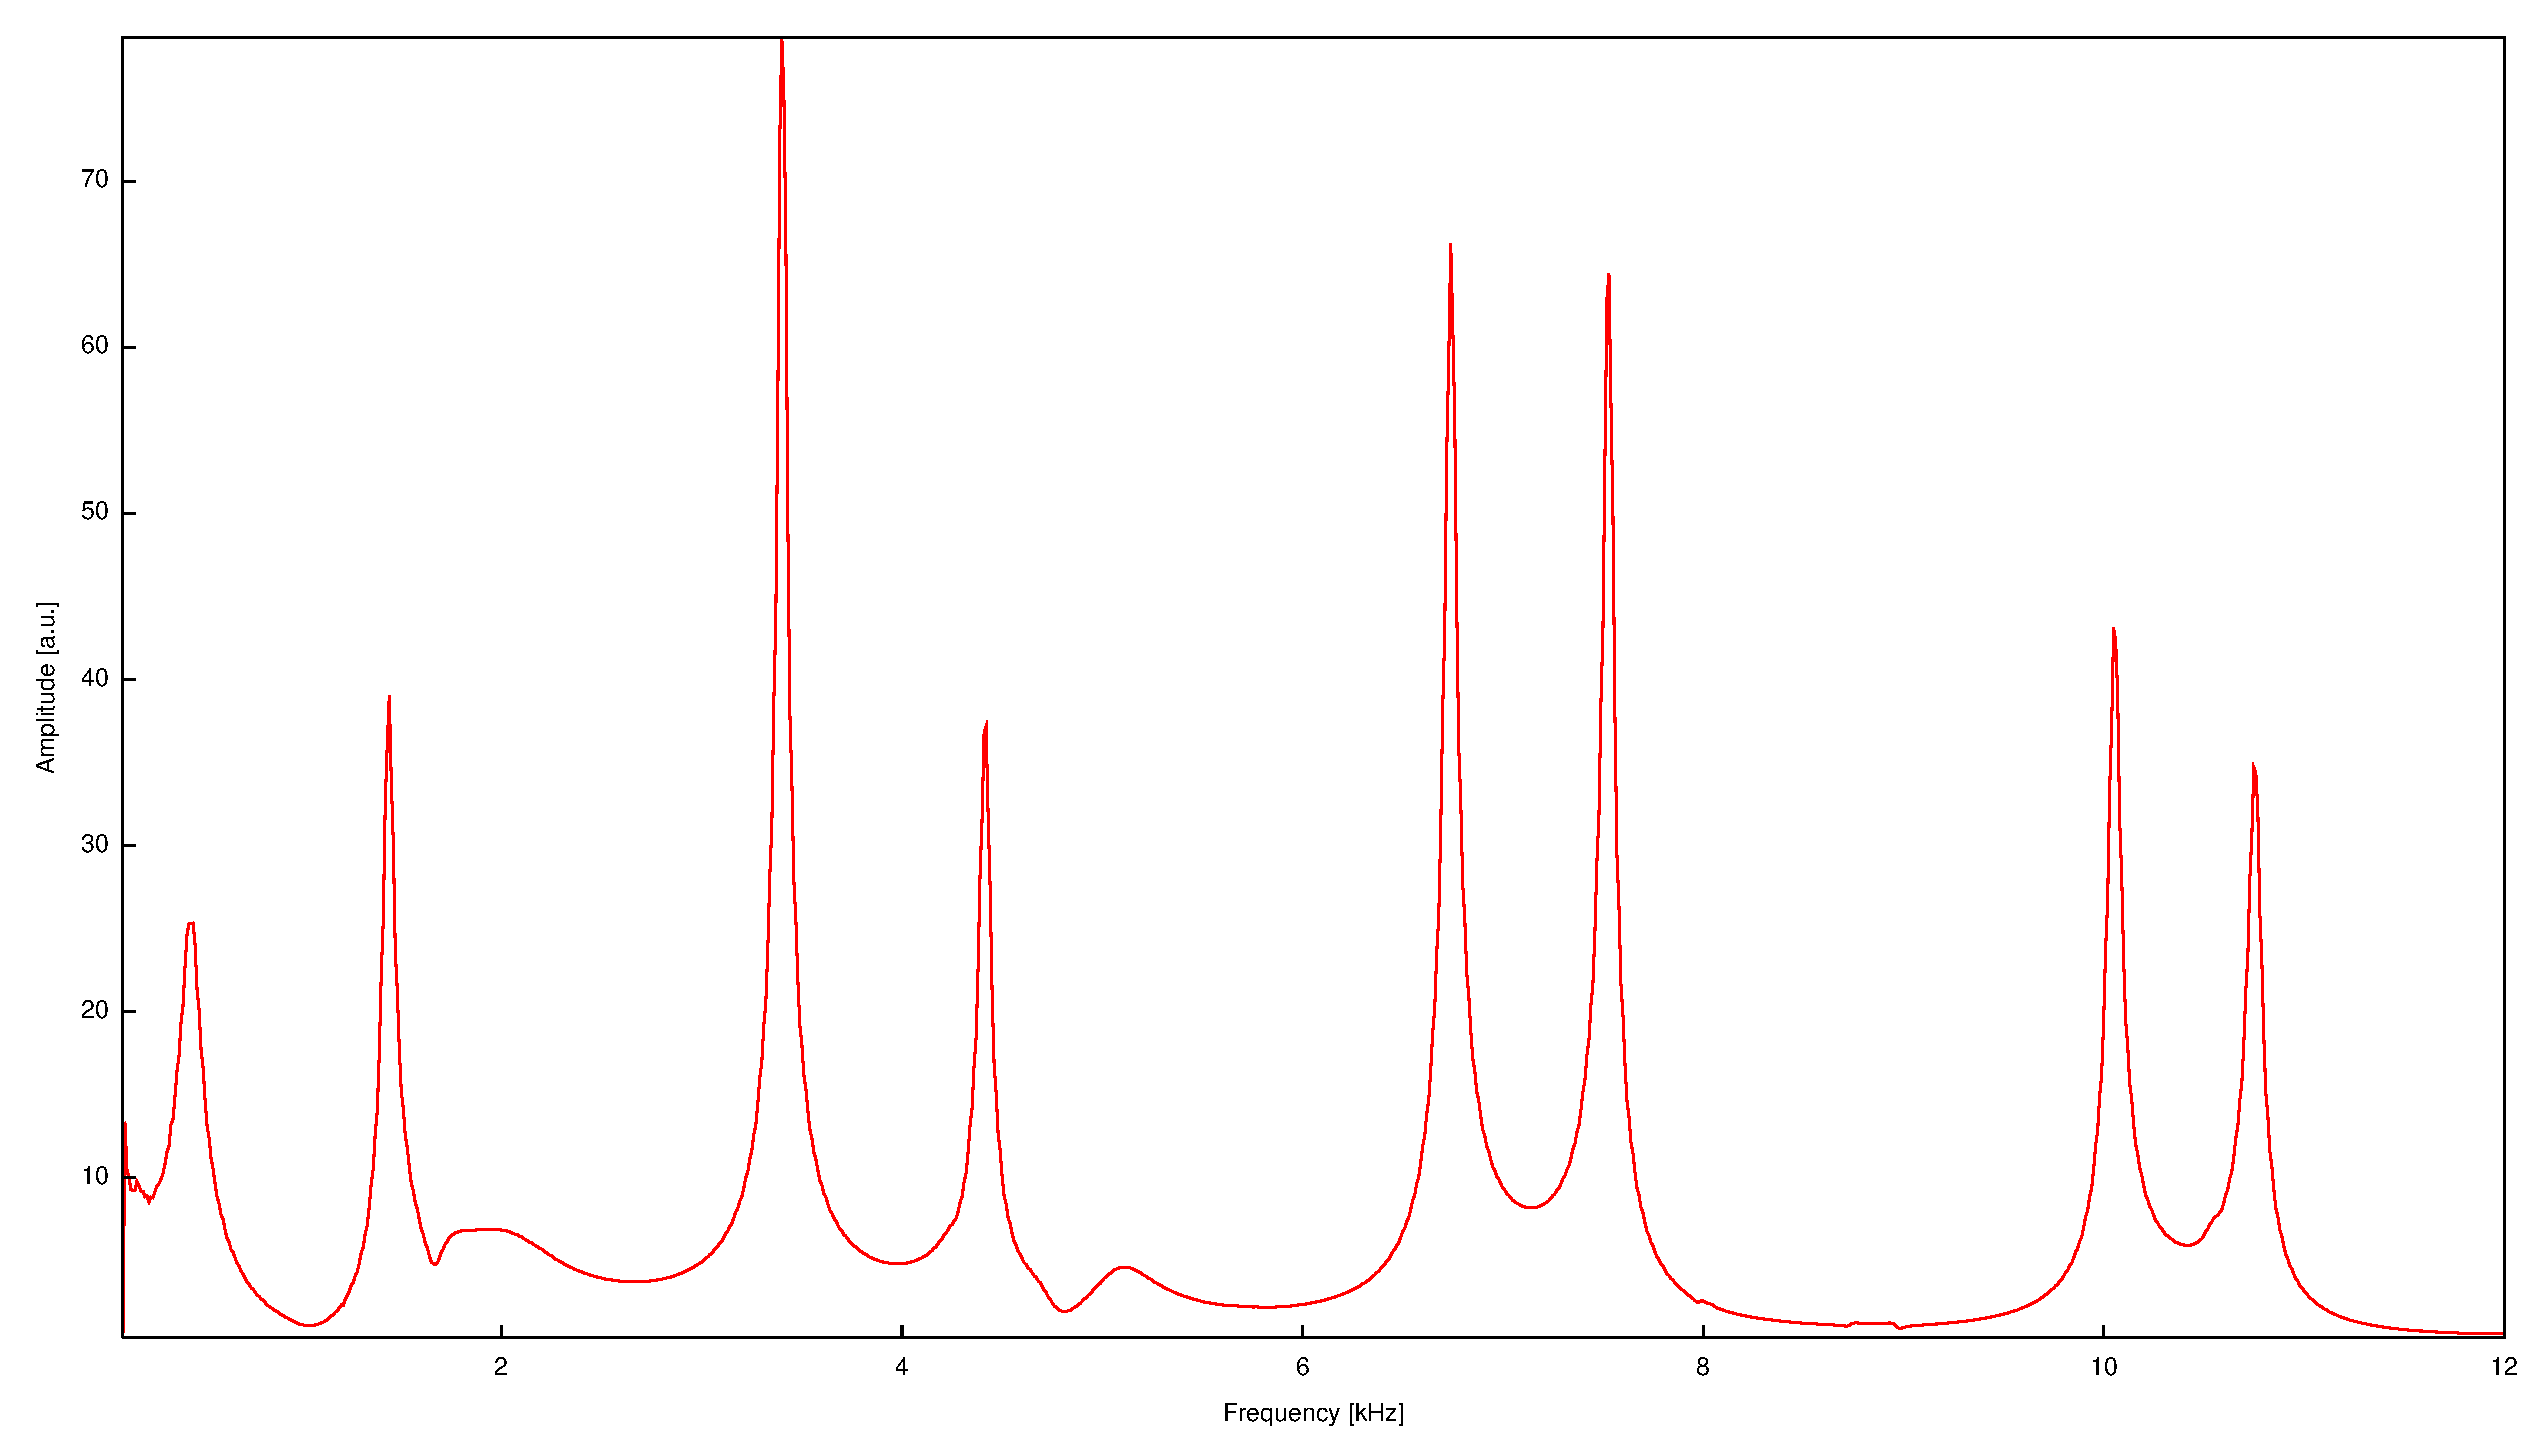
\includegraphics[width=\linewidth-60pt,height=\textheight-60pt,keepaspectratio]{FP-V23data/4.8_100mm_16mm.eps}
\caption{Spektrum von einer Einheitszelle bestehend aus zwei über $\SI{16}{\milli\meter}$-Iriden gekoppelten $\SI{50}{\milli\meter}$-Röhren.}
\label{fig:50_16_50}
\end{figure}

\newpage
\noindent In Abbildung \ref{fig:12_50_13_16} ist das Spektrum einer Folge von zwölf $\SI{50}{\milli\meter}$-Röhren, die abwechselnd über $\SI{13}{\milli\meter}$- und über $\SI{16}{\milli\meter}$-Iriden gekoppelt sind. Der Vergleich mit Abbildung \ref{fig:12_50_16} zeigt, dass sich bei alternierender Kopplung innerhalb der Bänder eine Substruktur bildet, die Anzahl der Peaks jedoch konstant bleibt. In den Abbildungen \ref{fig:4_10} und \ref{fig:4_10(4_4)} sind die Bandstrukturen im reduzierten Zonenschema zu sehen. 

\begin{figure}
\centering
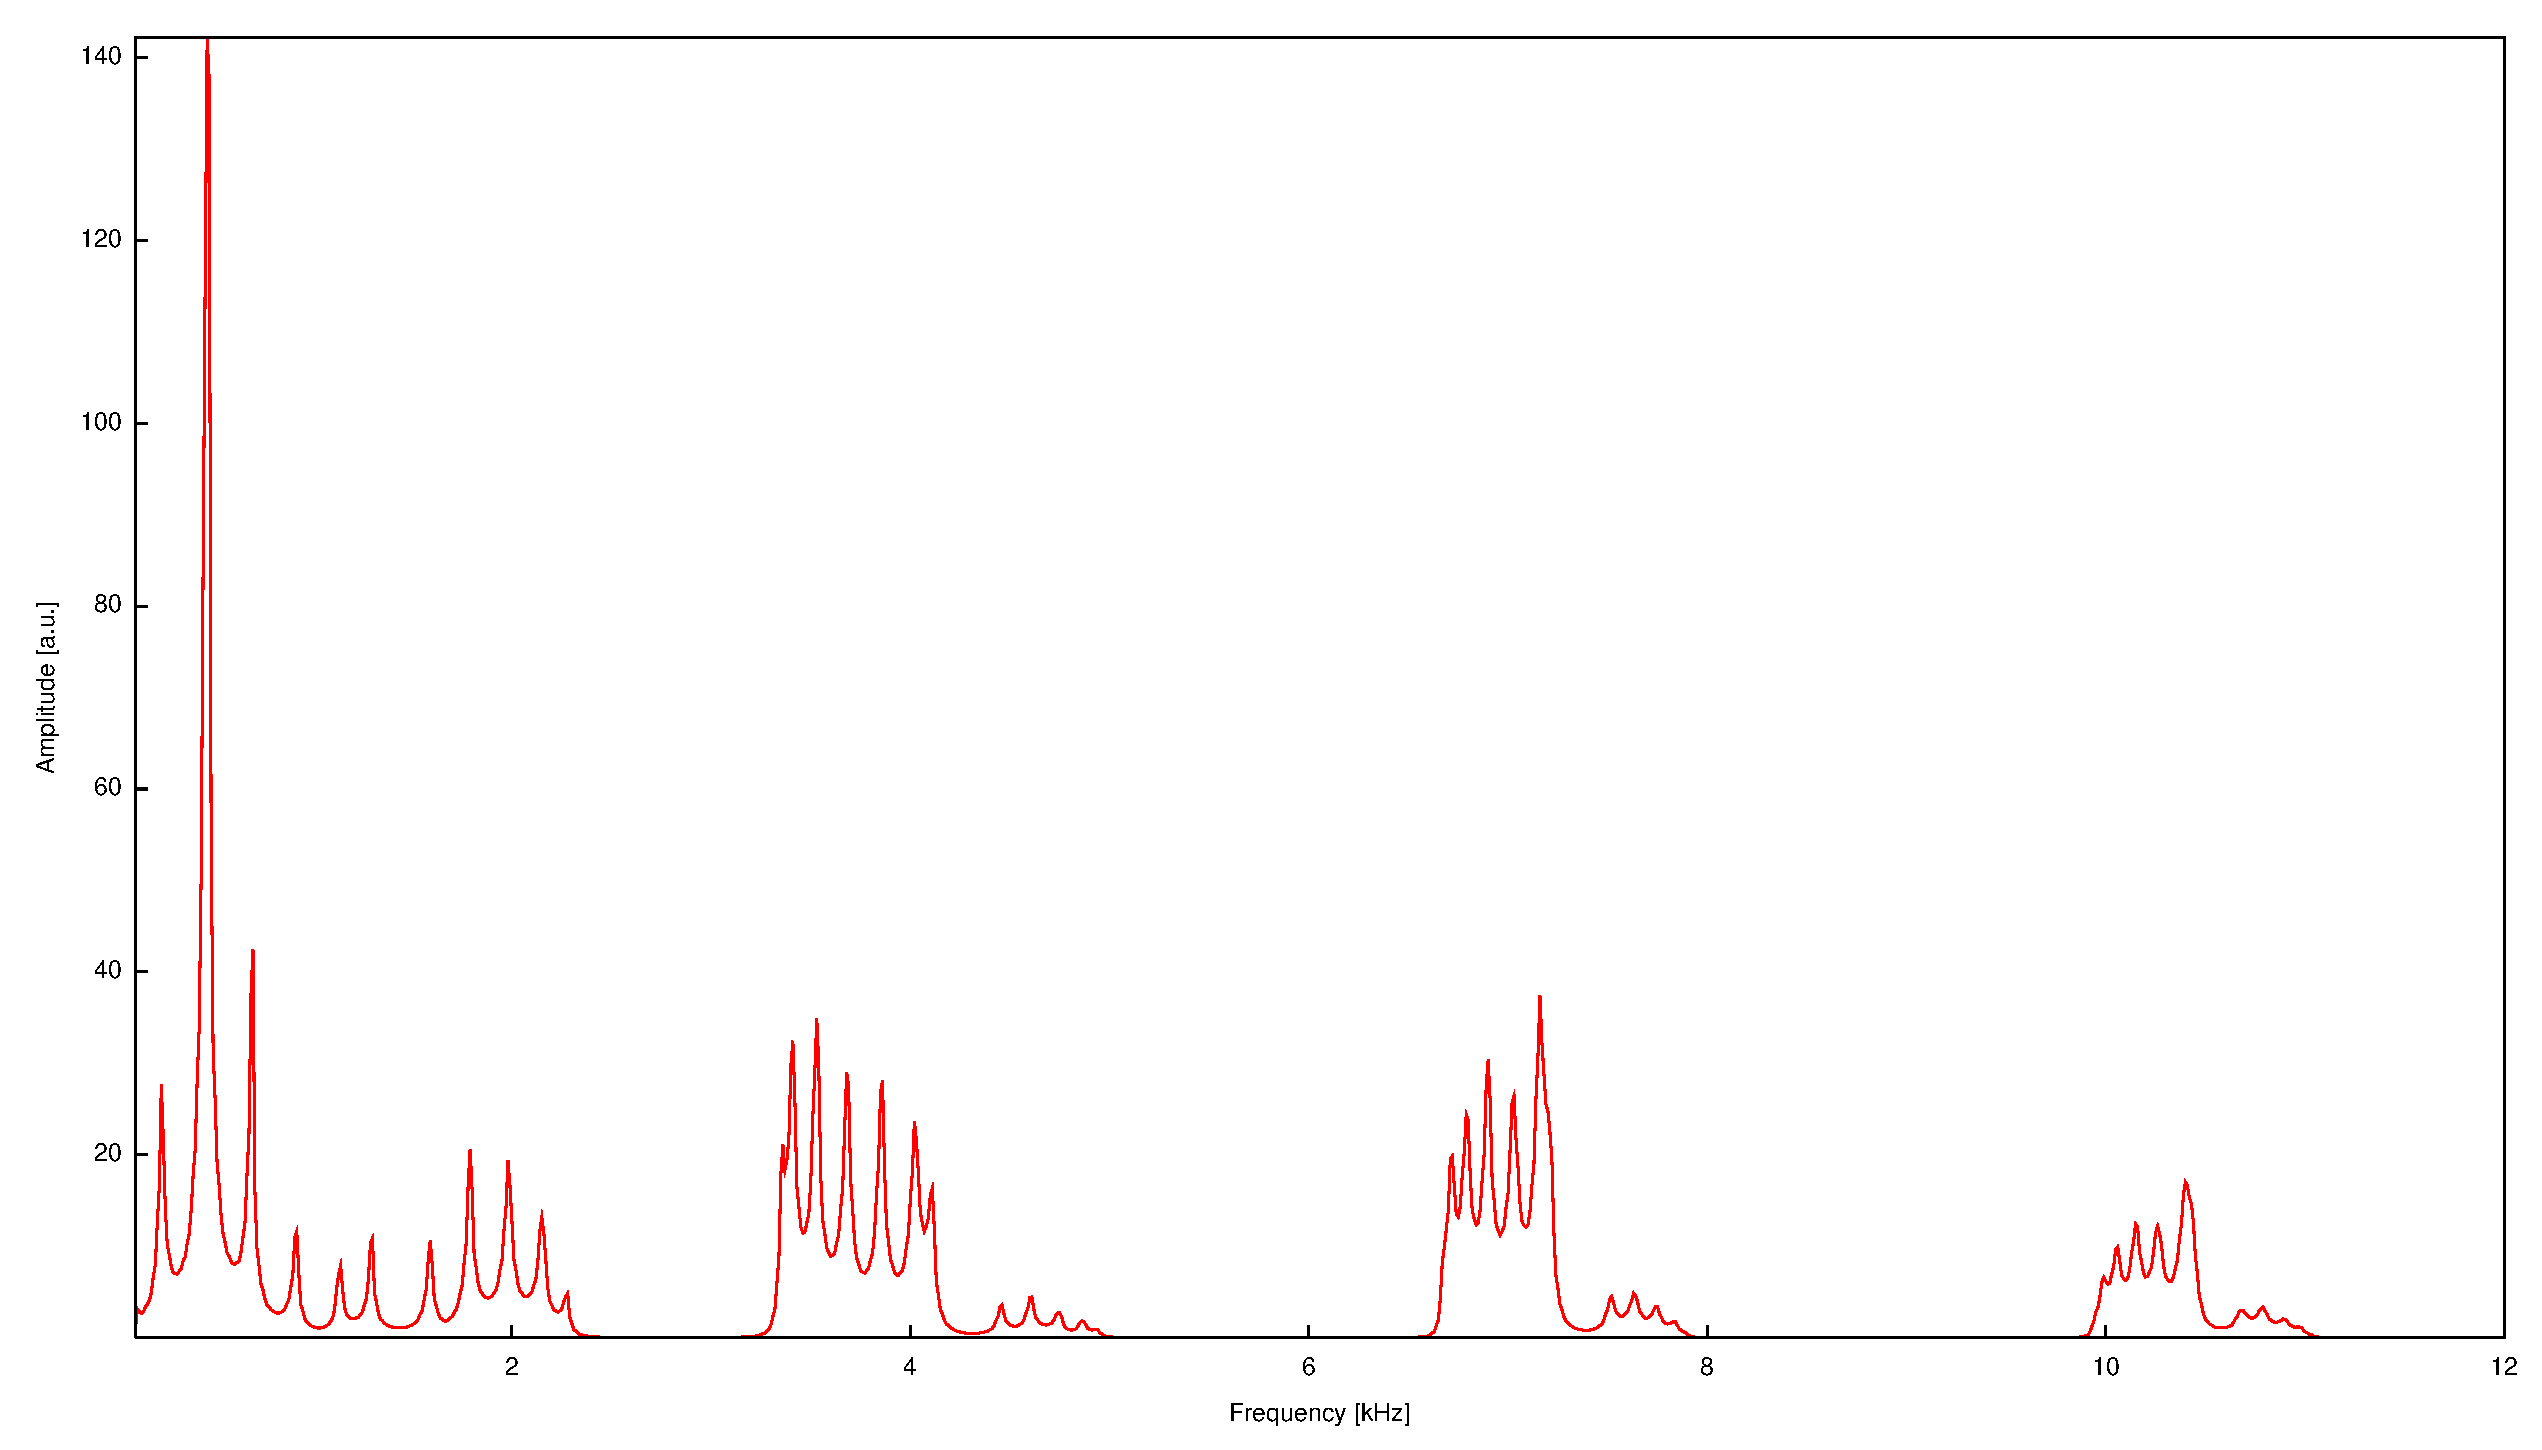
\includegraphics[width=\linewidth-60pt,height=\textheight-60pt,keepaspectratio]{FP-V23data/4.10_600mm_13_16mm.eps}
\caption{Spektrum von zwölf abwechselnd über $13$- und $\SI{16}{\milli\meter}$-Iriden gekoppelten $\SI{50}{\milli\meter}$-Röhren.}
\label{fig:12_50_13_16}
\end{figure}

\begin{figure}
\centering
\includegraphics[width=\linewidth-60pt,height=\textheight-60pt,keepaspectratio]{build/4.10_reduced.pdf}
\caption{Bandstruktur von zwölf abwechselnd über $13$- und $\SI{16}{\milli\meter}$-Iriden gekoppelten $\SI{50}{\milli\meter}$-Röhren.}
\label{fig:4_10}
\end{figure}

\begin{figure}
\centering
\includegraphics[width=\linewidth-60pt,height=\textheight-60pt,keepaspectratio]{build/4.10(4.4_600mm_16mm)_reduced.pdf}
\caption{Bandstruktur von zwölf über $\SI{16}{\milli\meter}$-Iriden gekoppelten $\SI{50}{\milli\meter}$-Röhren.}
\label{fig:4_10(4_4)}
\end{figure}

\newpage
\noindent In Abbildung \ref{fig:4.11} ist das Spektrum einer Folge von fünf Zellen bestehend aus einer $\SI{50}{\milli\meter}$-Röhre mit einer $\SI{16}{\milli\meter}$-Iris und einer $\SI{75}{\milli\meter}$-Röhre mit einer $\SI{16}{\milli\meter}$-Iris. In den Abbildungen \ref{fig:4_11_ext} und \ref{fig:4_11_red} sind die Bandstrukturen im erweiterten, wie im reduzierten Zonenschema zu sehen. Um das reduzierte Schema etwas anschaulicher zu machen, sind die Werte in einem Band mit einer Linie verbunden.\\
Es ist zu erkennen, dass sich jeweils zwei Bänder mit fünf Peaks ohne Bandlücke, gefolgt von drei Bändern mit fünf Peaks mit Bandlücke Bilden. Das Verhältnis von $\frac{2}{3}$ entspricht dem aus den atomaren Zellen aus den Abbildungen \ref{fig:50mm} und \ref{fig:75mm}.

\begin{figure}
\centering
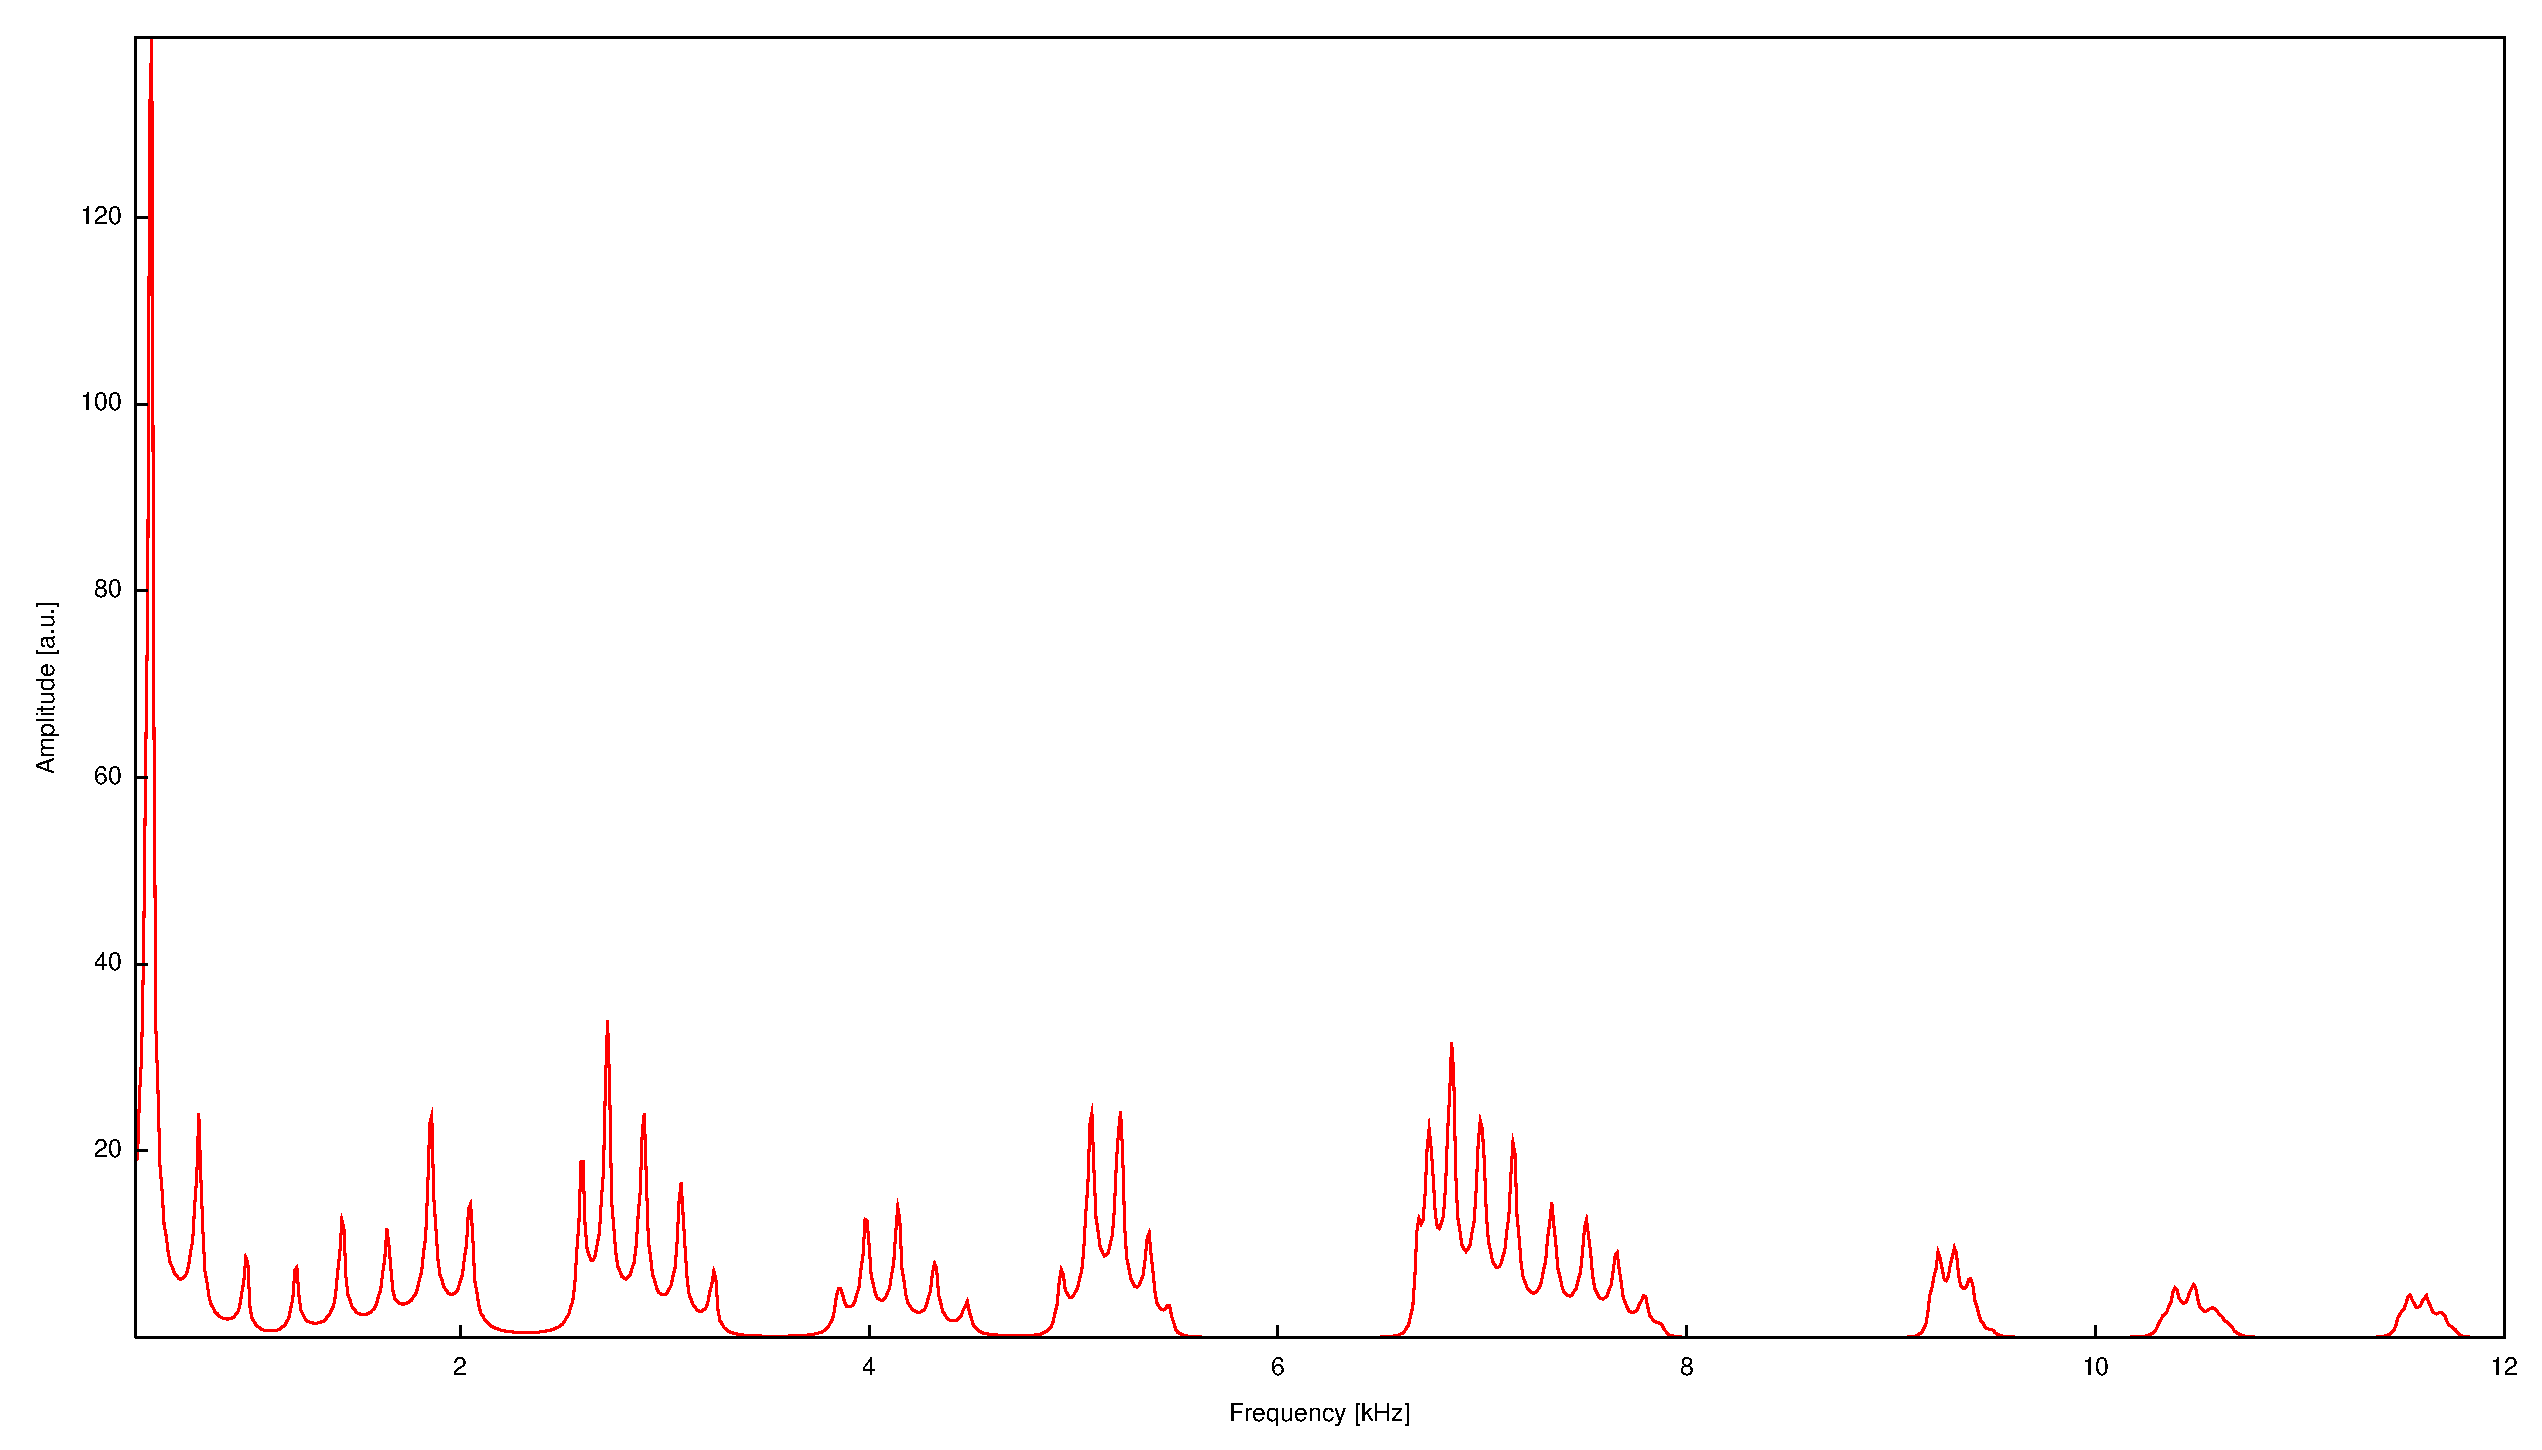
\includegraphics[width=\linewidth-60pt,height=\textheight-60pt,keepaspectratio]{FP-V23data/4.11_625mm_50_16_75mm.eps}
\caption{Spektrum von fünf Zellen bestehend aus einer $\SI{50}{\milli\meter}$-Röhre und einer $\SI{75}{\milli\meter}$-Röhre jeweils gekoppelt mit einer $\SI{16}{\milli\meter}$-Iris.}
\label{fig:4.11}
\end{figure}

\begin{figure}
\centering
\includegraphics[width=\linewidth-60pt,height=\textheight-60pt,keepaspectratio]{build/4.11_extended.pdf}
\caption{Bandstruktur von fünf Zellen bestehend aus einer $\SI{50}{\milli\meter}$-Röhre und einer $\SI{75}{\milli\meter}$-Röhre jeweils gekoppelt mit einer $\SI{16}{\milli\meter}$-Iris im erweiterten Schema.}
\label{fig:4_11_ext}
\end{figure}

\begin{figure}
\centering
\includegraphics[width=\linewidth-60pt,height=\textheight-60pt,keepaspectratio]{build/4.11_reduced.pdf}
\caption{Bandstruktur von fünf Zellen bestehend aus einer $\SI{50}{\milli\meter}$-Röhre und einer $\SI{75}{\milli\meter}$-Röhre jeweils gekoppelt mit einer $\SI{16}{\milli\meter}$-Iris im reduzierten Schema.}
\label{fig:4_11_red}
\end{figure}

\newpage
\noindent Im folgenden wird in einer Röhre bestehend aus $\SI{50}{\milli\meter}$-Röhren mit $\SI{16}{\milli\meter}$-Iriden eine Fehlstelle in Form einer $\SI{75}{\milli\meter}$-Röhre eingebaut.
In Abbildung \ref{fig:4.12_3} ist das Spektrum abgebildet, wenn das dritte Segment ausgetauscht wird.
Im Vergleich zum Aufbau ohne Defekt in Abbildung \ref{fig:12_50_16} ist zu erkennen, dass das zweite Band nur noch elf Peaks besitzt und sich ein neuer Defekt-Peak in der ersten Bandlücke bildet. Dieser ist unabhängig von der Position, an der das Segment ausgetauscht wird, jedoch abhängig von der Länge dieses Segments. Die Lage der Peaks im zweiten Band ändert sich leicht je nachdem wo das Fehlsegment platziert wird.\\
In den Abbildungen \ref{fig:4_12_1} und \ref{fig:4_12_2} sind die Bandstrukturen im reduzierten Zonenschema zu sehen.

\begin{figure}
\centering
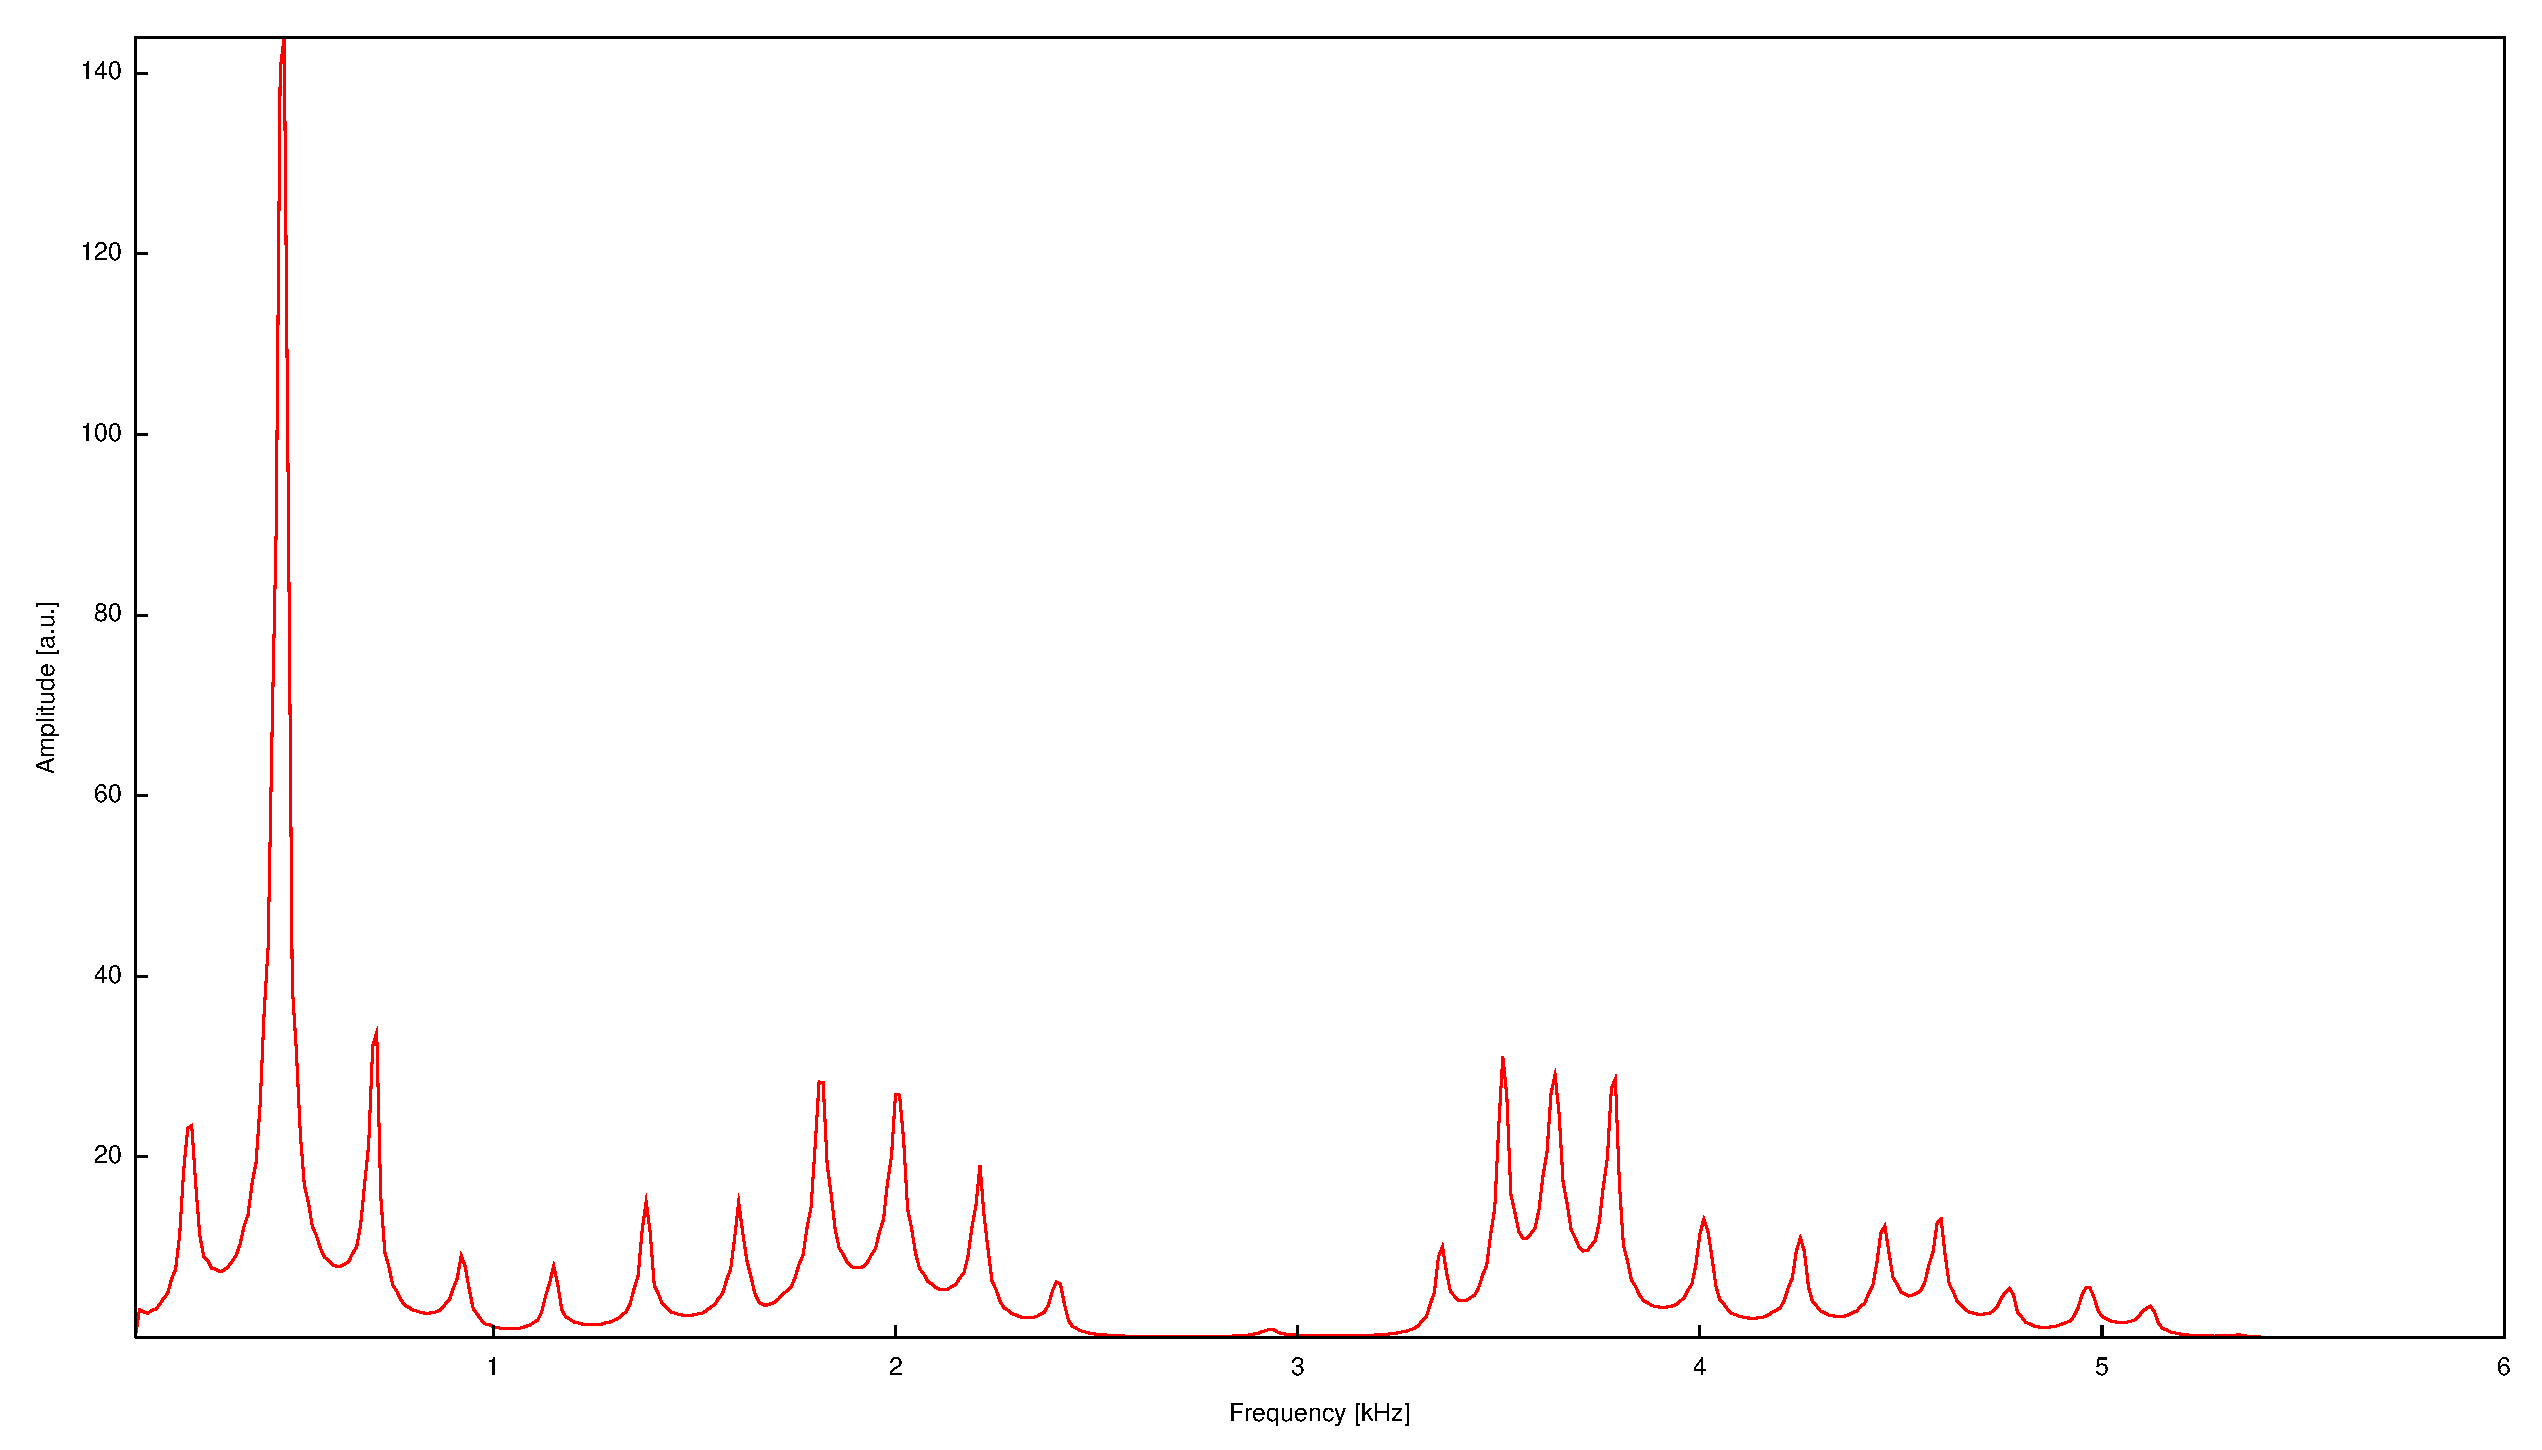
\includegraphics[width=\linewidth-60pt,height=\textheight-60pt,keepaspectratio]{FP-V23data/4.12_seg3_75mm.eps}
\caption{Spektrum einer Röhre bestehend aus $\SI{50}{\milli\meter}$-Röhren getrennt durch $\SI{16}{\milli\meter}$-Iriden mit einer $\SI{75}{\milli\meter}$ Fehlstelle im dritten Segment.}
\label{fig:4.12_3}
\end{figure}

\begin{figure}
\centering
\includegraphics[width=\linewidth-60pt,height=\textheight-60pt,keepaspectratio]{build/4.12_reduced.pdf}
\caption{Bandstruktur einer Röhre bestehend aus $\SI{50}{\milli\meter}$-Röhren getrennt durch $\SI{16}{\milli\meter}$-Iriden mit einer $\SI{75}{\milli\meter}$ Fehlstelle im dritten Segment.}
\label{fig:4_12_1}
\end{figure}

\begin{figure}
\centering
\includegraphics[width=\linewidth-60pt,height=\textheight-60pt,keepaspectratio]{build/4.12(4.4_600mm_16mm)_reduced.pdf}
\caption{Bandstruktur einer Röhre bestehend aus $\SI{50}{\milli\meter}$-Röhren getrennt durch $\SI{16}{\milli\meter}$-Iriden ohne Fehlstelle.}
\label{fig:4_12_2}
\end{figure}

%◘♦☻♥◘○☺♠◘
